\chapter{Investigation of Phthalate Esters in Proton Transfer Reaction Mass Spectrometry via Direct Headspace Sampling}\label{chapter:PH}
\markboth{Investigation of phthalates in PTR-MS}{}

%This chapter is a reformatted copy of my published article:

%\fullcite{phthalates}.

%\section*{Declaration of contribution}
%My contribution to the article of which the present chapter is composed of was
%performing the experiments, analysing the data and writing the manuscript. 

%\section{Abstract}

%\textbf{\textit{Keywords}}:



In this chapter, a study of the reactions of phthalic acid and ten phthalate esters with H$_3$O$^+$ in the reaction region of a PTR-MS instrument as a function of the drift voltage and the reduced electric field is presented.


\section{Introduction}

Phthalate esters, or simply phthalates, form a family of chemicals that are commonly used as plasticisers, mainly to soften polyvinyl chloride (PVC), and which are present in products of everyday use like clothing, food packaging, toys, building materials, pharmaceuticals and personal care products \cite{graham1973phthalate,cao2010phthalate,schettler2006human}.  
%
%
Plasticised products have become ubiquitous in  homes, schools and workplaces, and the exposure to phthalates has been proved to be higher than the tolerable daily intake (\acrshort{TDI}), being up to twenty times higher than this limit for children 
\cite{heudorf2007phthalates}.
%
%Phthalates from household waste can contaminate the environment as well and they have been found in environmental matrices (e.g. air and ground) \cite{bauer1997estimation}.








%\textbf{Exposure sources}
Phthalates are some of the pollutants that humans are the most exposed to.
%
The main routes of exposure to phthalates are through ingestion, inhalation and dermal absorption.
%
An extensive study of the  sources of exposure  for Europeans is that published by  \citeauthor{wormuth2006sources} \cite{wormuth2006sources}.
%
Ingestion of phthalates occurs mainly through food contamination in adults and through toys mouthing in children \cite{fan2012determination,earls2003gas}. 
%
%A LC–MS/MS study from 
 \citeauthor{xu2014determination} reported the presence of 23 phthalate esters in food samples (e.g. dairy, meat, oil and canned products) 
\cite{xu2014determination}.
%
Inhalation of phthalates  can occur in closed spaces where plasticised products are present and these contaminants  have migrated to the dust and the air.
%
\citeauthor{geiss2009investigation} found  variable concentrations between summer and winter of phthalates, particularly diethyl phthalate (DEP), dibutyl phthalate (DBP) and bis(2-ethylhexyl) phthalate (DEHP), inside used car cabins \cite{geiss2009investigation}.
%
These pollutants come predominantly from the car plastic parts and they can be present inside buildings as well, as PVC is a material often used in construction, for instance in vinyl flooring  \cite{gong2018letter}.
%
%For instance, the use of vinyl flooring also presents a phthalate inhalation hazard in buildings and closed environments \cite{gong2018letter}.
%
Regarding dermal absorption, the extended use of personal care products, like make up and contact lenses, are the main source of contamination, but dermal absorption can also occur through the use of medical equipment like plastic tubing and vinyl gloves \cite{perez2011presence,duty2005personal,calafat2004exposure}.



Phthalates are  %some of the most abundant  
endocrine-disrupting chemicals  %present in air 
and studies relate them to development and male reproductive toxicity while others suggest that they are not harmful to the female reproductive system \cite{rudel2003phthalates,foster2000effects,benson2009hazard,matsumoto2008potential,kay2013reproductive}. 
%
Experiments of  DEHP exposure  in mice suggest that it cannot be ruled out as a human carcinogen \cite{rusyn2012mechanistic}.
%
In children, the presence of phthalate metabolites in urine has been linked to attention deficit and hyperactivity disorder as well as  asthma \cite{kim2009phthalates,bornehag2010phthalate}.
%
Phthalates traces have been found in human blood and faeces and even in breastfeeding human milk \cite{de2014review,zhu2006phthalate}.
%
\citeauthor{duty2005personal} linked the presence of phthalates monoesters in urine to the use of personal care products \cite{duty2005personal}.
%
An extensive discussion of the metabolism of phthalates is that published from \citeauthor{frederiksen2007metabolism}, %\cite{frederiksen2007metabolism}.
while  
\citeauthor{wittassek2008phthalates} showed that the metabolism of DEHP consists mainly on oxidised products in urine and mono(2-ethylhexyl) phthalate (MEHP) is the primary metabolite in blood 
\cite{frederiksen2007metabolism,wittassek2008phthalates}.
%


%
%Phthalates migration from food packaging to food (solid phase extraction and UHPLC-MS/MS)  \cite{fan2012determination} and from toys \cite{earls2003gas}.

Because of the health risks they present, the use of phthalates has recently started to be controlled by the enforcing authorities in several countries. The EU has restricted since 2005 the use of phthalates as plasticisers in toys for kids, banning toys and childcare articles carrying more than  0.1\% mass of DBP, %dibutyl phthalate, 
benzyl butyl phthalate (BBP)  and DEHP, which are classified as reprotoxic  
\cite{Parliament2005}. 
A similar ban is imposed to diisononyl phthalate, diisodecyl phthalate and dioctyl phthalate, although scientific information is either lacking or conflictual.
US and China  implemented comparable regulations in 2008  and 2016 \cite{USban,chinaGB6675}.



    %%%Whether phthalates are harmful or not is still a matter of discussion, although the authorities have been implementing restrictions and bans like the ones mentioned earlier.
%
    %%%The main agreement so far within the scientific community with respect to phthalates is that further investigation is needed \cite{hauser2005phthalates}.
%
Health and environmental hazards arising from phthalates exposure and contamination has led to the application of several analytical techniques to the detection and quantification  of these substances.
%
Some of the applied techniques are
LC-MS/MS, %\cite{xu2014determination,net2015reliable}
GC-MS,  %\cite{GC-PICI-phthalates,net2015reliable}
EI-MS, %\cite{lacko2018dissociation}
IMS, IMS-MS, %\cite{michalczuk2019isomer}
ESI-HCD-MS %\cite{mzcloudd}
and
UHPLC-MS/MS %fan2012determination
 \cite{xu2014determination,net2015reliable,GC-PICI-phthalates,lacko2018dissociation,mzcloudd,michalczuk2019isomer,fan2012determination}.
%
%Phthalates in GC-PICI-SRM-MS have been detected at sub nanogram levels \cite{GC-PICI-phthalates}.
%
%Phthalates in IMS \cite{michalczuk2019isomer}.
%
%Phthalates in low-energy EI \cite{lacko2018dissociation}.
%
%Quantification of phthalates in environmental matrices (air, ground, etc) at ultra-trace levels  \cite{net2015reliable}
%
There are, however, no extensive studies of phthalates in PTR-MS as of today.
%
Also, the main agreement so far within the scientific community with respect to phthalates is that further investigation is needed \cite{hauser2005phthalates}.
%
These two reasons are the main motivation for the study presented here. 


In this chapter a study of the reactions of 
phthalic acid (PAcid\footnote{Phthalic acid is called PAcid instead of PA to avoid confusion with the abbreviation for proton affinity.}),                              %done
dimethyl phthalate (DMP),                     %done
diethyl phthalate (DEP),                     %done
diallyl phthalate (DAP),                       %done
dipropyl phthalate (DPP),                      %done
dibutyl phthalate (DBP),                       %done
monoethylhexyl phthalate (MEHP, also known as mono(2-ethylhexyl) phthalate),               %done
diisobutyl phthalate (DiBP),                   %done
benzyl butyl phthalate (BBP),                  %done
dibenzyl phthalate (DBeP)                         %done
and
diethylhexyl phthalate (DEHP, also known as bis(2-ethylhexyl) phthalate)                 %done
with H$_3$O$^+$ in the reaction region of a PTR-MS instrument as a function of the drift voltage and the reduced electric field is presented.



%%%%%%%%%%%%%%%%%%%%%%%%%%%%%%%%%%%%%%%%%%%%%%%%%%%%%%%%%%%%%%%%%%%%%%%%%%%%%%%%%%%%%%%%%%%%%%%%%%%%%%
\section{Methodology}

\subsection{Chemicals}
Phthalates are colourless to pale-yellow, oily liquids. Phthalic acid is a white powder.
The samples used for this study  are
%
%
PAcid (Sigma Aldrich, 99.5\%),                              %done
DMP (Acros Organics, 99\%),                     %done
DEP (Sigma Aldrich, 99.5\%),                     %done
DAP (Sigma Aldrich, 97\%),                       %done
DPP (Sigma Aldrich, 98\%),                      %done
DBP (Sigma Aldrich, 99\%),                       %done
MEHP (Sigma Aldrich, 97\%),               %done
DiBP (Sigma Aldrich, 99\%),                   %done
BBP (Sigma Aldrich, 98\%),                  %done
DBeP (Alfa Aesar, 97\%)                         %done
and
DEHP (Sigma Aldrich, 96\%). %done
%
%
%
%
%The samples acquired for this study  are
%phthalic acid (PAcid\footnote{Phthalic acid is called PAcid instead of PA to avoid confusion with the abbreviation for proton affinity.}, Sigma Aldrich, 99.5\%),                              %done
%dimethyl phthalate (DMP, Acros Organics, 99\%),                     %done
%diethyl phthalate (DEP, Sigma Aldrich, 99.5\%),                     %done
%diallyl phthalate (DAP, Sigma Aldrich, 97\%),                       %done
%dipropyl phthalate (DPP, Sigma Aldrich, 98\%),                      %done
%dibutyl phthalate (DBP, Sigma Aldrich, 99\%),                       %done
%monoethylhexyl phthalate (MEHP, also known as mono(2-ethylhexyl) phthalate, Sigma Aldrich, 97\%),               %done
%diisobutyl phthalate (DiBP, Sigma Aldrich, 99\%),                   %done
%benzyl butyl phthalate (BBP, Sigma Aldrich, 98\%),                  %done
%dibenzyl phthalate (DBeP, Alfa Aesar, 97\%)                         %done
%and
%diethylhexyl phthalate (DEHP, also known as bis(2-ethylhexyl) phthalate, Sigma Aldrich, 96\%). %done
%
%
%
%
They were used without further purification.
%
The structure of these substances is provided in \autoref{tab:PH_structs}
%
The vapour pressure data at 25$^\circ$C was taken from the \citeauthor{USAEPA} database \cite{USAEPA}. The vapour pressure values for DAP, MEHP, DiBP and DBeP are the predicted ones while the ones for the rest of compounds were experimentally measured.

{\small

\begin{table}
\centering
\caption{Vapour pressure at 25$^\circ$C and structure of phthalic acid, dimethyl phthalate, diethyl phthalate, diallyl phthalate, dipropyl phthalate, dibutyl phthalate, monoethylhexyl phthalate, diisobutyl phthalate, benzyl butyl phthalate, dibenzyl phthalate and diethylhexyl phthalate.}
\begin{tabular}{lcc}
\textbf{Compound} &  \textbf{VP (mbar)} &  \textbf{Structure} \\ 
\toprule
PAcid &   8.48$\times$10$^{-7}$ &  \begin{minipage}[c]{0.35\linewidth}\centering
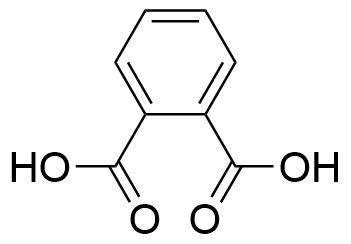
\includegraphics[height=0.07\textheight]{pics/PH/PAcid_struct2.png}\end{minipage}\\ \midrule
DMP &    4.11$\times$10$^{-3}$ &  \begin{minipage}[c]{0.35\linewidth}\centering
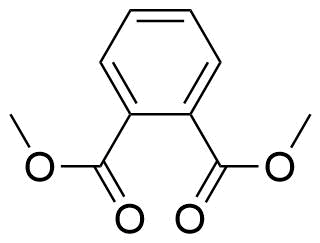
\includegraphics[height=0.07\textheight]{pics/PH/DMP_struct2.png}\end{minipage}\\ \midrule
DEP &   2.80$\times$10$^{-3}$ &  \begin{minipage}[c]{0.35\linewidth}\centering
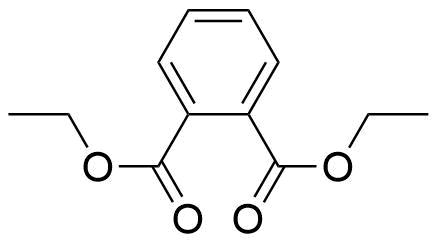
\includegraphics[height=0.07\textheight]{pics/PH/DEP_struct2.png}\end{minipage}\\ \midrule
DAP &   2.68$\times$10$^{-4}$  &  \begin{minipage}[c]{0.35\linewidth}\centering
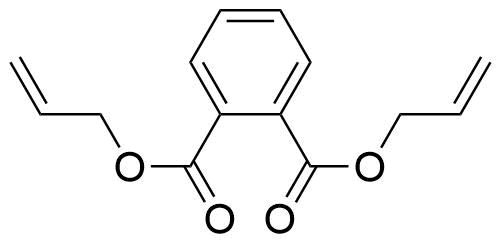
\includegraphics[height=0.07\textheight]{pics/PH/DAP_struct2.png}\end{minipage}\\ \midrule
DPP &   1.76$\times$10$^{-4}$ &  \begin{minipage}[c]{0.35\linewidth}\centering
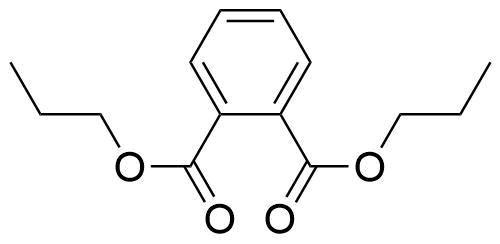
\includegraphics[height=0.07\textheight]{pics/PH/DPP_struct2.png}\end{minipage}\\ \midrule
DBP &   2.68$\times$10$^{-5}$ &  \begin{minipage}[c]{0.35\linewidth}\centering
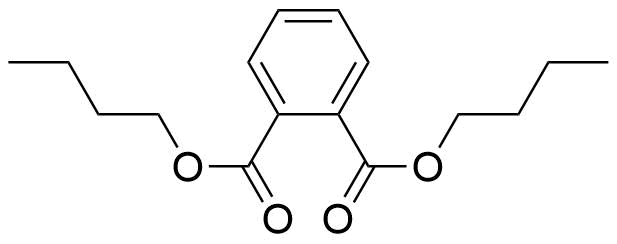
\includegraphics[height=0.07\textheight]{pics/PH/DBP_struct2.png}\end{minipage}\\ \midrule
MEHP &  1.08$\times$10$^{-6}$  &  \begin{minipage}[c]{0.35\linewidth}\centering
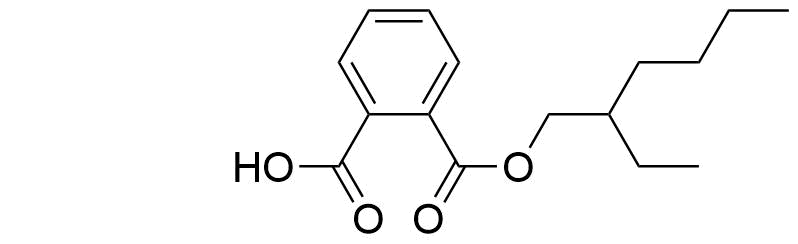
\includegraphics[height=0.07\textheight]{pics/PH/MEHP_struct3.png}\end{minipage}\\ \midrule
DiBP &  5.41$\times$10$^{-4}$   &  \begin{minipage}[c]{0.35\linewidth}\centering
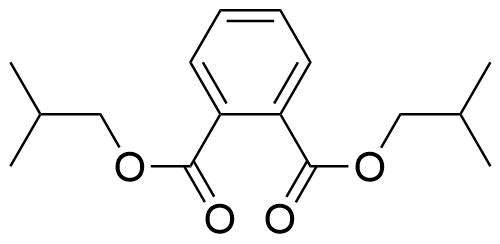
\includegraphics[height=0.07\textheight]{pics/PH/DiBP_struct2.png}\end{minipage}\\ \midrule
BBP &   1.10$\times$10$^{-5}$  &  \begin{minipage}[c]{0.35\linewidth}\centering
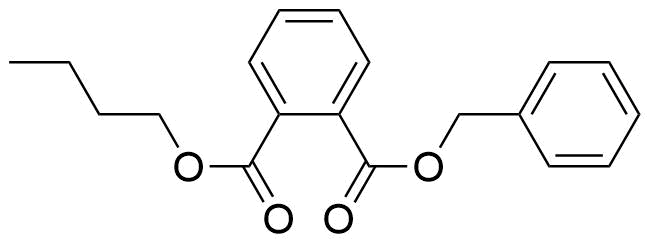
\includegraphics[height=0.07\textheight]{pics/PH/BBP_struct2.png}\end{minipage}\\ \midrule
DBeP &  1.59$\times$10$^{-6}$   &  \begin{minipage}[c]{0.35\linewidth}\centering
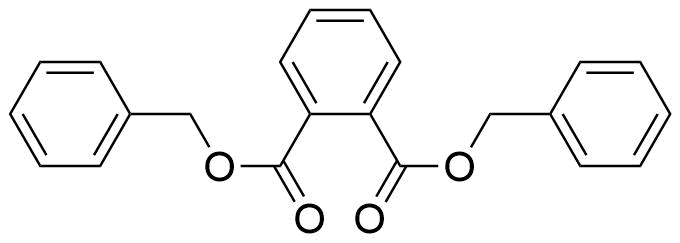
\includegraphics[height=0.07\textheight]{pics/PH/DBeP_struct2.png}\end{minipage}\\ \midrule
DEHP &  1.89$\times$10$^{-7}$   &  \begin{minipage}[c]{0.35\linewidth}\centering
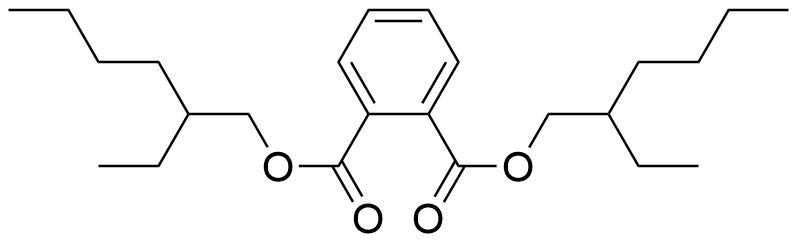
\includegraphics[height=0.07\textheight]{pics/PH/DEHP_struct2.png}\end{minipage}\\ 
\bottomrule
\end{tabular}
\label{tab:PH_structs}
\end{table}

}%small font closing



\subsection{Experimental details}

The analytical tool used for this study was the KORE Technology Ltd PTR-ToF-MS instrument described in \autoref{chapter:ptr}.
%
The hollow cathode was set at a pressure of 1.15 mbar while the drift tube pressure was at 1.10 mbar.
%
This was found to give the driest conditions in the reactor.
%
As \autoref{fig:PH_RI} reveals, the branching  percentage of H$_3$O$^+$ is   97\% or more for any reduced electric field while the contribution of  (H$_2$O)H$_3$O$^+$ to the total reagent ion signal is 3\% or less.
%
The inlet line and the oven were maintained both at 100\textsuperscript{$\circ$}C.
%
The experimental data for each phthalate was obtained by averaging two 10-second measurements for each \textit{E/N} value, which was manipulated keeping constant both  the drift tube pressure and  temperature and only changing the drift voltage  from approximately 160 V to 410 V to give a reduced electric field range of roughly 80 to 205 Td.



        \begin{figure}[htb]%[htbp]
        \centering
        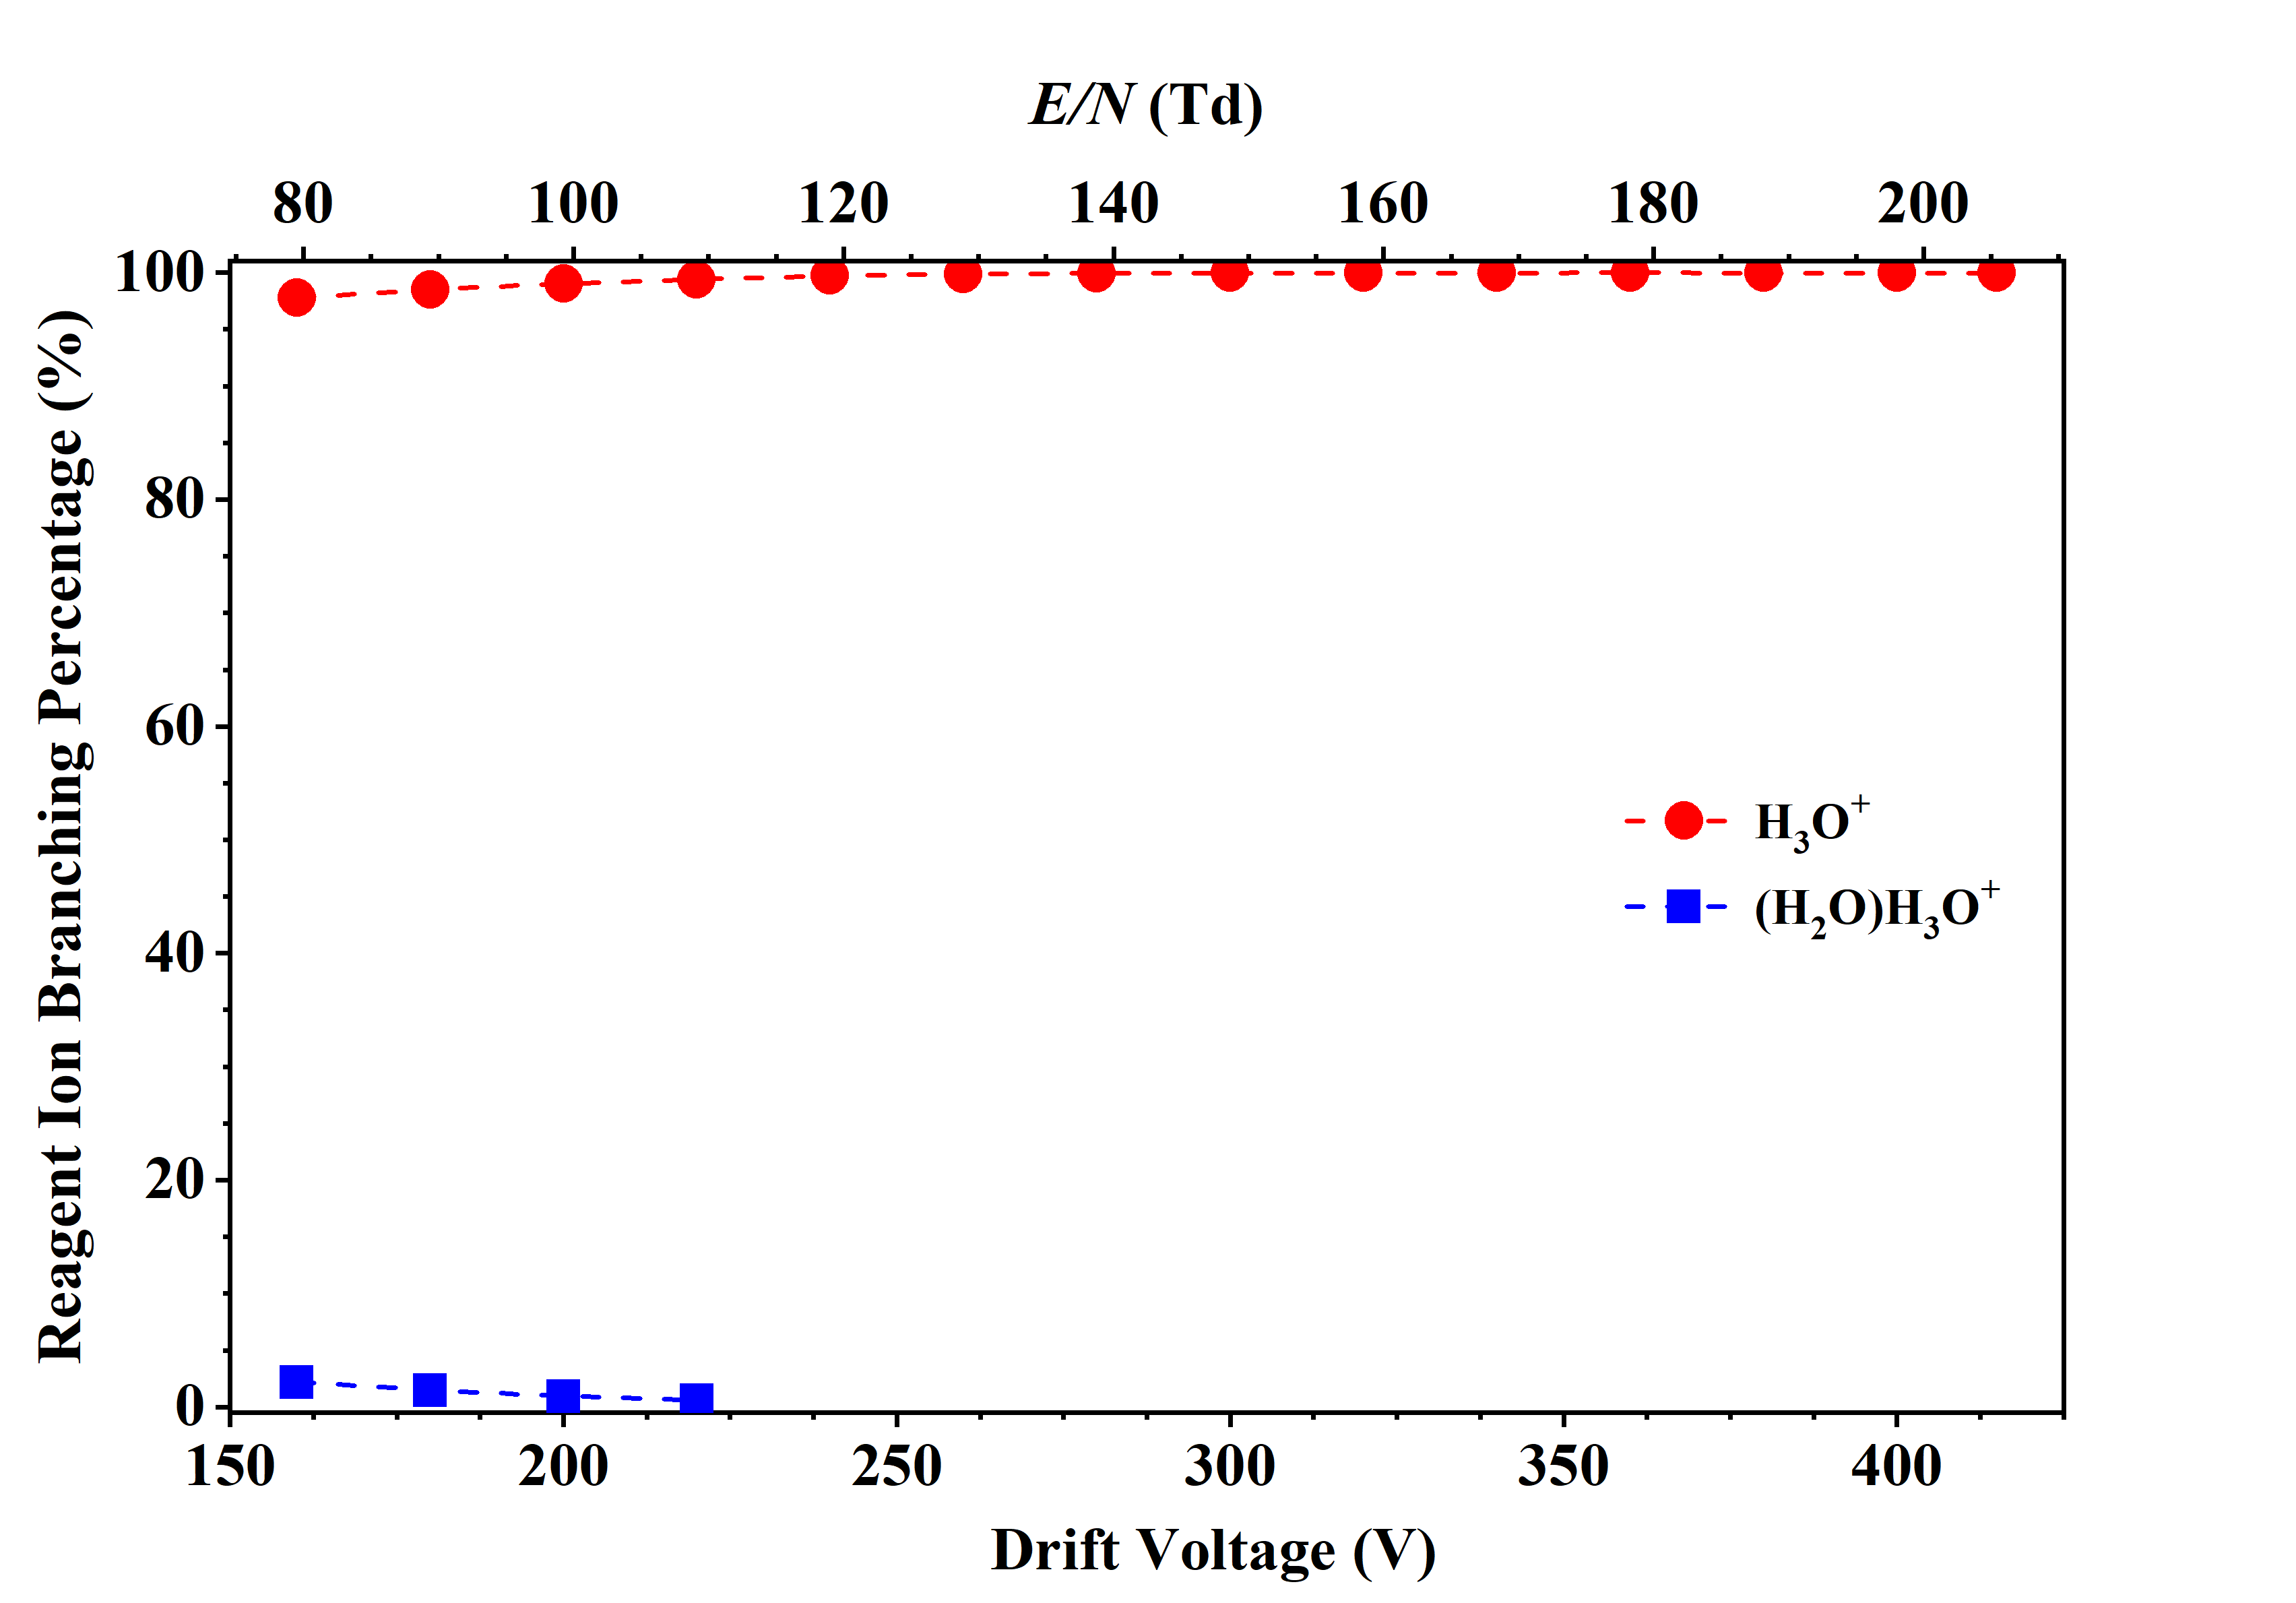
\includegraphics[height=0.4\textheight]{pics/PH/RI-BR.png}
        \caption{Reagent ion distribution plot as a function of the drift voltage and the \textit{E/N}.}
        \label{fig:PH_RI}
        \end{figure}



%Sampling method was headspace analysis.
%________________________________________________________ARTICLE__________________________

The phthalates were analysed via headspace sampling. 
%
40 mL amber vials containing 1-5 mL of  phthalate samples were connected to the inlet pipe of the PTR-ToF-MS to sample the headspace of said vial using oxygen-free nitrogen (99.998\% purity, BOC Gases, Manchester, UK) as carrier gas.
%
The vial was heated for the substances with the lowest vapour pressure  %(using some heating wire and a bench power supply, Range for the heating of the vial: 1 A in heating wire is equal to 100\textsuperscript{$\circ$}C. Obviously, 0.5 A is 50\textsuperscript{$\circ$}C.) 
to reach an ion intensity of at least 1000 %-3000 
 cps in the main product ions  at an \textit{E/N} of 120 Td.
%



The data acquisition was started only after approximately 30 minutes of preparing the experimental set up to avoid contamination.
%
Even though the purity of the samples was of at least 95\%, some volatile impurities were observed when the vials were first connected to the inlet line.
%
The product ions arising from these substances were found to steadily decrease and disappear in approximately 10-15 minutes while the phthalate product ions showed a stable behaviour throughout.
%
Also, the presence of impurities with similar volatility than the phthalates cannot be discarded either. 
%
For this reason, only the  ions that are identified as phthalate products and that represent more than 3\% of the total product ion signal are included here.
%
Due to the lack of comparable studies in the literature, the mzCloud mass spectral database was proved very useful to aid in the ion identification process \cite{mzcloudd}.
%
 This database contains, among others, electrospray ionisation (\acrshort{esi}) higher-energy collisional dissociation (\acrshort{hcd}) MS$^n$ results of tens of thousands of chemicals, which, at the lower-energy end,  are qualitatively comparable to PTR-MS and therefore mzCloud references\footnote{Note that the url in these references must be opened using Internet Explorer or the mzCloud desktop app \cite{mzcloudd}.}  are given for many compounds in this chapter to support and/or argue the findings of this study.
 
 %the mass analyser is usually an orbitrap, which allows to acquire MS$^n$ data  to study the fragmentation of the parent molecule or selected fragments with a very high mass resolution.% reducing the false positives and with a very high mass resolution (i.e ).


%N$_2$ flow of 0.3 L/min or 300 sccm into vial. 





\section{Results and discussion}

The reaction of the phthalate esters with (H$_2$O)$_n$H$_3$O$^+$ for n>0 is negligible in the present PTR-MS results because of the low abundance of these reagent ions (see \autoref{fig:PH_RI}) and hence only reactions with H$_3$O$^+$ are considered here (except for phthalic acid).
%
Furthermore, only the proton affinity of DMP (ca. 940 kJ mol$^{-1}$) %(936 - 942 kJ mol$^{-1}$)
is known, with \citeauthor{doi:10.1063/1.556018}  only having reported the proton affinity for two DMP isomers: dimethyl isophthalate (843.5 kJ mol$^{-1}$) and dimethyl terephthalate (843.2 kJ mol$^{-1}$), which are not included in this study \cite{michalczuk2019isomer,doi:10.1063/1.556018}.
%
The PA is hence unknown for the rest of the studied substances although they will  be higher than that of water because they undergo proton transfer with H$_3$O$^+$, and, by comparison  to the value for DMP from \citeauthor{michalczuk2019isomer}, it is likely that they will be also higher than that of the water dimer.
 
 \autoref{table:PID} shows a summary of the observed product ions and their associated percentage product ion distributions at \textit{E/N} values of 100, 140 and 180 Td resulting from the reactions of H$_3$O$^+$ with each of the studied phthalate samples. 
%
The most common fragmentation pathway observed in the present study is the loss of the two %phthalate
ester branches and an oxygen atom in the form of an alcohol molecule, as indicated in \autoref{fig:PH_fr}, to form protonated phthalic anhydride (i.e. \textit{m/z} 149).
%
This ion is not observed with all the phthalates (e.g. dimethyl and diallyl phthalate).%, but when this is a product ion its abundance increases with the reduced electric field, which indicates that the fragmentation is collision-induced.
%
Another common product ion is the one arising from the loss of a formate ester group.
%
A more complete diagram of the possible fragmentation pathways for the phthalates is  given by \citeauthor{yin2014mass} for electron impact ionisation \cite{yin2014mass}.

% If longtable does not split over pages, remove the afterpage
\afterpage{% for longtable to start in new page
% font needs to be smaller
{\small

\begin{longtable}[c]{lllccc}
\caption{Product ions identified and their associated percentage product ion distributions measured at reduced electric fields of 100, 140, and 180 Td resulting
from the reactions of H$_3$O$^+$ with several phthalate esters in order of increasing monoisotopic mass.} 
\label{table:PID}\\
\hline 
\textbf{Phthalate}& \textbf{Product ion \textit{m/z}} & \textbf{Product ion}  & \multicolumn{3}{c}{\textbf{PID (\%)}} \\ \cline{4-6} 
\textbf{Molecular formula} &\textbf{(Th)}&   \textbf{formula }& \multicolumn{3}{c}{\textbf{\textit{E/N} (Td)}} \\ \cline{4-6} 
\textbf{Monoisotopic mass (g/mol)  }      &                      &                     & \textbf{100 }     & \textbf{140}     & \textbf{180}  \\
\hline
\endfirsthead
\hline 
\textbf{Phthalate}& \textbf{Product ion \textit{m/z}} & \textbf{Product ion}  & \multicolumn{3}{c}{\textbf{PID (\%)}} \\ \cline{4-6} 
\textbf{Molecular formula} &\textbf{(Th)}&   \textbf{formula }& \multicolumn{3}{c}{\textbf{\textit{E/N} (Td)}} \\ \cline{4-6} 
\textbf{Monoisotopic mass (g/mol)  }      &                      &                     & \textbf{100 }     & \textbf{140}     & \textbf{180}  \\
\hline
\endhead
%
  (Continues on next page.)
\endfoot
%
\endlastfoot
PAcid   & 149.02  & C$_8$H$_5$O$_3^+$  & 98  & 100  & 100   \\
C$_8$H$_6$O$_4$  & 167.03  & (C$_8$H$_6$O$_4$)H$^+$  & 2  & 0  & 0  \\
166.03  & & & & &  \\
\hline
DMP       &    163.04    &  C$_9$H$_7$O$_3^+$   & 77 & 93 & 99   \\
C$_{10}$H$_{10}$O$_4$          &    195.07            & (C$_{10}$H$_{10}$O$_4$)H$^+$ & 23& 7& 1\\
194.06          & &  & & & \\
\hline
DEP       & 75.04                & C$_3$H$_7$O$_2^+$      & 7            & 1            & 0            \\
C$_{12}$H$_{14}$O$_4$          & 149.02               & C$_8$H$_5$O$_3^+$      & 1            & 7            & 76           \\
222.09          & 177.05               & C$_{10}$H$_9$O$_3^+$     & 36           & 57           & 21           \\
          & 223.10                & (C$_{12}$H$_{14}$O$_4$)H$^+$ & 56           & 35           & 3            \\
\hline
DAP                                                      & 39.02  & C$_3$H$_3^+$                        & 0  & 0  & 15 \\
C$_{14}$H$_{14}$O$_4$ & 41.04  & C$_3$H$_5^+$                        & 2  & 3  & 24 \\
246.09                                                   & 81.07  & C$_6$H$_9^+$                        & 4  & 10 & 19 \\
                                                         & 189.06 & C$_{11}$H$_9$O$_3^+$     & 10 & 27 & 29 \\
                                                         & 247.10  & (C$_{14}$H$_{14}$O$_4$)H$^+$ & 84 & 60 & 13\\
\hline
DPP       & 79.05                & C$_6$H$_7^+$                           & 1            & 1            & 5            \\
C$_{14}$H$_{18}$O$_4$          & 105.03               & C$_7$H$_5$O$^+$                          & 4            & 5            & 5            \\
250.12          & 123.04               & C$_7$H$_7$O$_2^+$      & 3            & 19           & 25           \\
          & 149.02               & C$_8$H$_5$O$_3^+$      & 3            & 21           & 54           \\
          & 165.09               & C$_{10}$H$_{13}$O$_2^+$    & 31           & 15           & 2            \\
          & 191.03               & C$_{11}$H$_{11}$O$_3^+$    & 15           & 6            & 2            \\
          & 251.13               & (C$_{14}$H$_{18}$O$_4$)H$^+$ & 43           & 33           & 7            \\
\hline
DBP                                                      & 79.05  & C$_6$H$_7^+$                        & 0  & 0  & 3  \\
C$_{16}$H$_{22}$O$_4$ & 105.03 & C$_7$H$_5$O$^+$                       & 4  & 5  & 5  \\
278.15                                                   & 123.04 & C$_7$H$_7$O$_2^+$      & 8  & 15 & 13 \\
                                                         & 149.02 & C$_8$H$_5$O$_3^+$      & 15 & 41 & 68 \\
                                                         & 179.10  & C$_{11}$H$_{15}$O$_2^+$    & 14 & 5  & 1  \\
                                                         & 205.09 & C$_{12}$H$_{13}$O$_3^+$    & 19 & 4  & 2  \\
                                                         & 279.16 & (C$_{16}$H$_{22}$O$_4$)H$^+$ & 40 & 30 & 8 \\
\hline
MEHP                                                     & 39.02  & C$_3$H$_3^+$                   & 0  & 1  & 15 \\
C$_{16}$H$_{22}$O$_4$ & 41.04  & C$_3$H$_5^+$                   & 0  & 5  & 12 \\
278.15                                                   & 43.05  & C$_3$H$_7^+$                   & 1  & 7  & 4  \\
                                                         & 57.07  & C$_4$H$_9^+$                   & 17 & 18 & 6  \\
                                                         & 69.07  & C$_5$H$_9^+$                   & 2  & 7  & 3  \\
                                                         & 71.09  & C$_5$H$_{11}^+$                  & 17 & 7  & 2  \\
                                                         & 111.12 & C$_8$H$_{15}^+$                  & 6  & 3  & 0  \\
                                                         & 113.13 & C$_8$H$_{17}^+$                  & 6  & 1  & 0  \\
                                                         & 129.13 & C$_8$H$_{17}$O$^+$                 & 10 & 5  & 2  \\
                                                         & 149.02 & C$_8$H$_5$O$_3^+$ & 41 & 46 & 56 \\
\hline
DiBP      & 57.07                & C$_4$H$_9^+$                           & 2            & 3            & 5            \\
C$_{16}$H$_{22}$O$_4$          & 149.02               & C$_8$H$_5$O$_3^+$      & 7            & 17           & 65           \\
278.15          & 205.09               & C$_{12}$H$_{13}$O$_3^+$    & 3            & 1            & 1            \\
          & 279.16               & (C$_{16}$H$_{22}$O$_4$)H$^+$ & 88           & 79           & 29           \\
\hline
BBP       & 79.05                & C$_6$H$_7^+$                           & 11           & 13           & 18           \\
C$_{19}$H$_{20}$O$_4$          & 91.05                & C$_7$H$_7^+$                           & 72           & 71           & 71           \\
312.13          & 107.05               & C$_7$H$_7$O$^+$                          & 17           & 16           & 11           \\
\hline
DBeP      & 79.05                & C$_6$H$_7^+$                           & 10           & 11           & 15           \\
C$_{22}$H$_{18}$O$_4$          & 91.05                & C$_7$H$_7^+$                           & 75           & 76           & 75           \\
346.12          & 107.05               & C$_7$H$_7$O$^+$                          & 15           & 13           & 10          \\
\hline
DEHP  & 39.02  & C$_3$H$_3^+$                     & 1  & 1  & 12 \\
C$_{24}$H$_{38}$O$_4$  & 41.04  & C$_3$H$_5^+$                     & 0  & 3  & 24 \\
390.28  & 43.05  & C$_3$H$_7^+$                     & 0  & 12 & 9  \\
 & 57.07  & C$_4$H$_9^+$                     & 15 & 26 & 16 \\
 & 69.07  & C$_5$H$_9^+$                     & 0  & 5  & 5  \\
 & 71.09  & C$_5$H$_{11}^+$                    & 26 & 22 & 6  \\
 & 111.12 & C$_8$H$_{15}^+$                    & 6  & 6  & 2  \\
 & 113.13 & C$_8$H$_{17}^+$                    & 25 & 5  & 3  \\
 & 123.04 & C$_7$H$_7$O$_2^+$   & 9  & 10 & 10 \\
 & 129.13 & C$_8$H$_{17}$O$^+$                   & 10 & 5  & 3  \\
 & 149.02 & C$_8$H$_5$O$_3^+$   & 2  & 4  & 10 \\
 & 235.17 & C$_{15}$H$_{23}$O$_2^+$ & 6  & 1  & 0  \\
\hline
\end{longtable}  

} %closing small font size change
}% end of scope of afterpage directive 


\begin{figure}[htb]%[htbp]
\centering
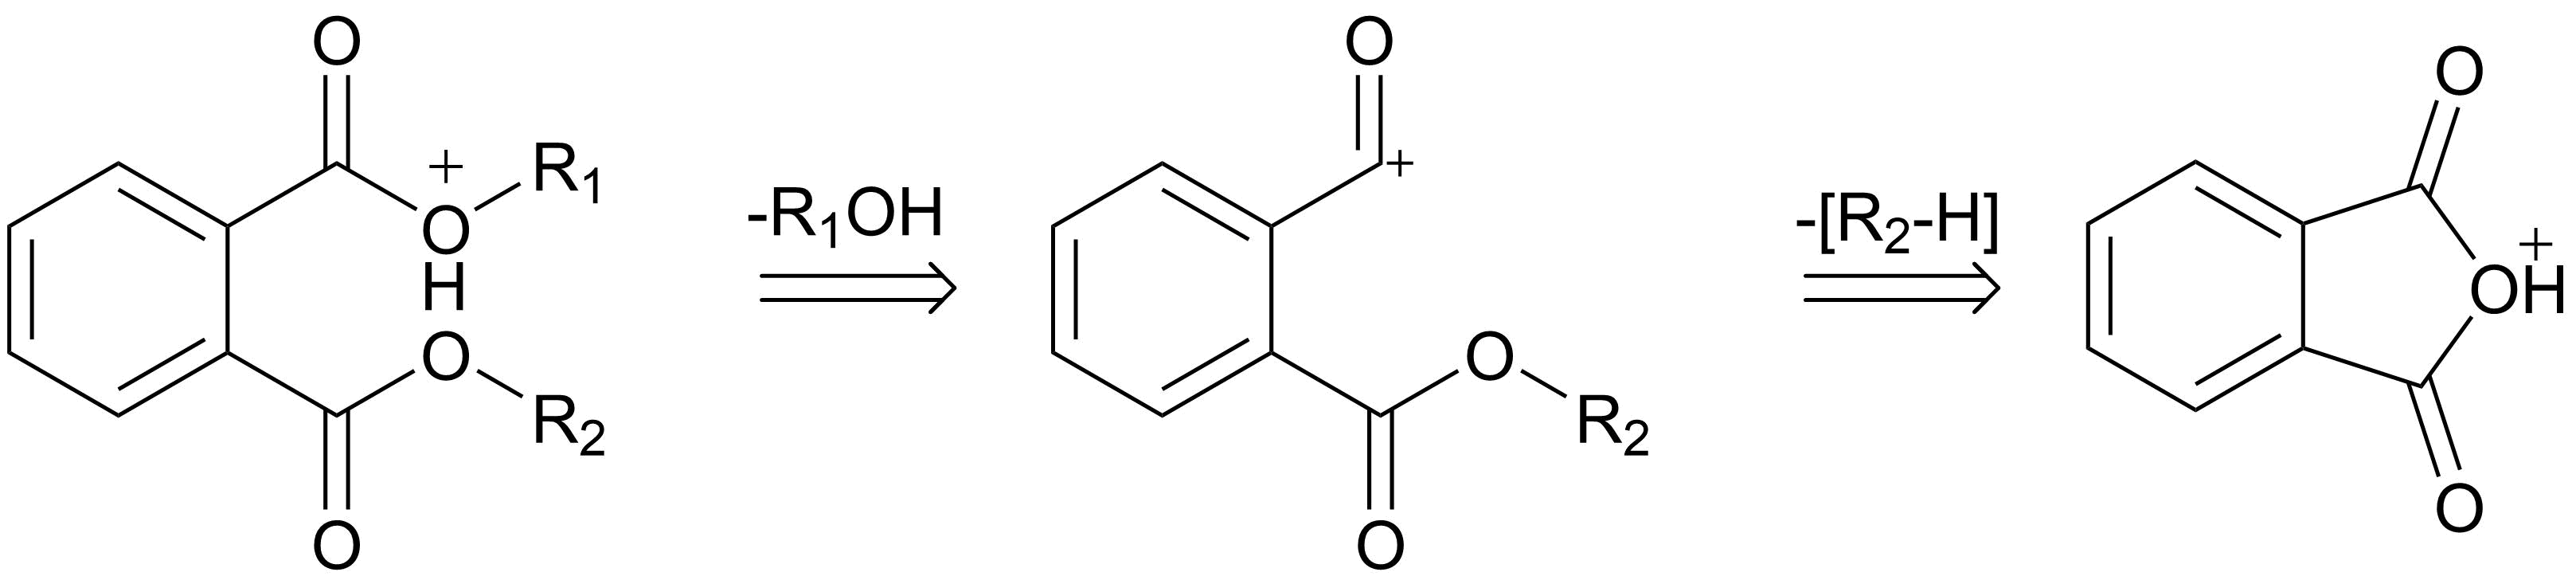
\includegraphics[height=0.12\textheight]{pics/PH/frag.png}
\caption{General fragmentation pathway from the protonated parent to  protonated phthalic anhydride at \textit{m/z} 149. Note that the neutrals molecules are omitted.}
\label{fig:PH_fr}
\end{figure}





\subsection{Phthalic acid}

\autoref{fig:PH_PAcid} shows the PID plot for the reaction of phthalic acid with the reagent ions as a function of the drift voltage and the reduced electric field. 
%
Only two product ions were observed: the protonated parent molecule  ((C$_8$H$_6$O$_4$)H$^+$)  at \textit{m/z} 167 and  protonated phthalic anhydride (C$_8$H$_{5}$O$_3^+$) at \textit{m/z} 149.
%
The latter is a characteristic phthalate product ion and is observed with many of these compounds.

    \begin{figure}[htb]
    \centering
    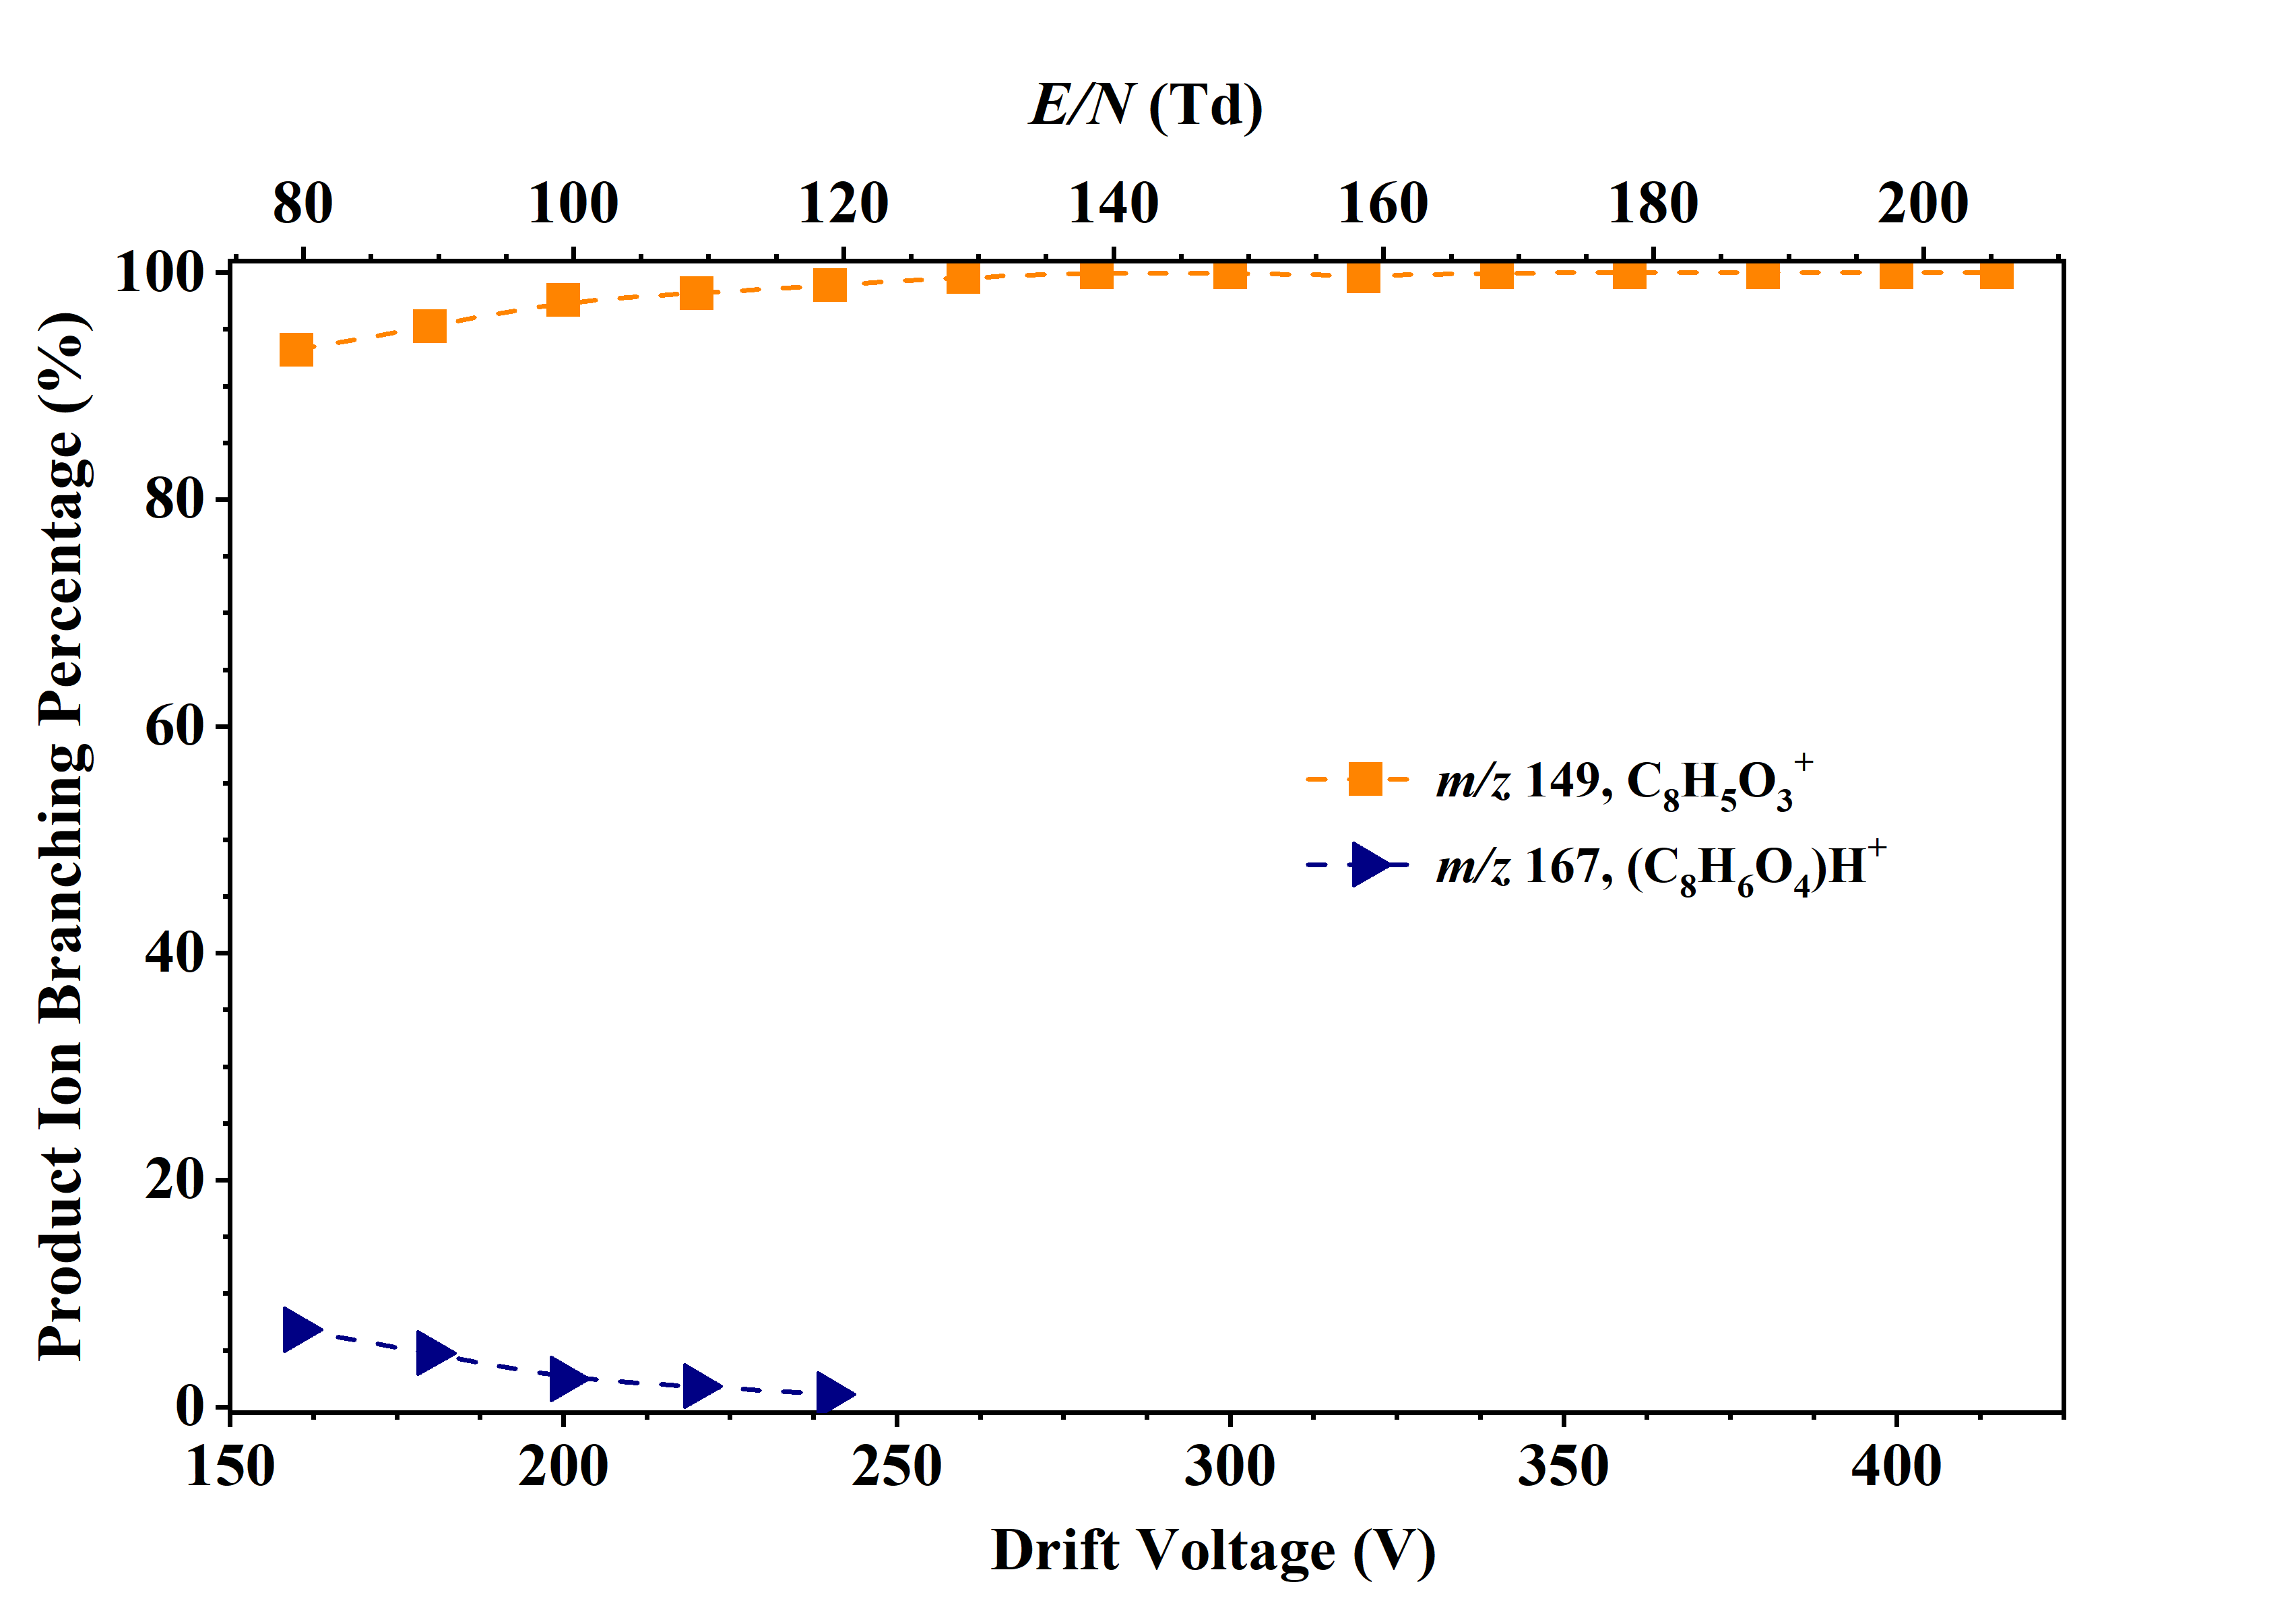
\includegraphics[height=0.4\textheight]{pics/Pacid-BR.png}
    \caption{Percentage product ion distribution resulting from the reaction of phthalic acid with (H$_2$O)$_n$H$_3$O$^+$ (n = 0, 1) as a function of the drift voltage and the reduced electric field in the range from 80 to 205 Td.}
    \label{fig:PH_PAcid}
    \end{figure}


The fact that these product ions resemble the reagent ions in \autoref{fig:PH_RI} indicates that the protonated parent ion is a product of the non-dissociative reaction of phthalic acid with (H$_2$O)H$_3$O$^+$, which is only found at trace levels at low \textit{E/N}.
%
Proton transfer from (H$_2$O)H$_3$O$^+$ is  softer  than that from H$_3$O$^+$, with a difference in gas basicity  of 124 kJ mol$^{-1}$ or 1.285 eV.
%
Even though there are not DFT results available to illustrate the loss of H$_2$O from protonated phthalic acid to give protonated phthalic anhydride, it can be concluded that this process is energetically favourable because the ion at \textit{m/z} 149 is observed for all \textit{E/N} values. 
%
The formation of this ion needs  protonation of one of the hydroxy oxygen atoms, which is a similar pathway to that of benzoic acid to yield benzoyl$^+$ (see section \ref{section:BzAcid}). %I am not sure about this









%This is in agreement with what was observed for the benzoate esters (which one?)



%This is a softer proton transfer reaction than that from H$_3$O$^+$, which yields the ion at \textit{m/z} 149.02. This corresponds to protonated phthalic anhydride (C$_8$H$_{5}$O$_3^+$) and it comes from the loss of water from the protonated parent molecule (\autoref{eq:PAcid}). 

%\begin{equation}
%PAcid + H_3O^+ \rightarrow (PAcidH^+)^* + H_2O \\
%(PAcidH^+)^*  \rightarrow [PAcid - H_2O]H^+ + H_2O
%%PAcid + H_3O^+ \rightarrow (PAcidH^+)^* + H_2O \rightarrow [PAcid - H_2O]H^+ + 2H_2O
%\label{eq:PAcid}
%\end{equation}

%Is this true? (by comparison with the benzoate esters):
%The loss of water  requires the proton to be on one of the two alkoxy oxygens while hydrogen bonded to the other one to yield a barrierless disociation, as it is observed for all the \textit{E/N} range (\textit{m/z} 149.02 roughly mirrors the PID of H$_3$O$^+$ in \autoref{fig:PH_RI} while \textit{m/z} 167.03 mirrors that of (H$_2$O)H$_3$O$^+$).






\subsection{Dimethyl phthalate}
DMP is the phthalate diester with the shortest alkyl chain. It is produced from phthalic anhydride and methanol, and  its main non-industrial application is as insect repellent for personal protection against biting insects  \cite{lowenheim1975industrial,o2013merck,brown1997insect}.


Dissociative proton transfer to yield C$_9$H$_{7}$O$_3^+$ at \textit{m/z} 163 after the loss of methanol from the protonated parent 
is the dominant channel for the reaction of DMP with H$_3$O$^+$ (\autoref{fig:PH_DMP_fs}).
The protonated parent ion, (C$_{10}$H$_{10}$O$_4$)H$^+$ at \textit{m/z} 195, only represents ca. 25\% of the total product ion signal at around 80 Td and it steadily decreases as the \textit{E/N} increases.
%
Interestingly, it was found that DMP is the only one of the alkyl diester phthalates studied here in which protonated phthalic anhydride is not a product ion, which agrees with the results from other techniques in the literature \cite{yin2014mass}.
%
The formation of protonated phthalic anhydride would require the further loss of the remaining methyl group in the ion observed at \textit{m/z} 163.
%
This is comparable to the ion with \textit{m/z} 123 being observed with all the benzoates except with methyl benzoate (see section \ref{section:MeBz}). 



\begin{figure}[htb]%[htbp]
\centering
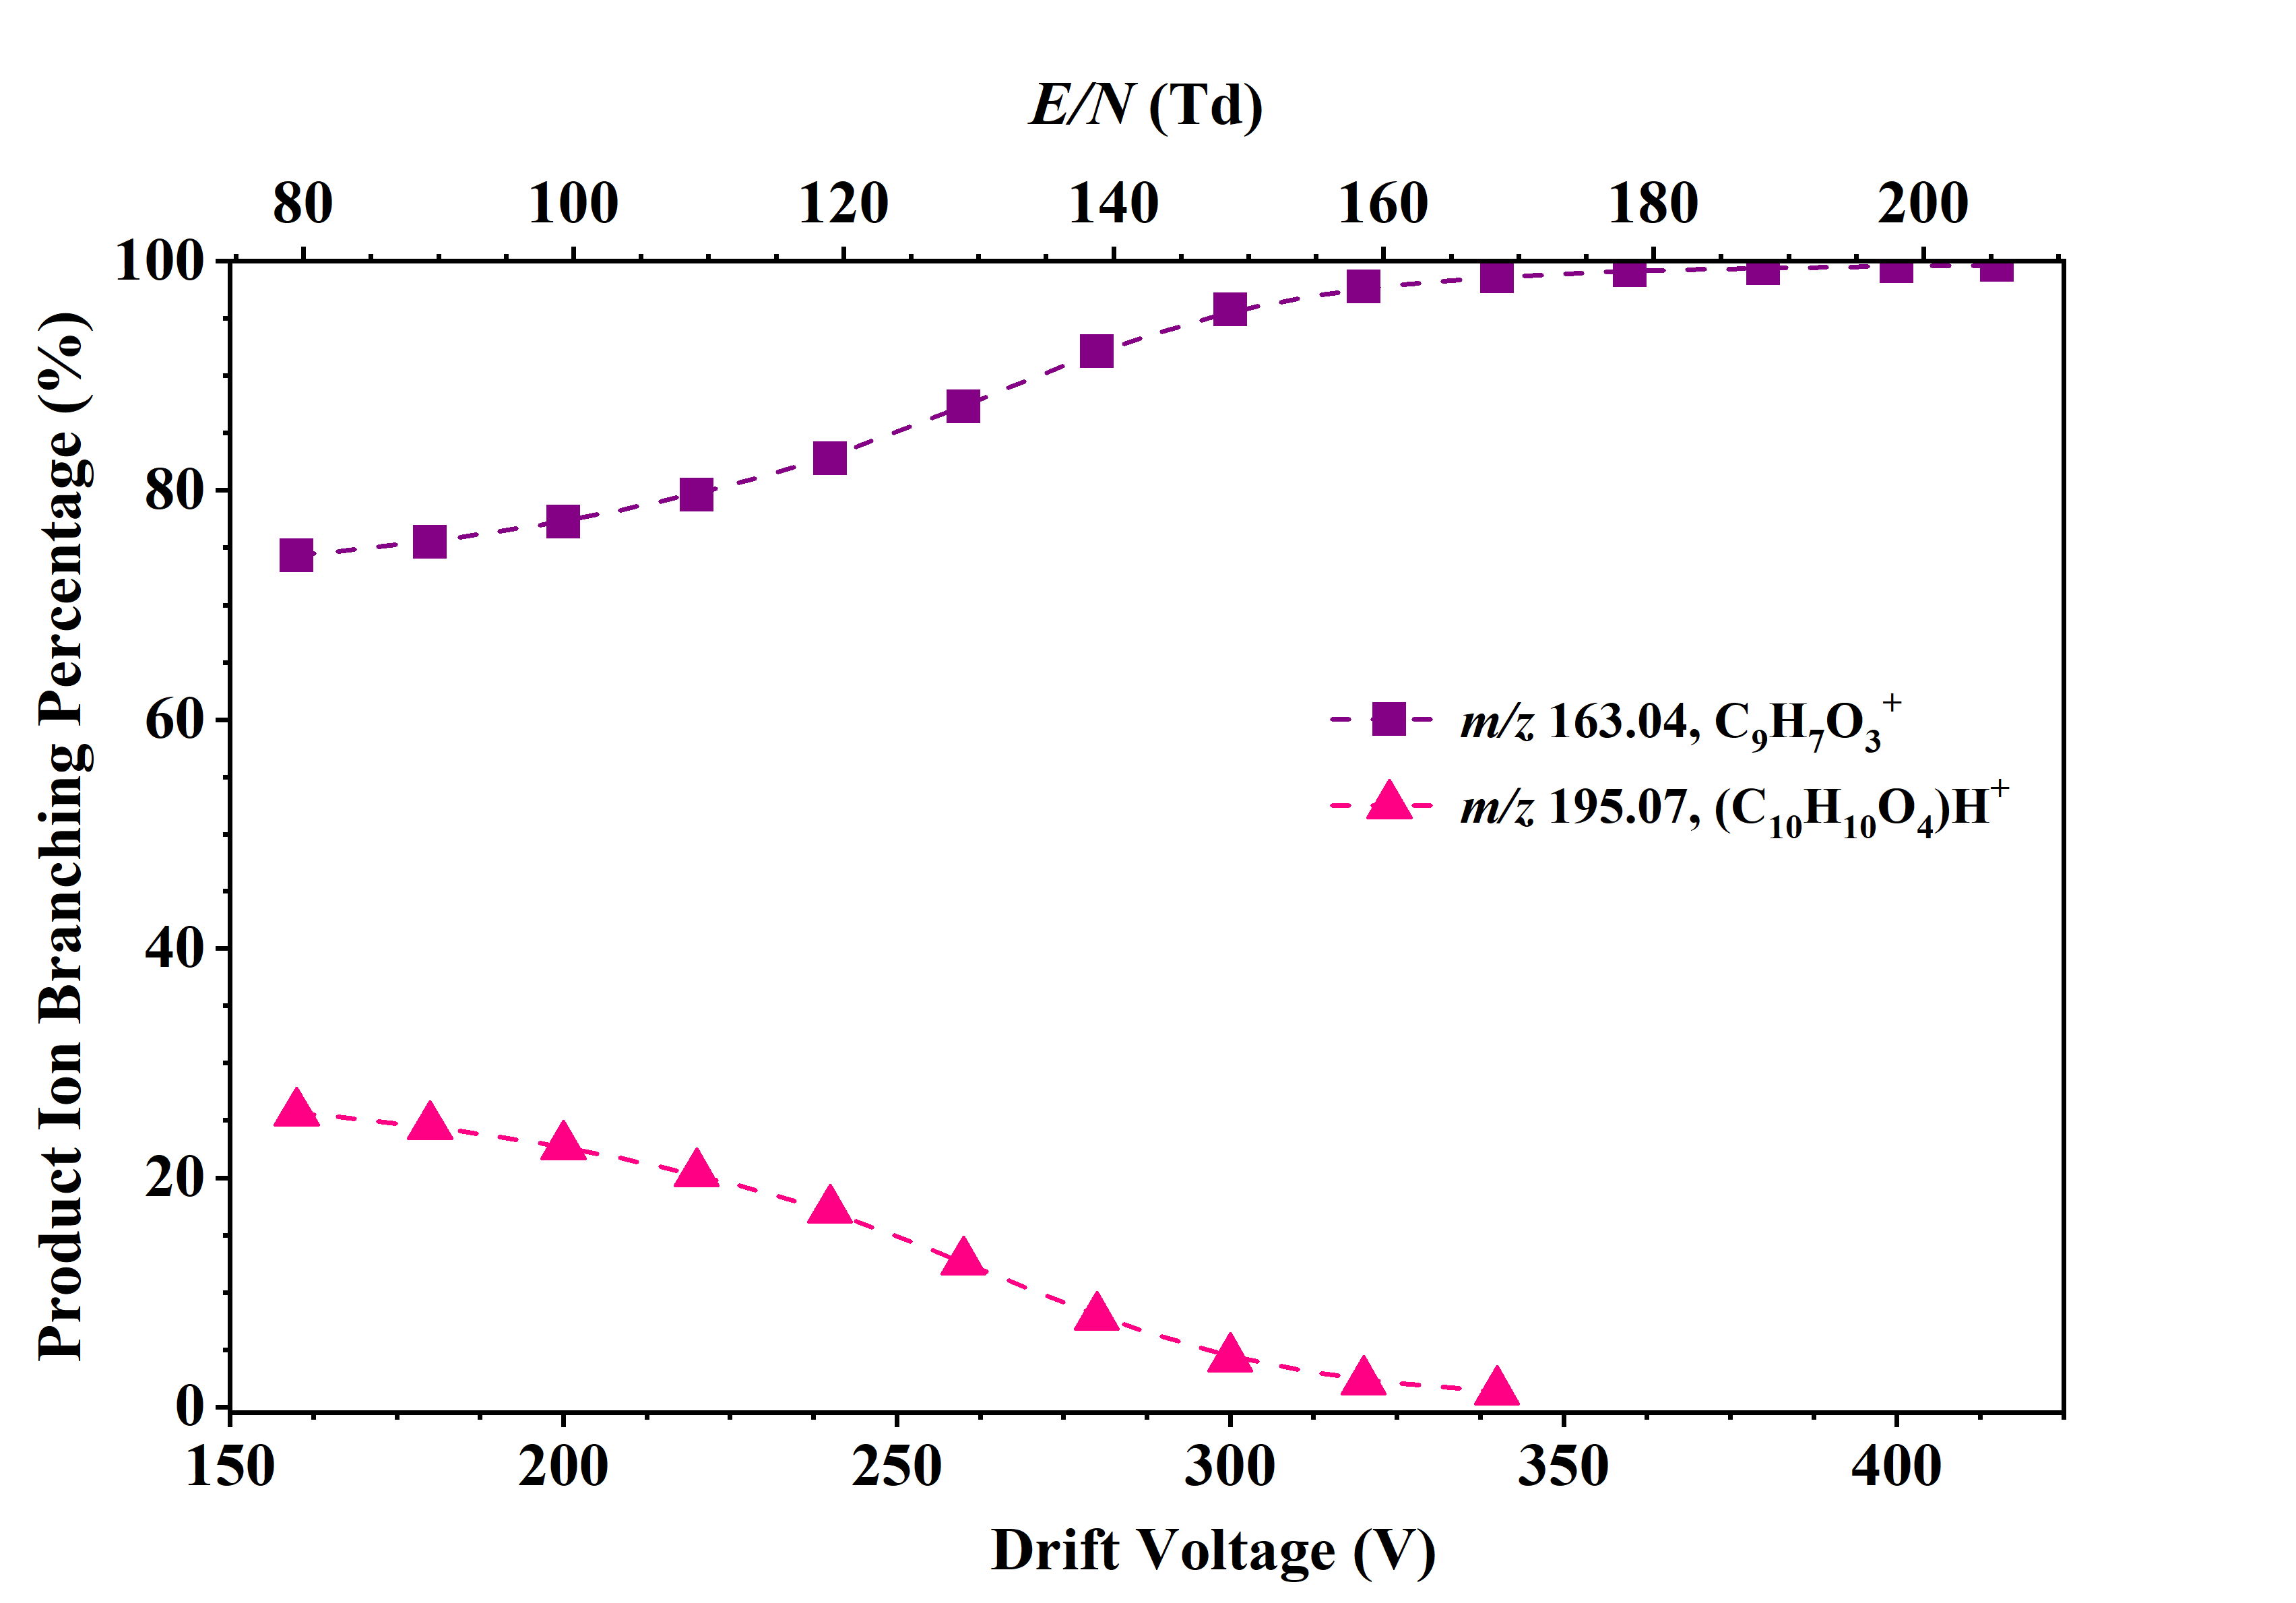
\includegraphics[height=0.4\textheight]{pics/DMP-BR.png}
\caption{Percentage product ion distribution resulting from the reaction of DMP with H$_3$O$^+$ as a function of the drift voltage and the reduced electric field in the range from 80 to 205 Td.}
\label{fig:PH_DMP_fs}
\end{figure}

%\begin{figure}[htb]%[htbp]
%\centering
%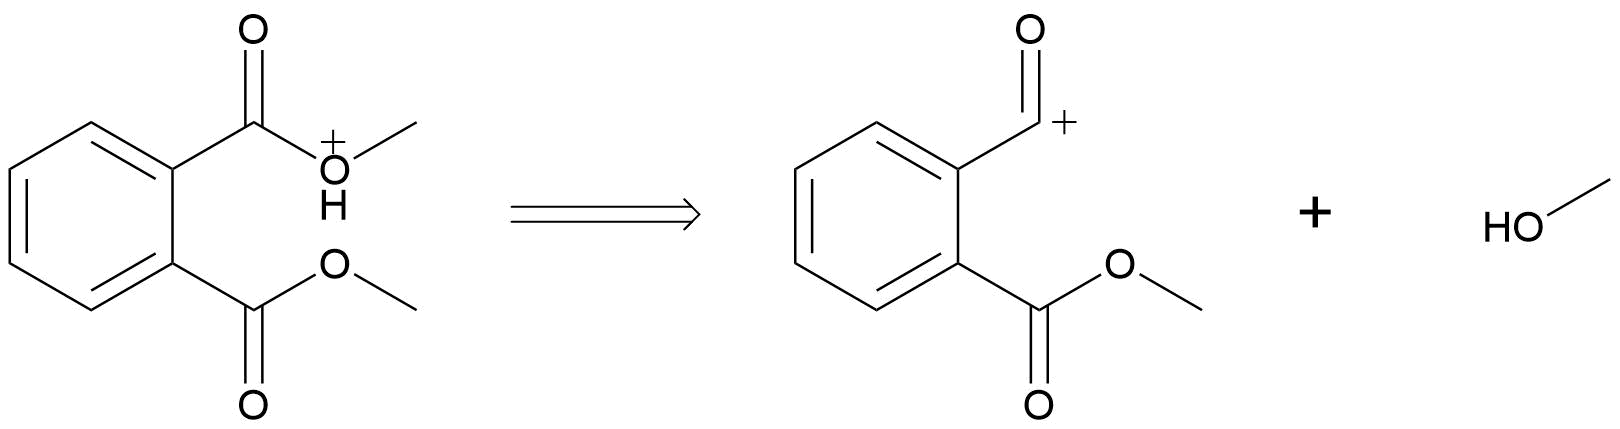
\includegraphics[height=0.1\textheight]{pics/PH/DMP_frag.png}
%\caption{DMP fragmentation pathway from the protonated parent to C$_9$H$_{7}$O$_3^+$ at \textit{m/z} 163. . Note that the neutrals molecules are omitted.}
%\label{fig:PH_DMP_fr}
%\end{figure}



\subsection{Diethyl phthalate}


\autoref{fig:PH_DEP_fs} shows the PID plot for the reaction of DEP with H$_3$O$^+$ as a function of the drift voltage and the reduced electric field.
At low \textit{E/N}, the most abundant ion at ca. 60\% is the protonated parent molecule, (C$_{12}$H$_{14}$O$_4$)H$^+$  at \textit{m/z} 223, which steadily decreases as the reduced electric field increases.
%
Another product ion is found at low \textit{E/N} at \textit{m/z} 75 and it is tentatively assigned to protonated ethyl formate (C$_3$H$_{7}$O$_2^+$).
The ion at \textit{m/z} 177, assigned to C$_{10}$H$_{9}$O$_3^+$, comes from the loss of ethanol from the protonated parent molecule and it peaks at around 150 Td with ca. 65\% of the total product ion signal.
At high \textit{E/N}, the dominant ion is protonated phthalic anhydride (C$_8$H$_{5}$O$_3^+$), formed through collision-induced dissociation, going up to 95\%. % for \textit{E/N} higher than 200 Td.
%
The MS$^2$ scan for the fragmentation of the MH$^+$ ion in the mzCloud database for diethyl phthalate agrees with the PTR-MS results in \autoref{fig:PH_DEP_fs} for higher \textit{E/N} than approximately 160 Td, although the protonated parent is not reported there while in the present PTR-MS experiments this ion represents ca. 10\% of the total ion signal at 160 Td
\cite{mzcloudDEP}.


\begin{figure}[htb]%[htbp]
\centering
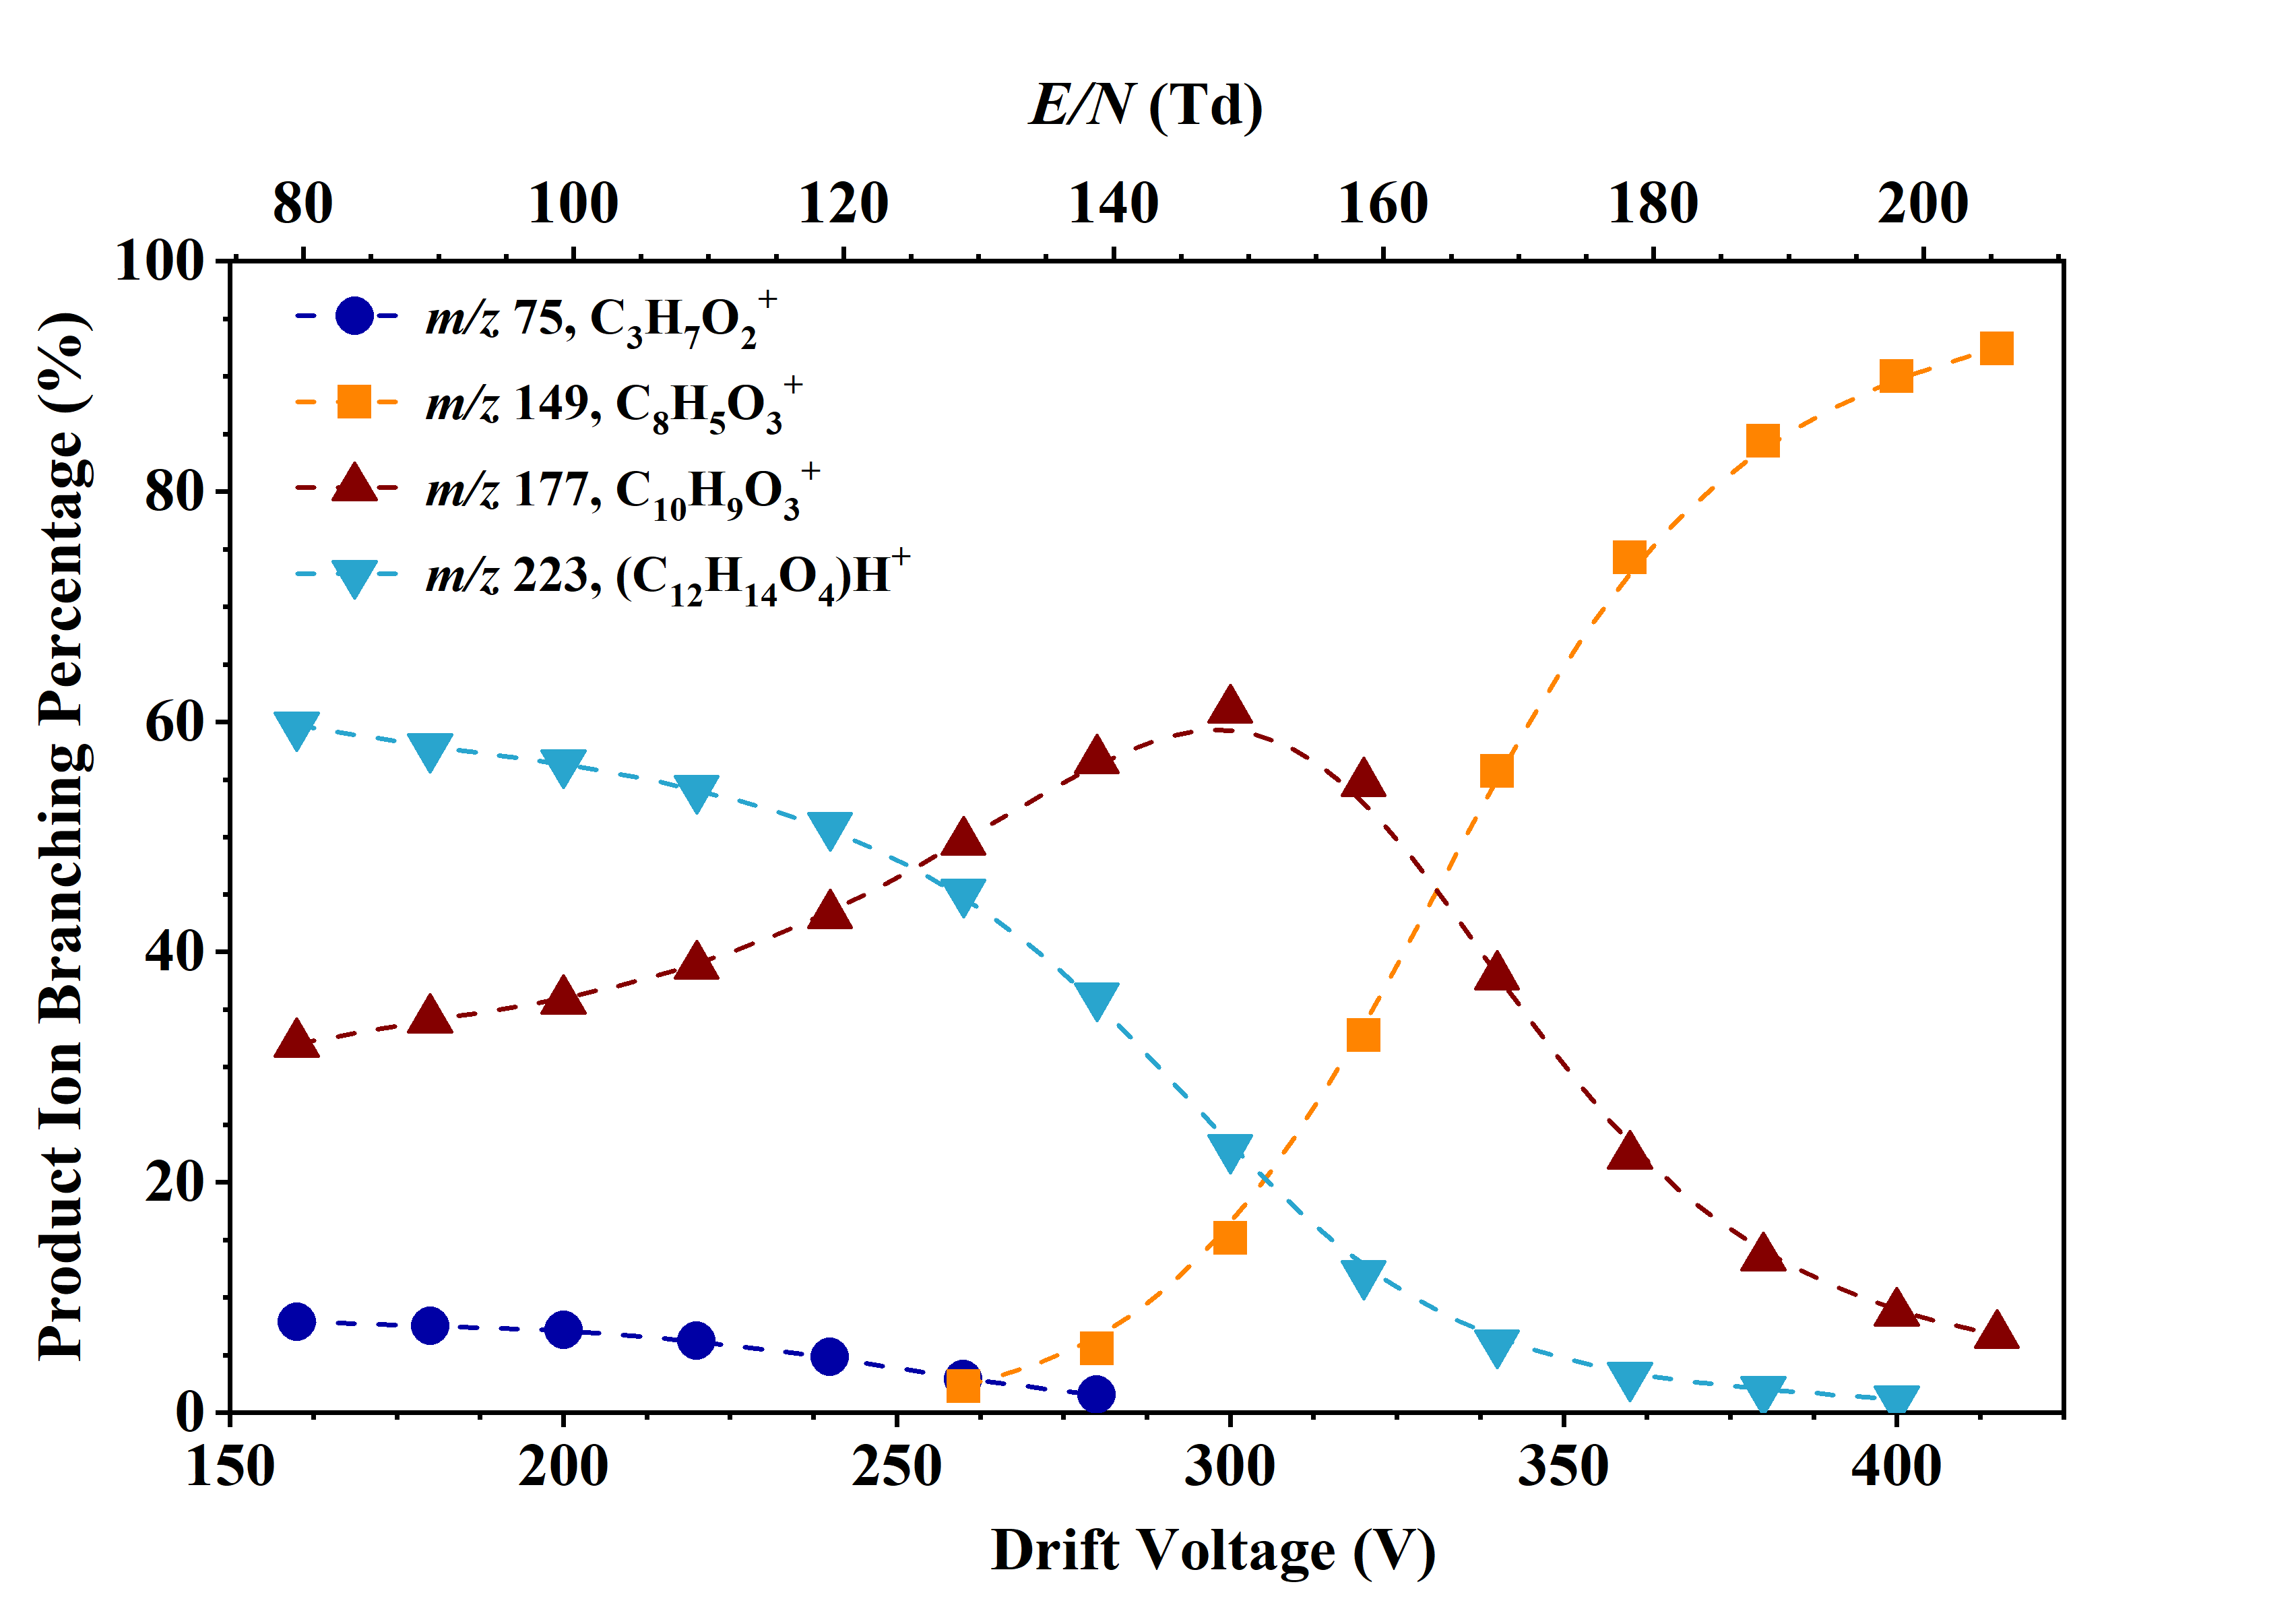
\includegraphics[height=0.4\textheight]{pics/DEP-BR.png}
\caption{Percentage product ion distribution resulting from the reaction of DEP with H$_3$O$^+$ as a function of the drift voltage and the reduced electric field in the range from 80 to 205 Td.}
\label{fig:PH_DEP_fs}
\end{figure}


\begin{figure}[htb]%[htbp]
\centering
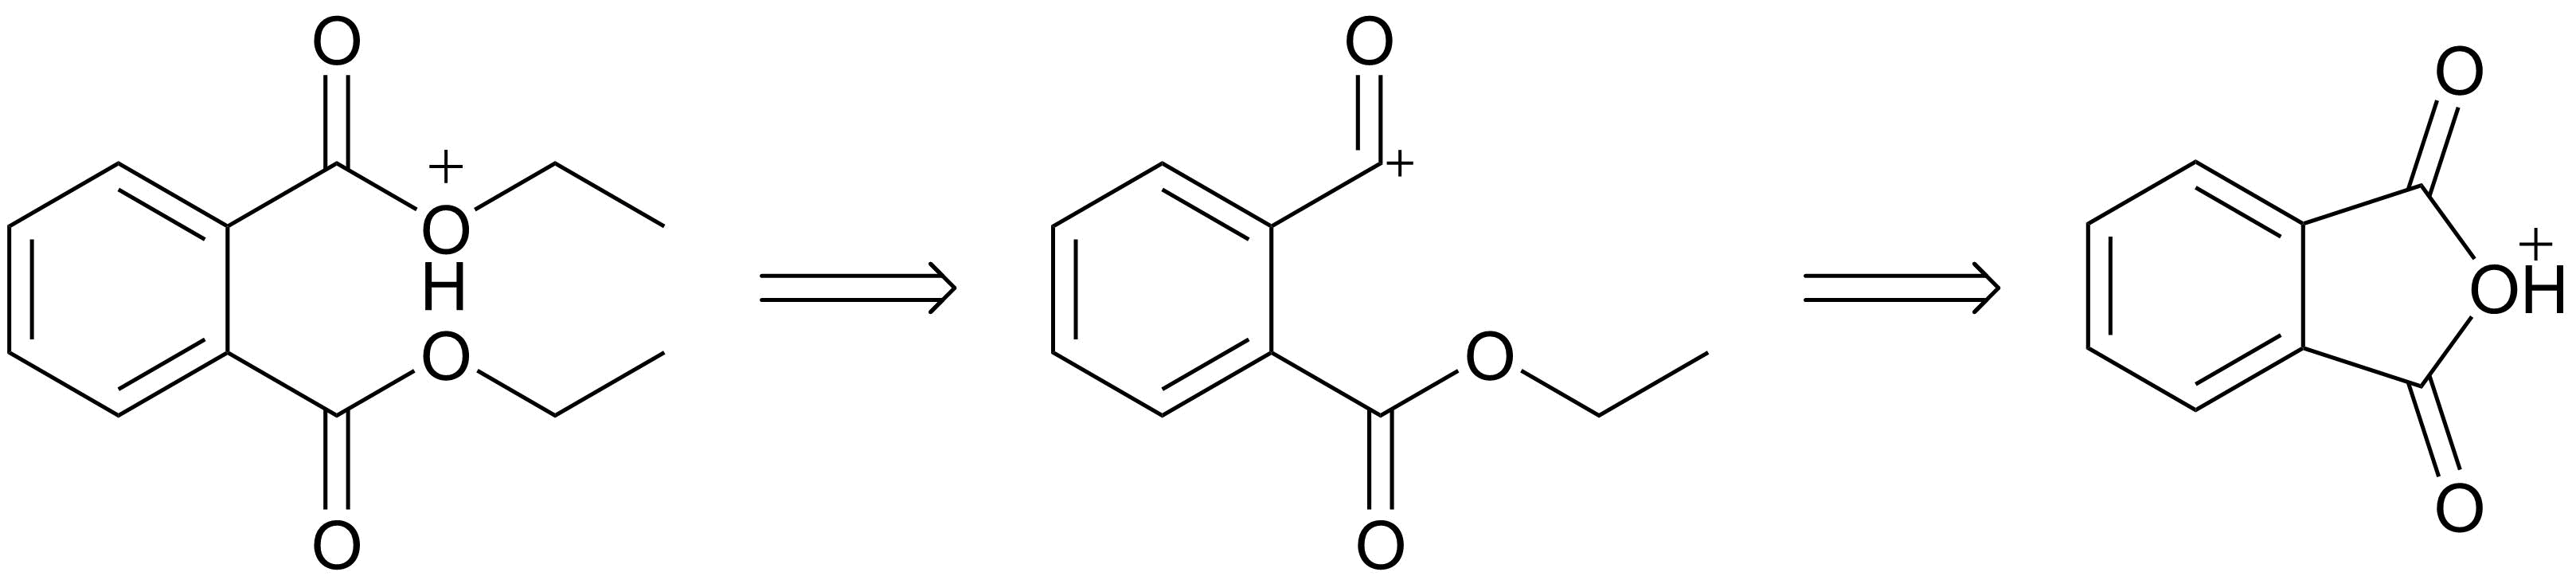
\includegraphics[height=0.1\textheight]{pics/PH/DEP_frag.png}
\caption{DEP fragmentation pathway from the protonated parent to the ions with \textit{m/z} 177 and \textit{m/z} 149 (i.e. protonated phthalic anhydride). Note that the neutrals molecules are omitted.}
\label{fig:PH_DEP_fr}
\end{figure}


\subsection{Diallyl phthalate}
DAP is a skin, eyes and mucous membranes irritant \cite{clayton1981patty}.
%
It is used in ........


Non-dissociative proton transfer to yield the protonated parent molecule, (C$_{14}$H$_{14}$O$_4$)H$^+$, at \textit{m/z} 247 is the dominant channel for the reaction of DAP with H$_3$O$^+$ from low reduced electric field up to around 150 Td (\autoref{fig:PH_DAP_fs}). Then the ion resulting from the loss of allyl alcohol (C$_{11}$H$_9$O$_3^+$ at \textit{m/z} 189) becomes dominant. At high \textit{E/N} we observe C$_3$H$_5^+$, tentatively assigned to  the allyl radical,  and C$_3$H$_3^+$.
%
These ions are produced in a cascade-like fragmentation pathway as the collisional energy increases.
%
However, another ion (i.e. C$_6$H$_9^+$ at \textit{m/z} 81) is observed over all the studied \textit{E/N} range.
%
Although its formation and structure are not clear yet, it has been reported at trace levels in the mzCloud database \cite{mzcloudDAP}.
%
One of its possible structures is protonated cyclohexadiene arising from the benzene core of the molecule, but this is hardly the correct one because this  is not observed with any other of the studied phthalates.
%
Another possibility would be that it comes from the two allyl (i.e. -CH$_2$CH=CH$_2$) branches but this is highly unlikely as in the most stable DAP conformer these branches are not close to each other.
%
Similarly to DMP, protonated phthalic anhydride was not observed in the DAP measurements.




\begin{figure}[htb]%[htbp]
\centering
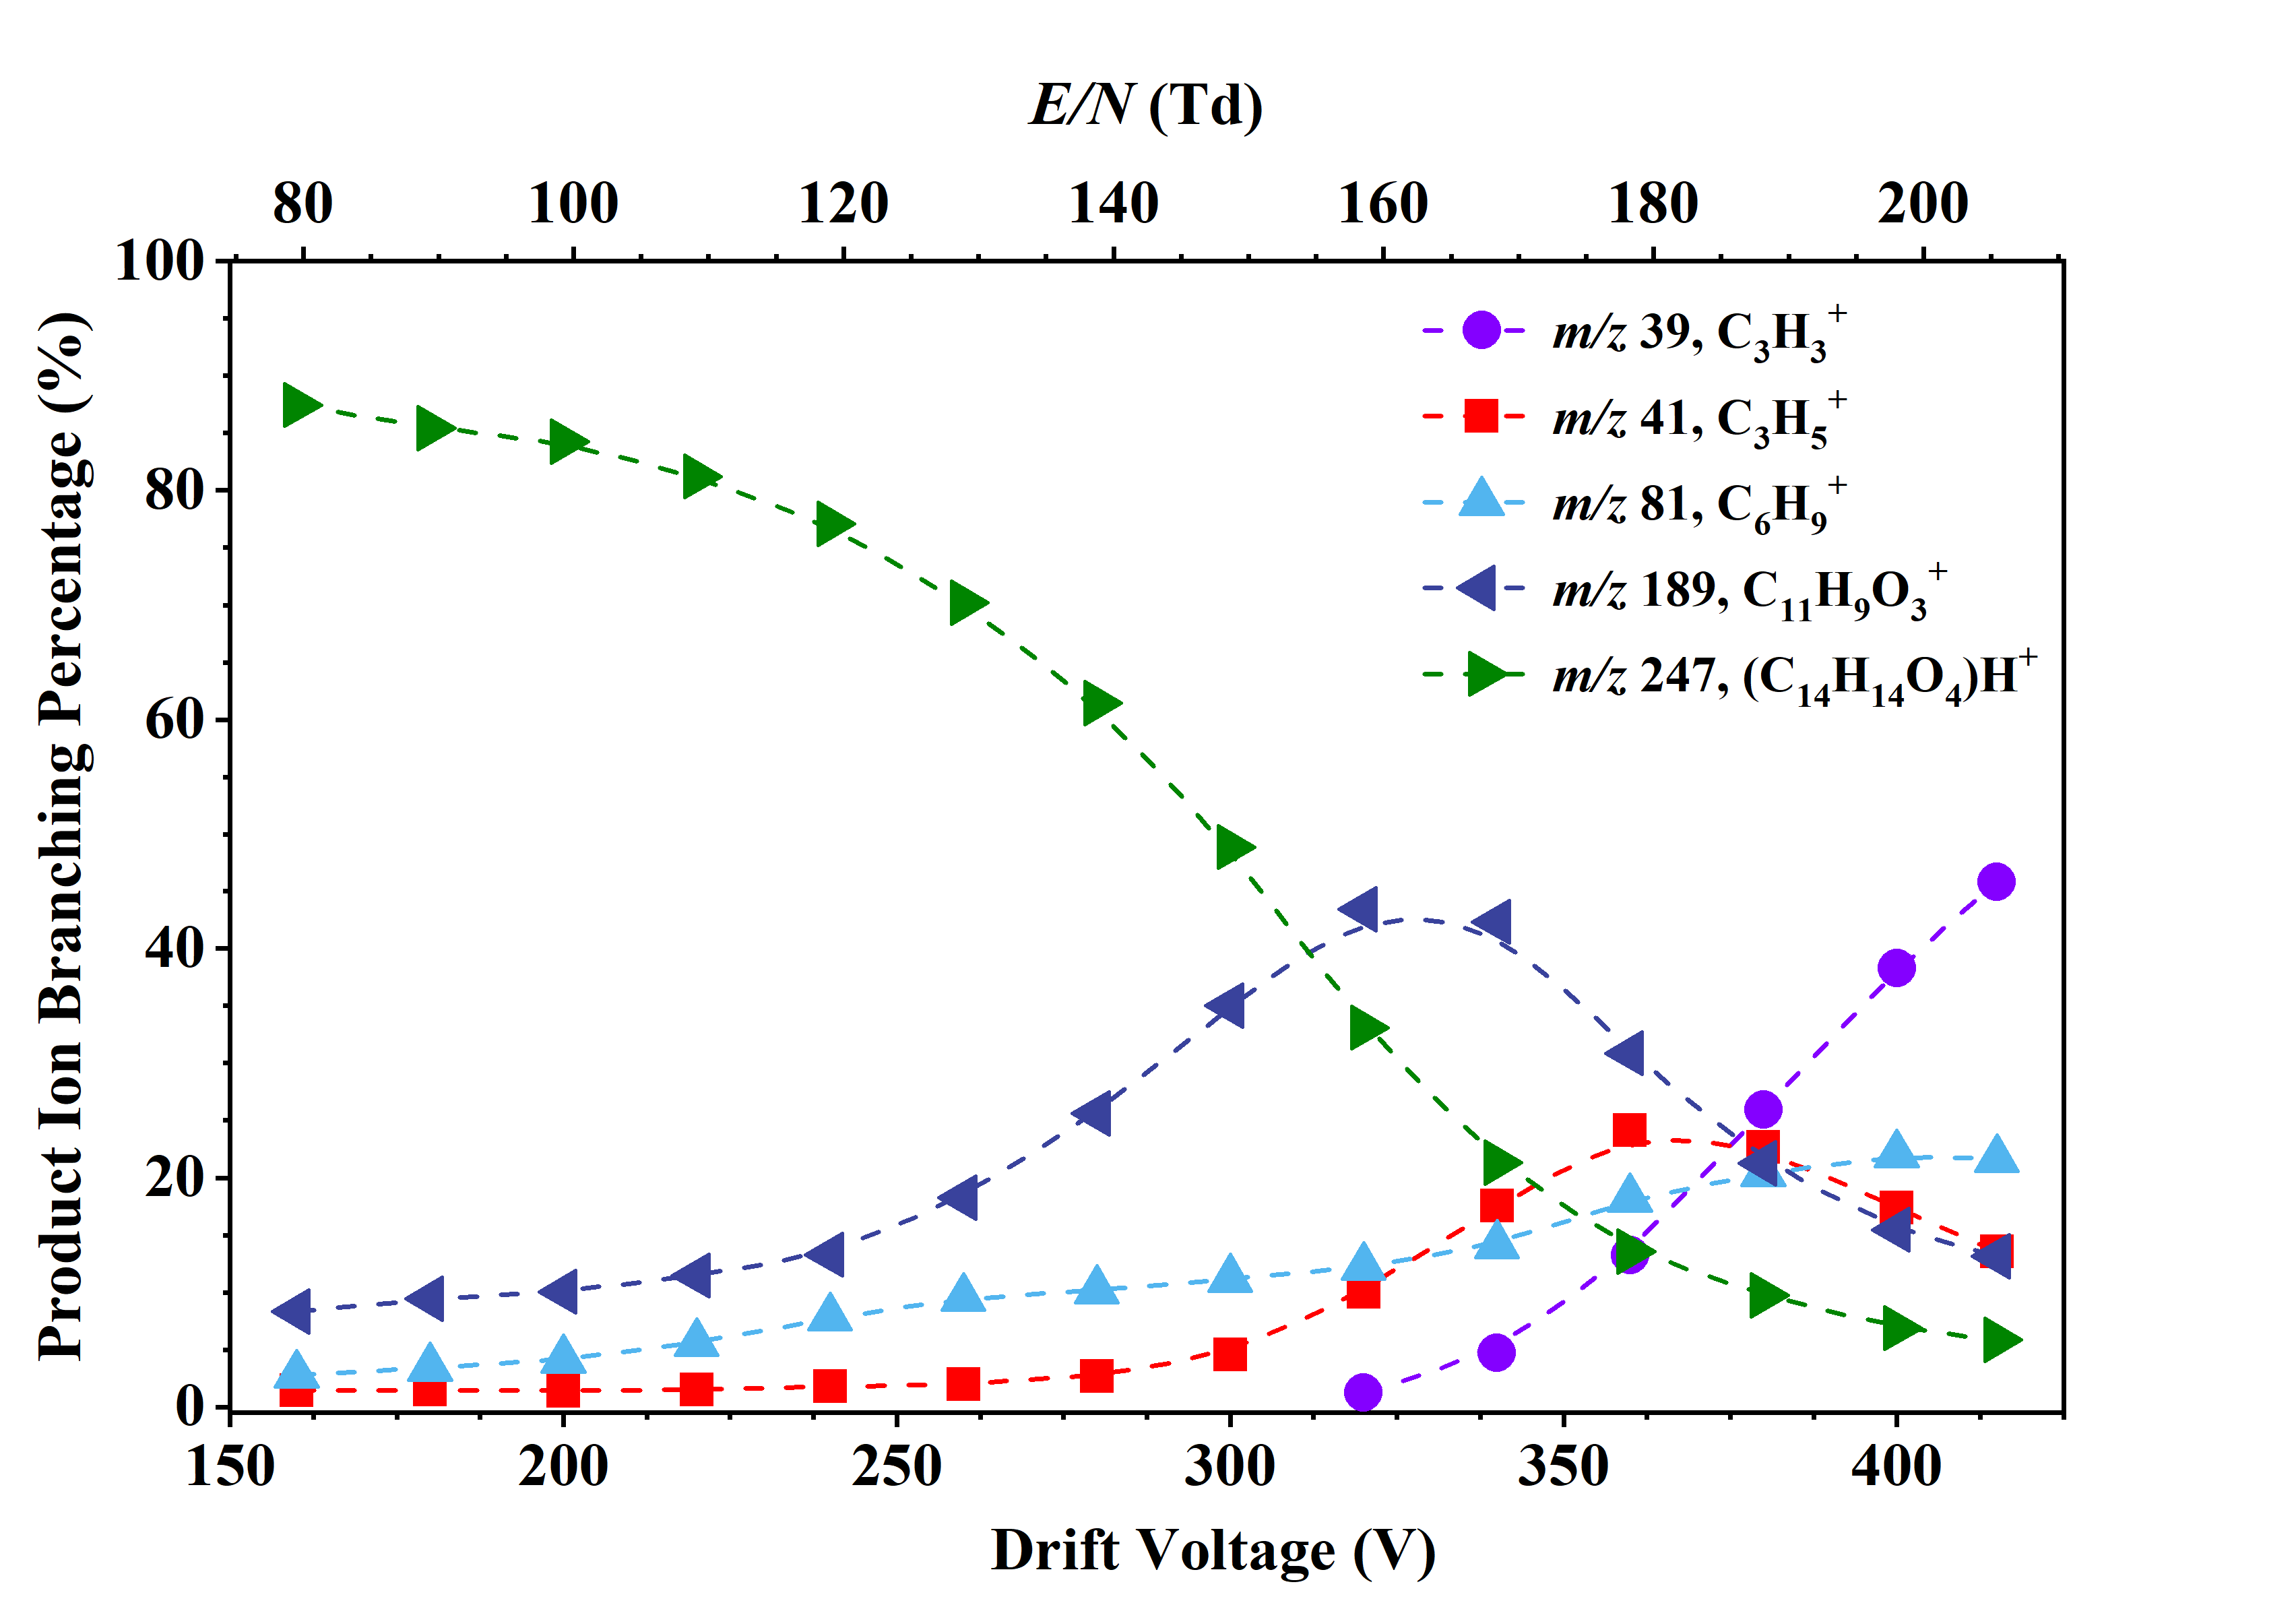
\includegraphics[height=0.4\textheight]{pics/DAP-BR.png}
\caption{Percentage product ion distribution resulting from the reaction of DAP with H$_3$O$^+$ as a function of the drift voltage and the reduced electric field in the range from 80 to 205 Td.}
\label{fig:PH_DAP_fs}
\end{figure}


\subsection{Dipropyl phthalate}


\autoref{fig:PH_DPP_fs} shows the PID for the reaction of H$_3$O$^+$ with DPP as a function of the reduced electric field in the range from 80 to 205 Td.
%
At low \textit{E/N}, the dominant ion is the protonated parent, (C$_{14}$H$_{18}$O$_4$)H$^+$, followed by the  loss of one of the propyl formate (i.e. C$_4$H$_6$O$_2$) branches from the protonated parent, yielding C$_{10}$H$_{13}$O$_2^+$, tentatively assigned to protonated propyl benzoate, and the loss of propanol from the protonated parent, yielding C$_{11}$H$_{11}$O$_3^+$. 
%
The abundance of these three ions decrease with the reduced electric field and at ca. 150 Td protonated phthalic anhydride becomes dominant.
%
The ions found at high \textit{E/N} are protonated benzoic acid (C$_{7}$H$_{7}$O$_2^+$) and  protonated benzene (C$_6$H$_{7}^+$).
A minor contribution is observed for the whole \textit{E/N} range from benzoyl$^+$ (C$_7$H$_{5}$O$^+$).

    \begin{figure}[htb]%[htbp]
    \centering
    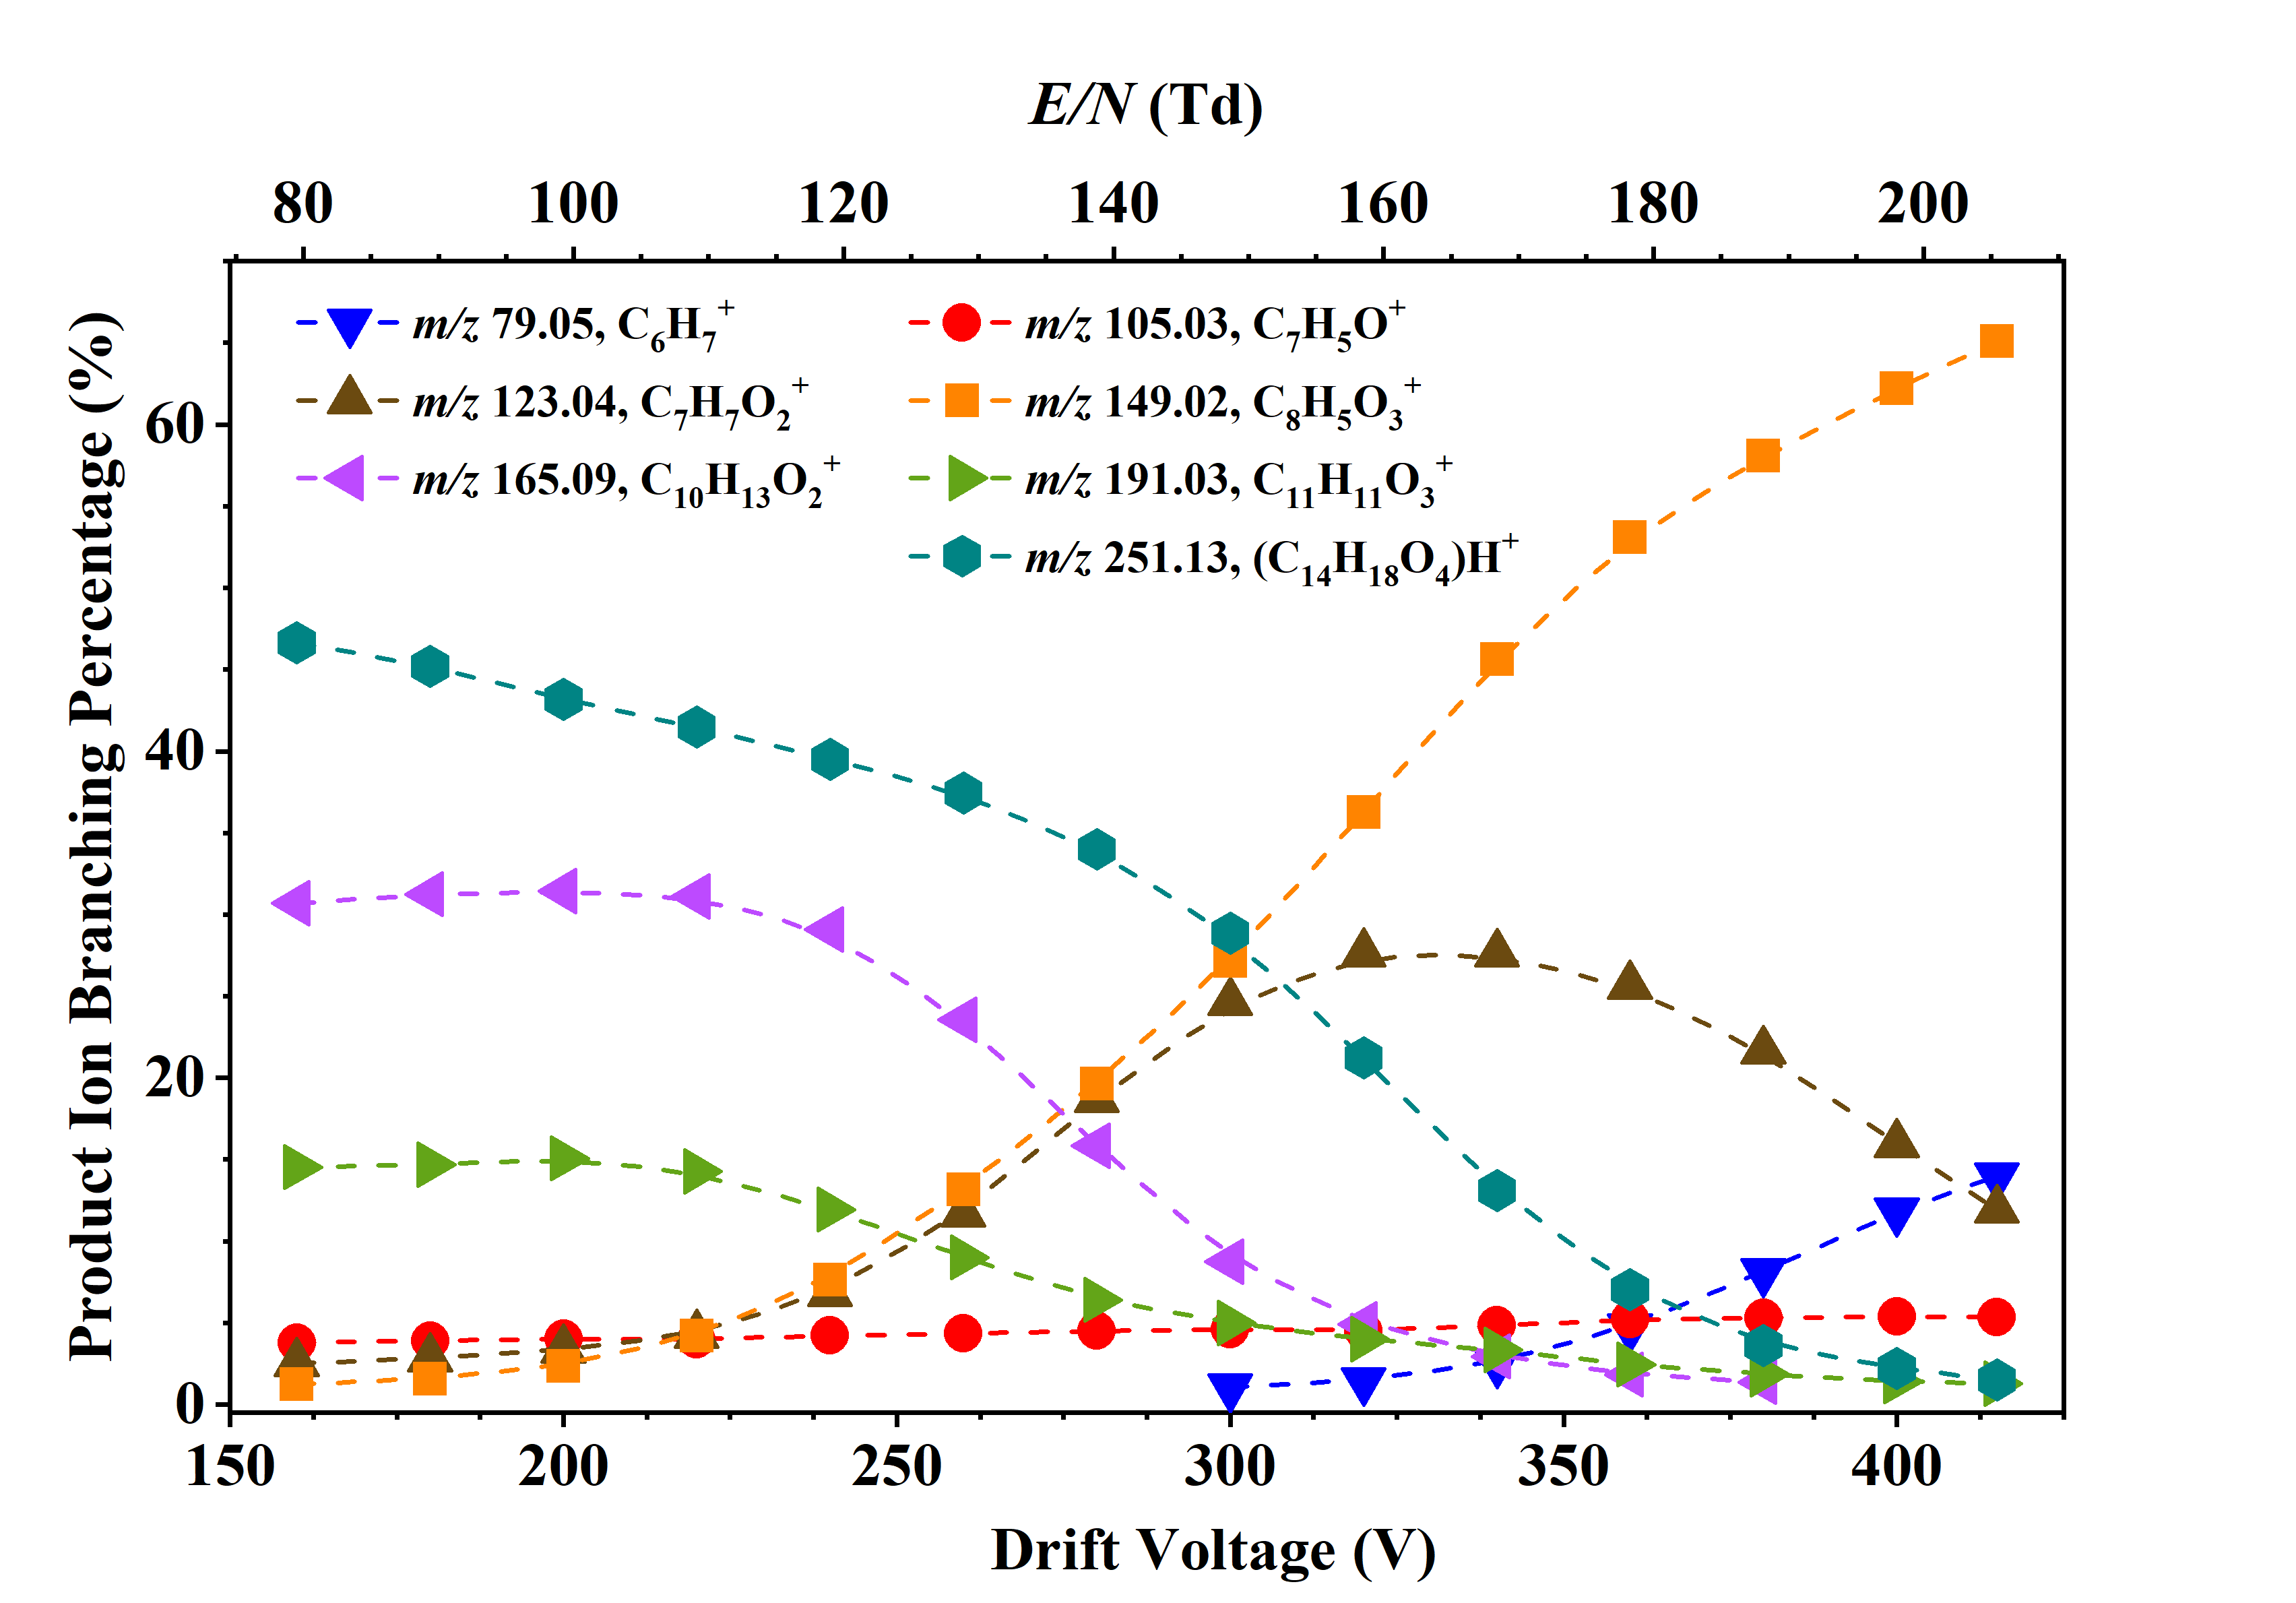
\includegraphics[height=0.4\textheight]{pics/DPP-BR.png}
    \caption{Percentage product ion distribution resulting from the reaction of DPP with H$_3$O$^+$ as a function of the drift voltage and the reduced electric field in the range from 80 to 205 Td.}
    \label{fig:PH_DPP_fs}
    \end{figure}
%




\subsection{Dibutyl phthalate}

%This is one of the most controlled and restricted phthalates in the EU, USA and  China.
%
The protonated parent ion  (C$_{16}$H$_{22}$O$_4$)H$^+$ at \textit{m/z} 279 is the most abundant ion from low \textit{E/N} up to around 130 Td, when protonated phthalic anhydride becomes the most abundant ion for the rest of the reduced electric field range (see \autoref{fig:PH_DBP_fs}).
%
At low \textit{E/N} we also found the  ion resulting from the loss of butanol from the protonated parent, C$_{12}$H$_{13}$O$_3^+$ at \textit{m/z} 205,  and the loss of butyl formate (i.e. C$_{5}$H$_{8}$O$_2$) to yield C$_{11}$H$_{15}$O$_2^+$ at \textit{m/z} 179, which is tentatively assigned to protonated butyl benzoate.
%
At high \textit{E/N} some minor ions are protonated benzoic acid (C$_{7}$H$_{7}$O$_2^+$), benzoyl$^+$ (C$_7$H$_{5}$O$^+$) and protonated benzene (C$_6$H$_{7}^+$) at \textit{m/z} 123, \textit{m/z} 105 and \textit{m/z} 79, respectively.


Tandem MS$^3$ spectra acquired by subsequently fragmenting the protonated parent at \textit{m/z} 279 and C$_{12}$H$_{13}$O$_3^+$ at \textit{m/z} 205 proves that the formation of protonated phthalic anhydride from protonated DBP can occur following the pathway described in \autoref{fig:PH_fr} \cite{mzcloudDBP}.
%



\begin{figure}[htb]%[htbp]
\centering
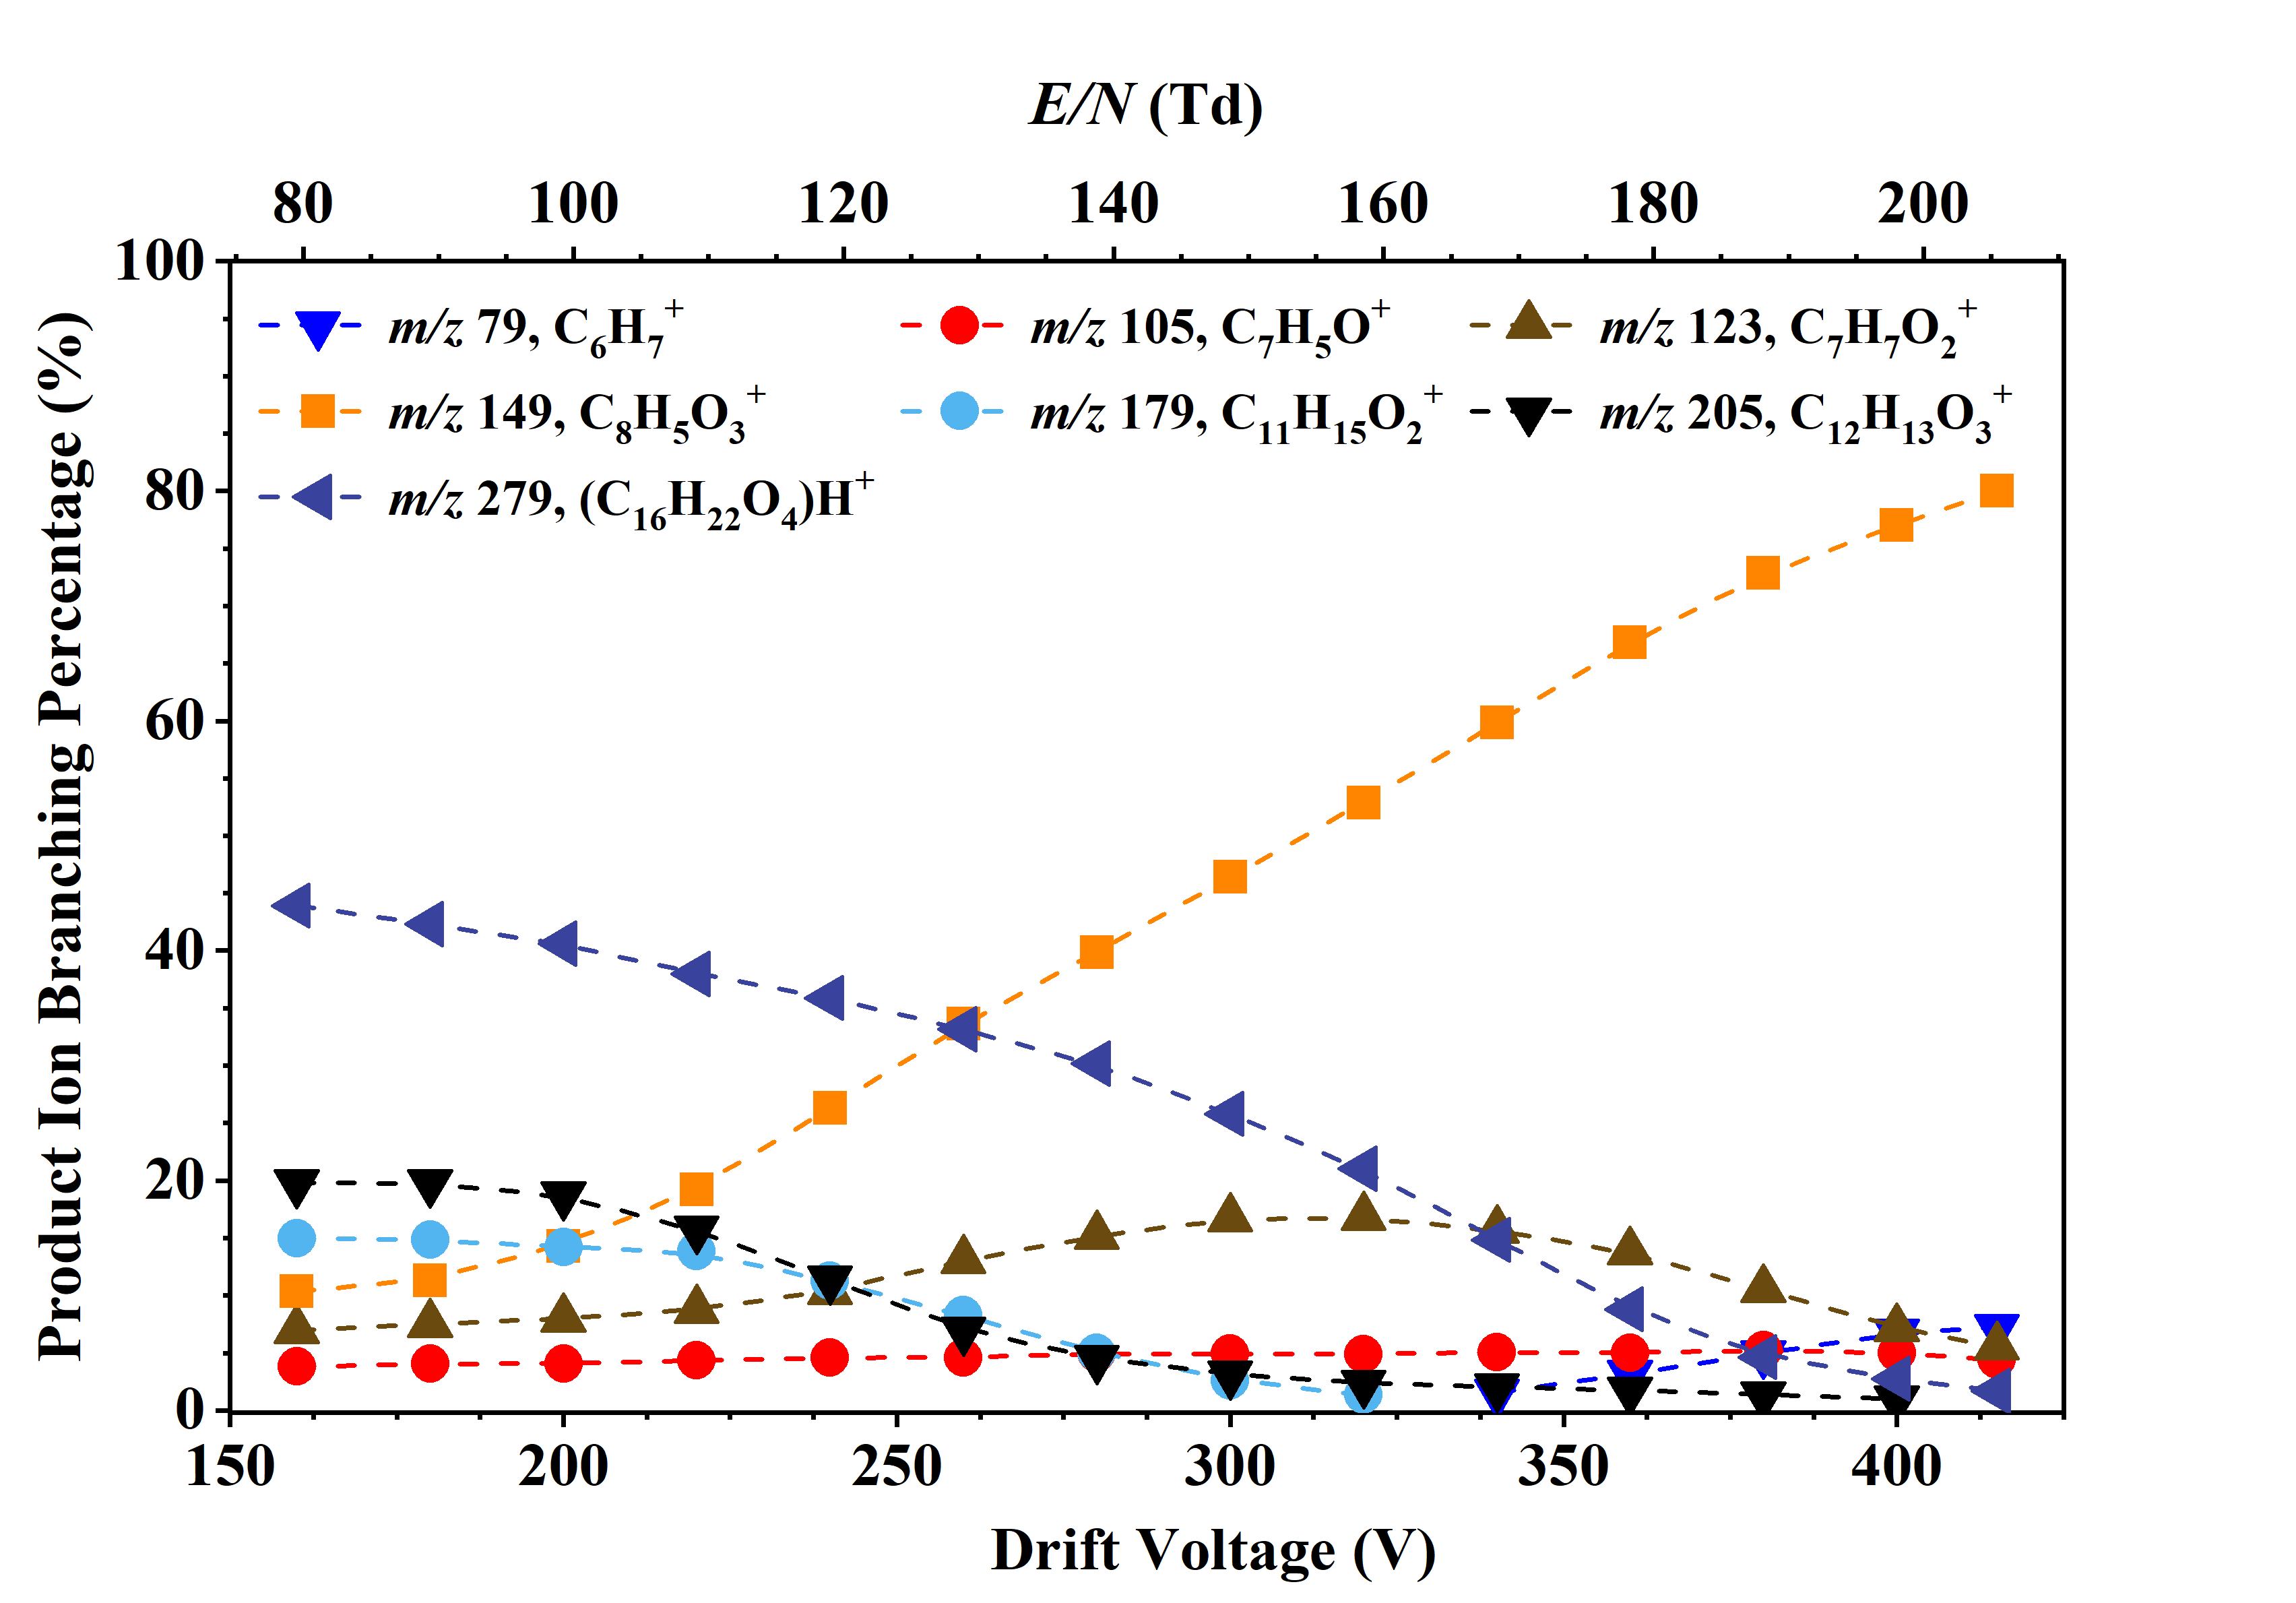
\includegraphics[height=0.4\textheight]{pics/DBP-BR.png}
\caption{Percentage product ion distribution resulting from the reaction of DBP with H$_3$O$^+$ as a function of the drift voltage and the reduced electric field in the range from 80 to 205 Td.}
\label{fig:PH_DBP_fs}
\end{figure}




\subsection{Monoethylhexyl phthalate}


This phthalate is an active metabolite of DEHP formed through hydrolysis. The detection of MEHP in urine of children has been linked to exposure to DEHP \cite{becker2004dehp}.


Protonated phthalic anhydride is the dominant ion for all the \textit{E/N} range (\autoref{fig:PH_MEHP_fs}) while the protonated parent (i.e. \textit{m/z} 279) was not observed for any reduced electric field value.
%
C$_8$H$_{17}$O$^+$ at \textit{m/z} 129 is tentatively assigned to protonated 2-ethylhexanal (structure shown in \autoref{fig:PH_MEHP_frag}) and all the other product ions potentially come from the successive fragmentation of this one:
C$_8$H$_{17}^+$ at \textit{m/z} 113,
C$_8$H$_{15}^+$ at \textit{m/z} 111,
C$_5$H$_{11}^+$ at \textit{m/z} 71,
C$_5$H$_9^+$ at \textit{m/z} 69,
C$_4$H$_9^+$ at \textit{m/z} 57,
C$_3$H$_7^+$ at \textit{m/z} 43,
C$_3$H$_5^+$ at \textit{m/z} 41
and
C$_3$H$_3^+$ at \textit{m/z} 39.

The parent ion was not observed either for positive ESI MS$^2$ spectra in the mzCloud database for MEHP even at the lowest collisional energies, while negative ESI MS$^2$ spectra shows that the deprotonated parent (i.e. \textit{m/z} 277) is the dominant ion up to ca. 11 eV \cite{mzcloudMEHP}.


%The fact that the parent ion is not observed agrees with the MS$^2$ spectra in the mzCloud database and the literature for the detection of MEHP in positive mode  although interestingly for the negative mode the deprotonated parent \textit{m/z} 277 was reported \cite{mzcloudMEHP}.






%the ion at \textit{m/z} 129.13 is C$_8$H$_{17}$O$^+$,
%the ion at \textit{m/z} 113.13 is C$_8$H$_{17}^+$,
%the ion at \textit{m/z} 111.12 is C$_8$H$_{15}^+$,  
%the ion at \textit{m/z} 71.09 is C$_5$H$_{11}^+$,
%the ion at \textit{m/z} 69.07 is C$_5$H$_9^+$,
%the ion at \textit{m/z} 57.07 is C$_4$H$_9^+$, 
%the ion at \textit{m/z} 43.05 is CC$_3$H$_7^+$,
%the ion at \textit{m/z} 41.04 is C$_3$H$_5^+$
%and
%the ion at \textit{m/z} 39.02 is C$_3$H$_3^+$. 

\begin{figure}[htb]%[htbp]
\centering
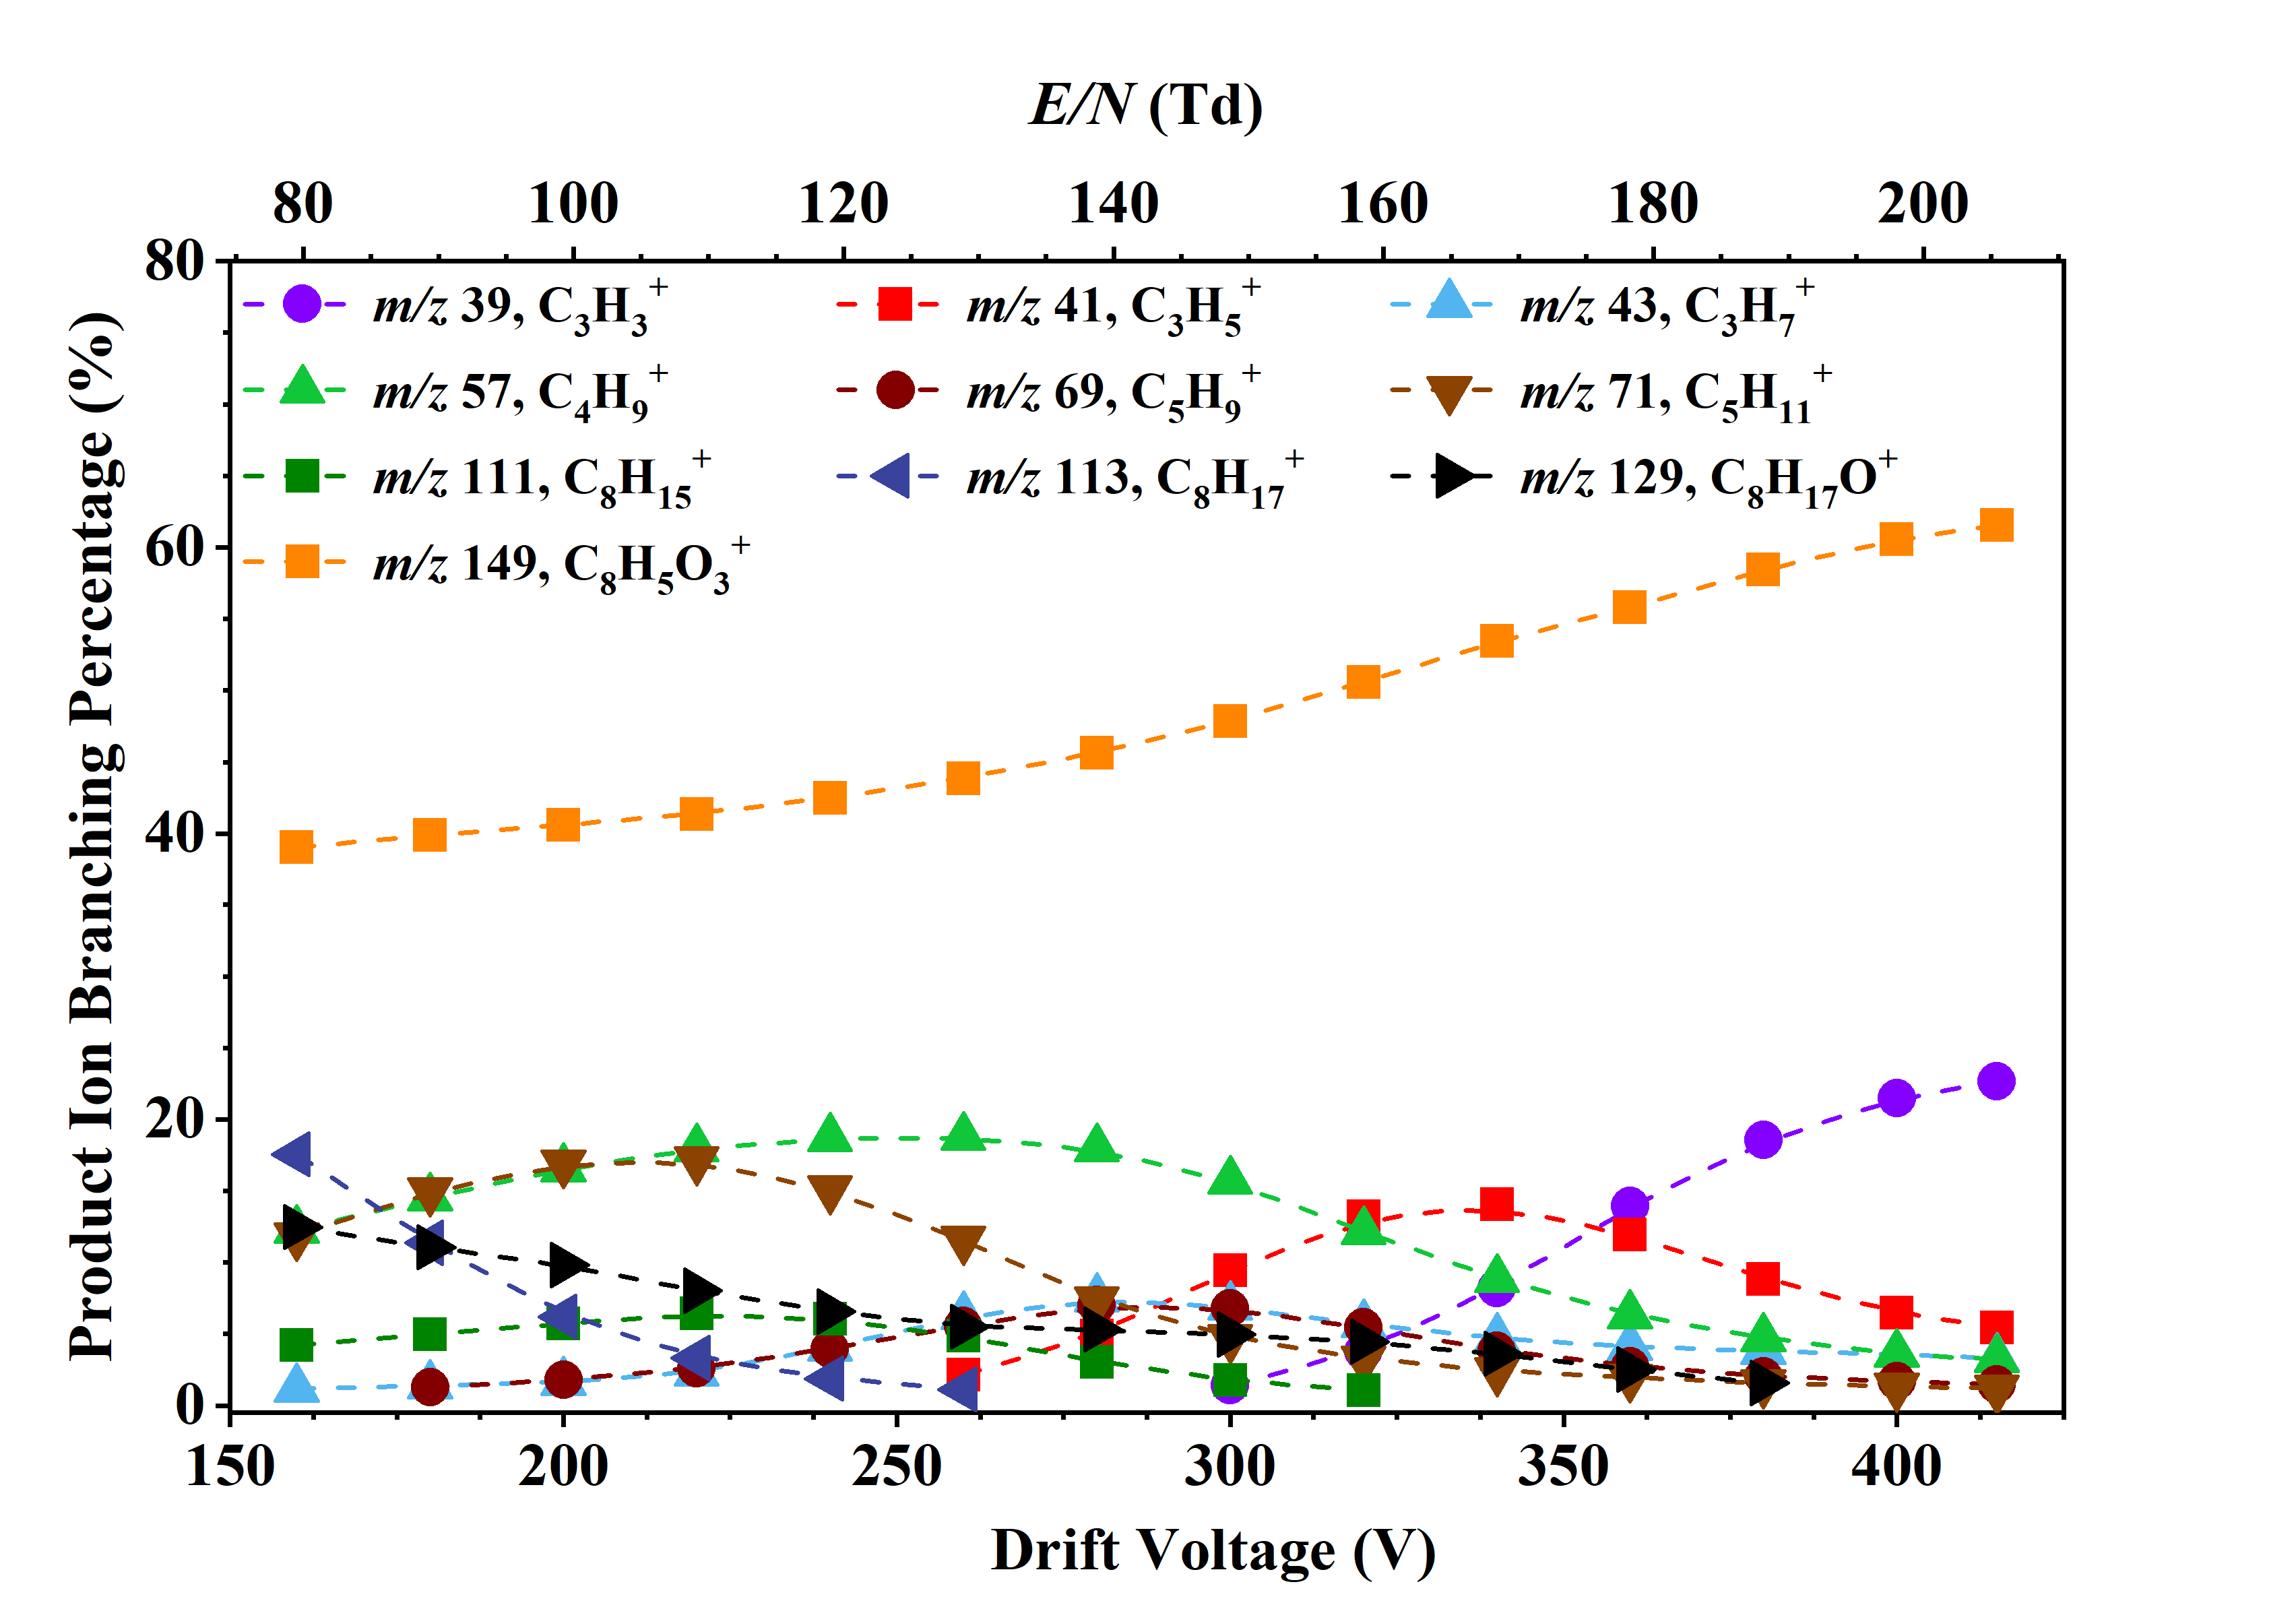
\includegraphics[height=0.4\textheight]{pics/MEHP-BR.png}
\caption{Percentage product ion distribution resulting from the reaction of MEHP with H$_3$O$^+$ as a function of the drift voltage and the reduced electric field in the range from 80 to 205 Td.}
\label{fig:PH_MEHP_fs}
\end{figure}


\begin{figure}[htb]%[htbp]
\centering
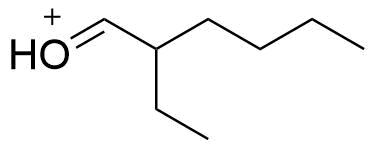
\includegraphics[height=0.05\textheight]{pics/PH/MEHP_frag.png}
\caption{Structure of protonated 2-ethylhexanal (i.e. C$_8$H$_{17}$O$^+$ at \textit{m/z} 129).}
\label{fig:PH_MEHP_frag}
\end{figure}


\subsection{Diisobutyl phthalate}

The PID of the reaction of DiBP with H$_3$O$^+$ (\autoref{fig:PH_DiBP_fs}) is comparable to that of its isomer DBP (\autoref{fig:PH_DBP_fs}) because the most relevant ions are the same but they appear at different  proportions.
The two dominant ions are as well the protonated parent molecule ((C$_{16}$H$_{22}$O$_4$)H$^+$ at \textit{m/z} 279) at lower \textit{E/N} and protonated phthalic anhydride at higher \textit{E/N}, but for DiBP the crossover point is at ca. 170 Td, instead of at ca. 130 Td as it occurs for DBP.
Another two product ions are observed:  C$_4$H$_9^+$ at \textit{m/z} 57 is tentatively assigned to isobutyl$^+$ and 
at low \textit{E/N} there are traces of the loss of isobutanol from the protonated parent molecule (C$_{12}$H$_{13}$O$_3^+$ at \textit{m/z} 205).




\begin{figure}[htb]%[htbp]
\centering
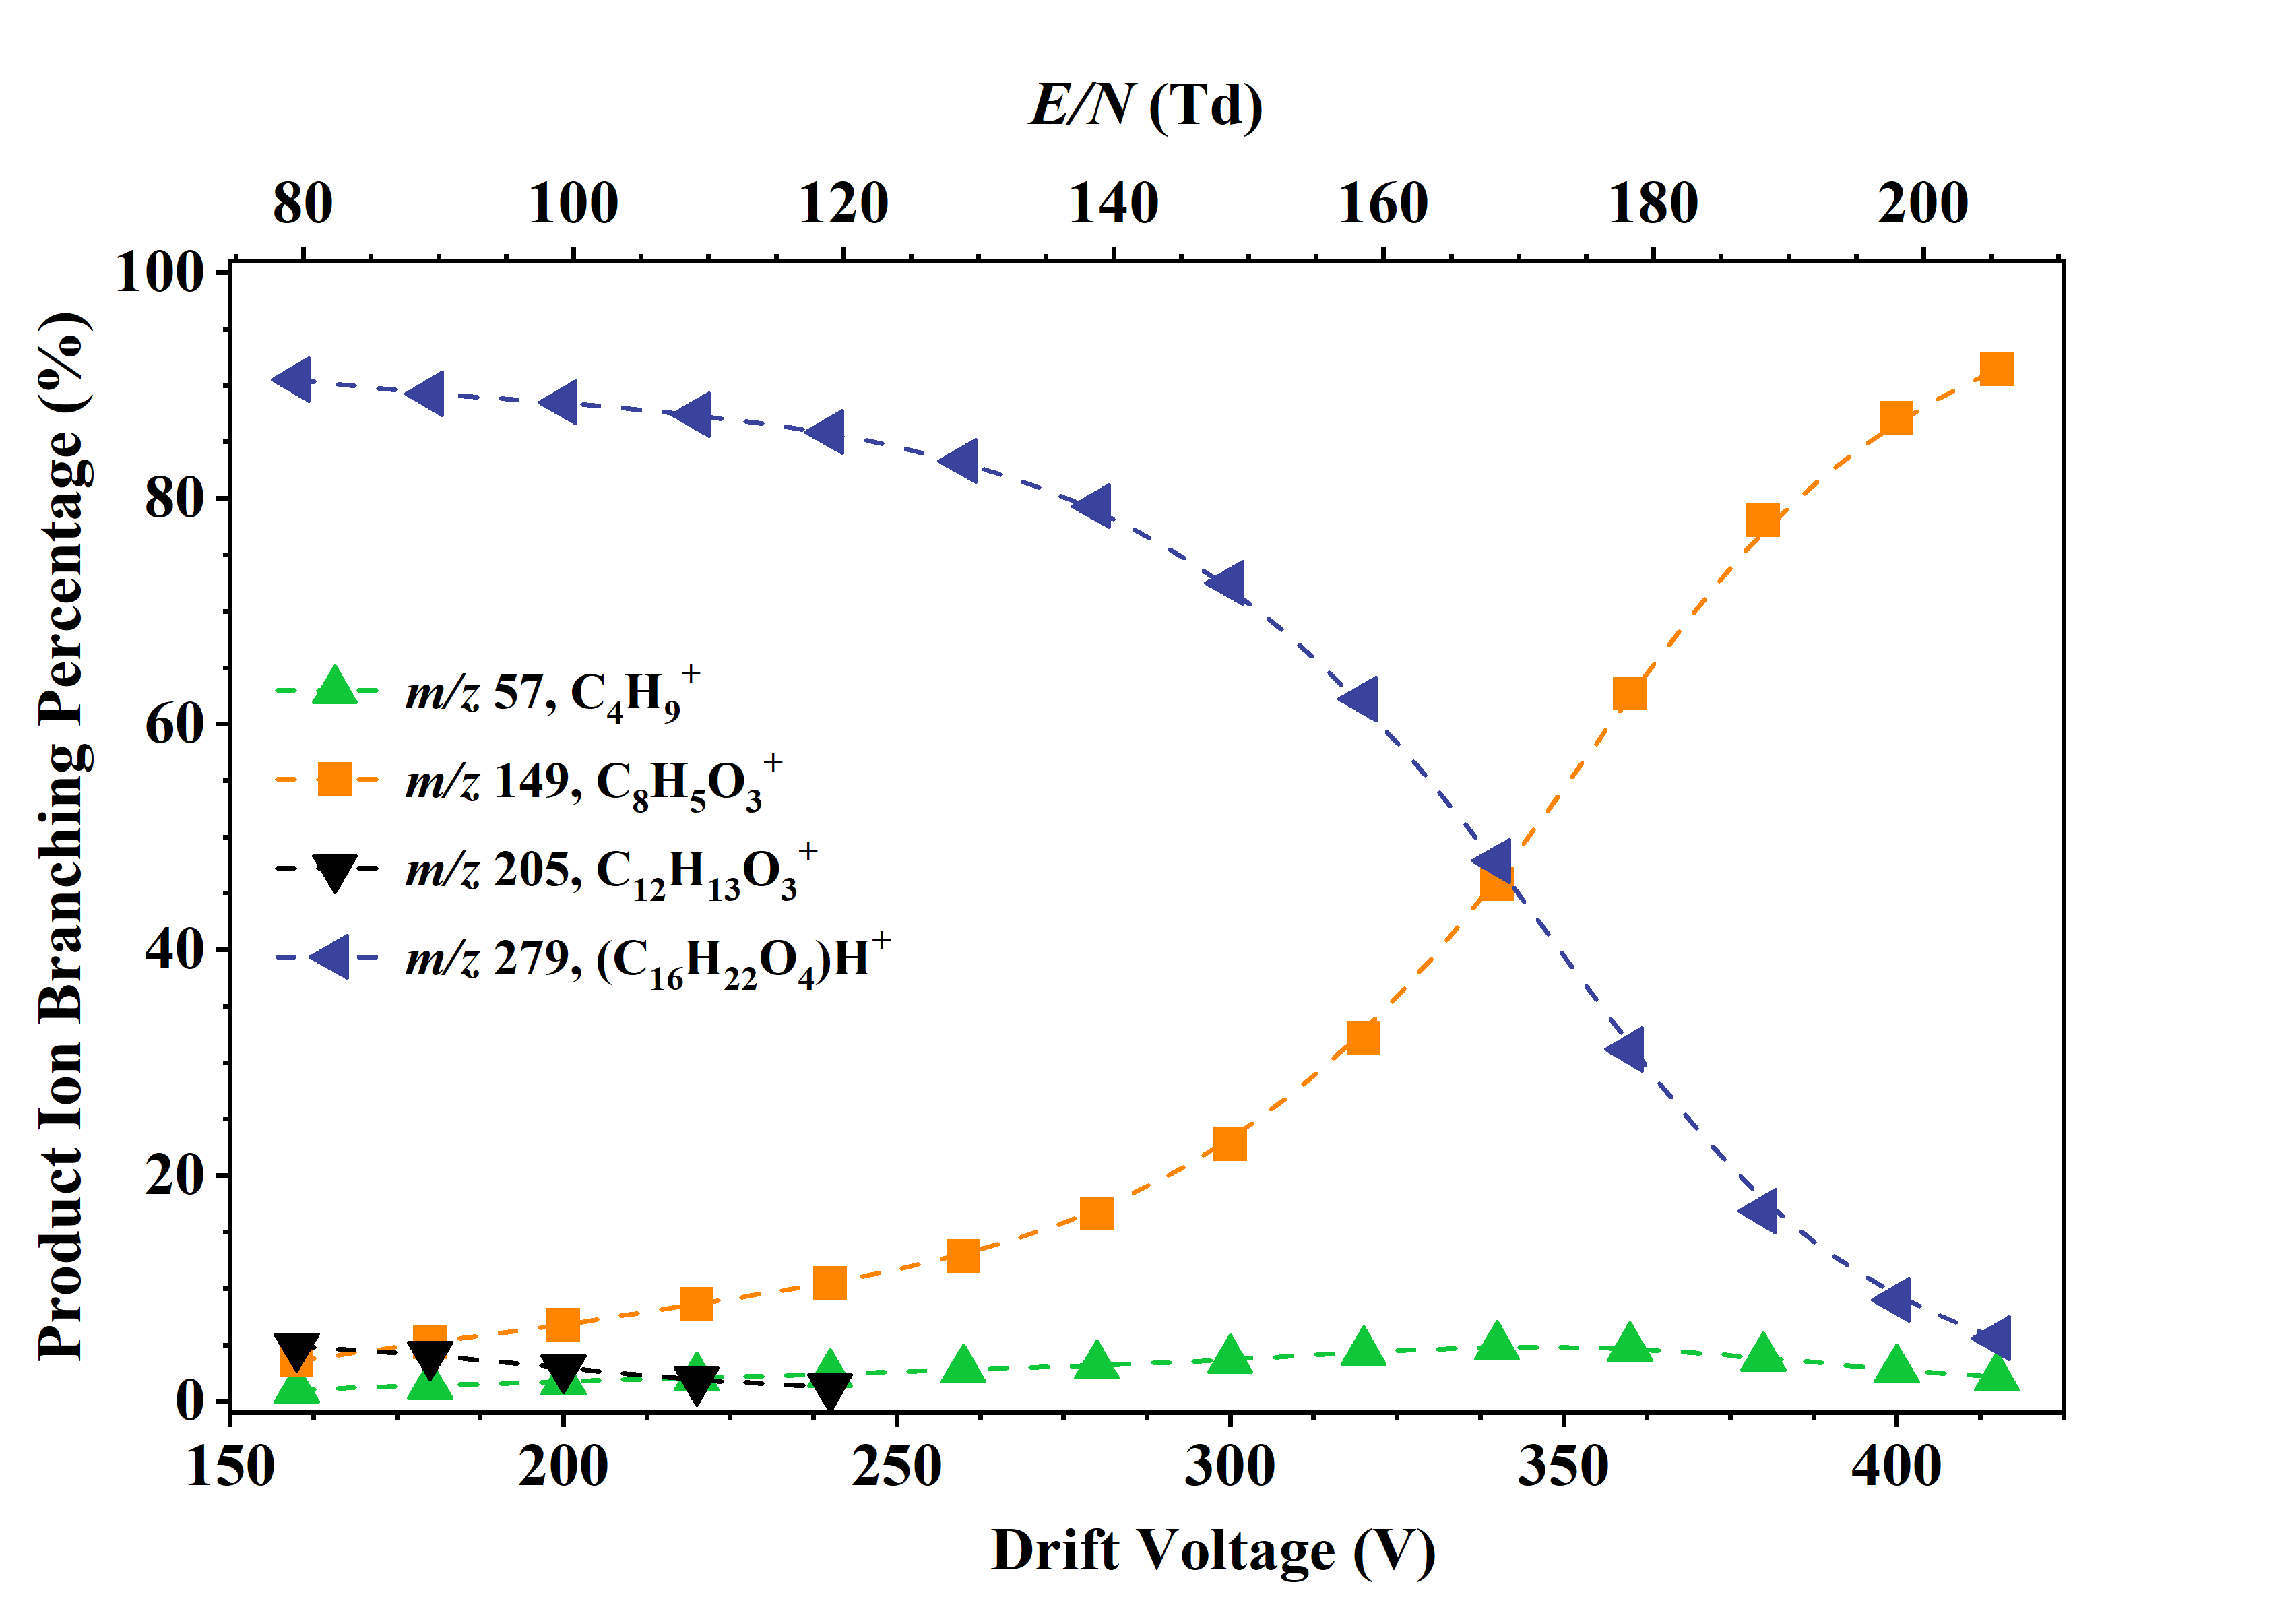
\includegraphics[height=0.4\textheight]{pics/DiBP-BR.png}
\caption{Percentage product ion distribution resulting from the reaction of DiBP with H$_3$O$^+$ as a function of the drift voltage and the reduced electric field in the range from 80 to 205 Td.}
\label{fig:PH_DiBP_fs}
\end{figure}





\subsection{Benzyl butyl phthalate
and dibenzyl phthalate}

BBP and DBeP have a benzyl ester group in common and this seems to be crucial in the proton transfer and fragmentation processes as they show very similar product ion distributions (\autoref{fig:PH_BBP_DBeP_fs}). 
%(\autoref{fig:PH_BBP_fs} for BBP and \autoref{fig:PH_DBeP_fs} for DBeP).
These plots suggest that the protonation sites in the benzyl branch are more basic than in the butyl branch  of BBP.
%
The ion at \textit{m/z} 91, assigned to benzyl radical (C$_7$H$_7^+$), is the dominant ion throughout the whole \textit{E/N} range and this agrees with the mzCloud database \cite{mzcloudBBP}.
%
However, mzCloud also reports protonated phthalic anhydride (i.e. \textit{m/z} 149) and the loss of benzyl alcohol from the protonated parent (i.e. C$_{12}$H$_{13}$O$_3^+$ at \textit{m/z} 205) at the lower collisional energies, but these were not observed in the present PTR-MS measurements. 
%
Furthermore, protonated phthalic anhydride has been reported a major ion for BBP in the literature. For instance, \citeauthor{earls2003gas} monitored protonated phthalic anhydride  in GC-MS to quantify the migration of BBP from PVC toys and childcare products \cite{earls2003gas}.
%
Two other product ions were observed in PTR-MS for both BBP and DBeP with a lower branching percentage than C$_7$H$_7^+$ are
C$_6$H$_7^+$ at \textit{m/z} 79, which is tentatively assigned to protonated benzene, 
and C$_7$H$_7$O$^+$, tentatively assigned to protonated benzaldehyde.

\begin{figure}[htbp]%[htbp]
\centering
\sidesubfloat[]{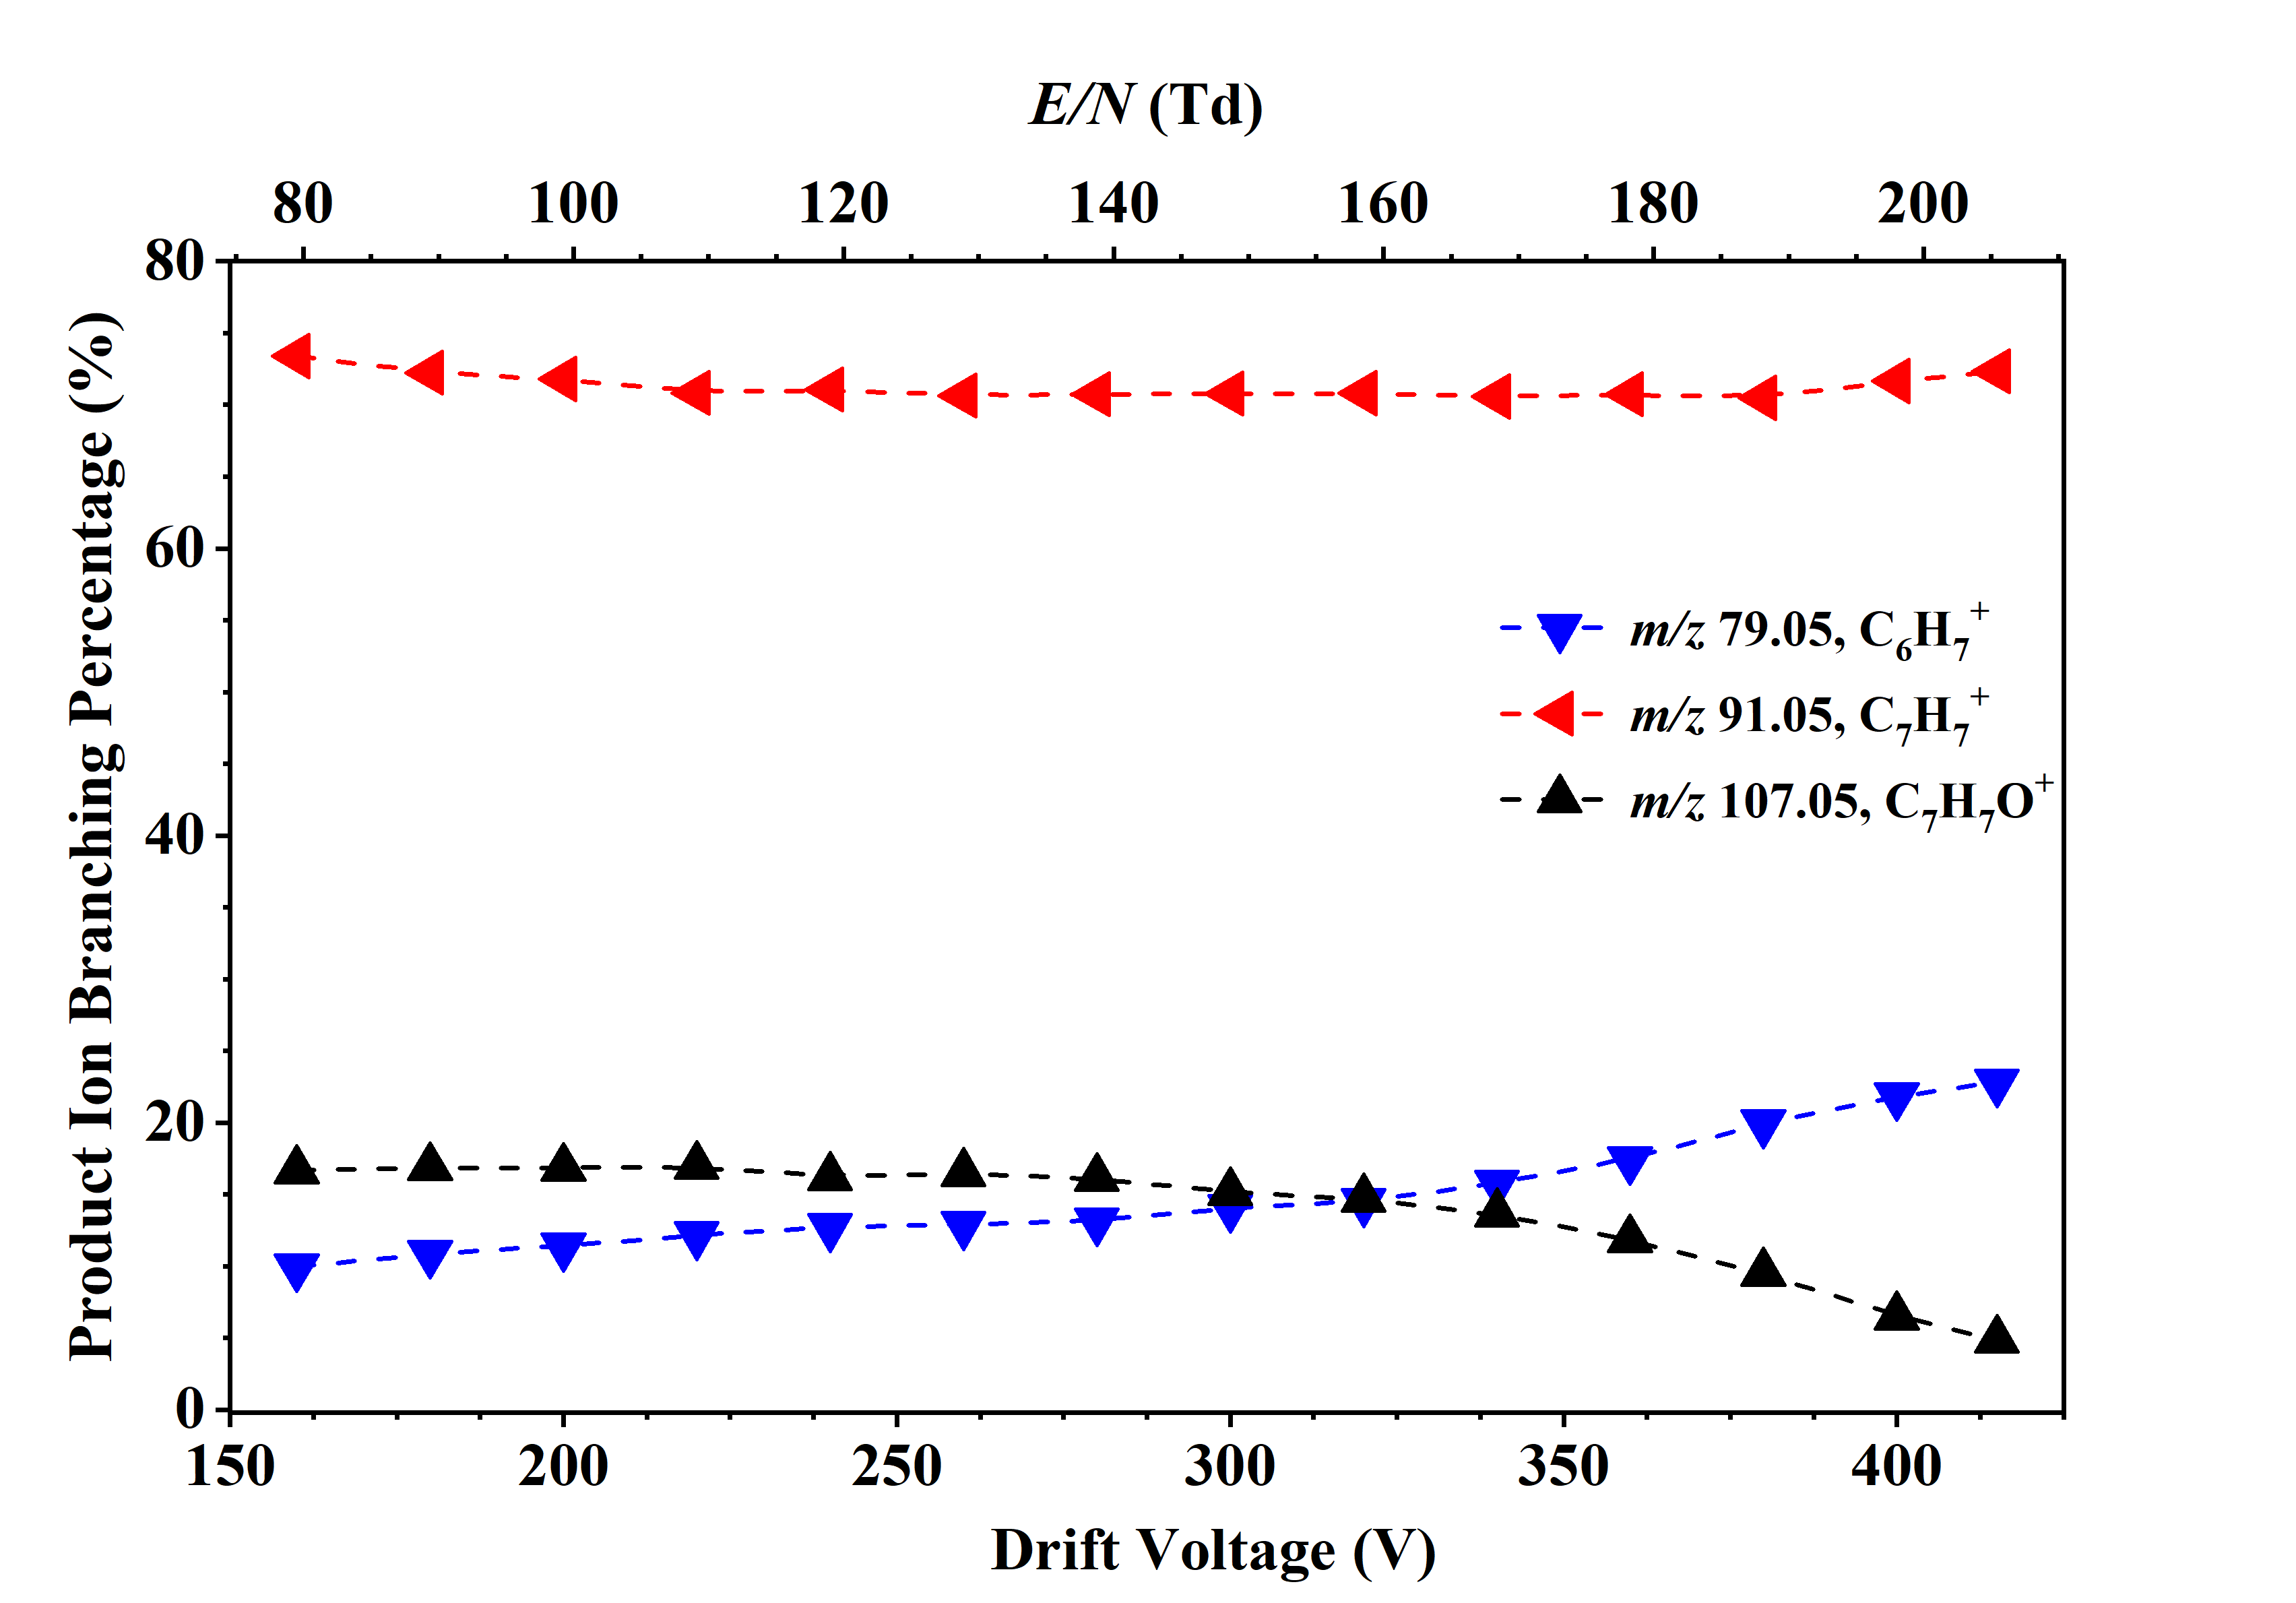
\includegraphics[height=0.4\textheight]{pics/BBP-BR.png}}\\
\sidesubfloat[]{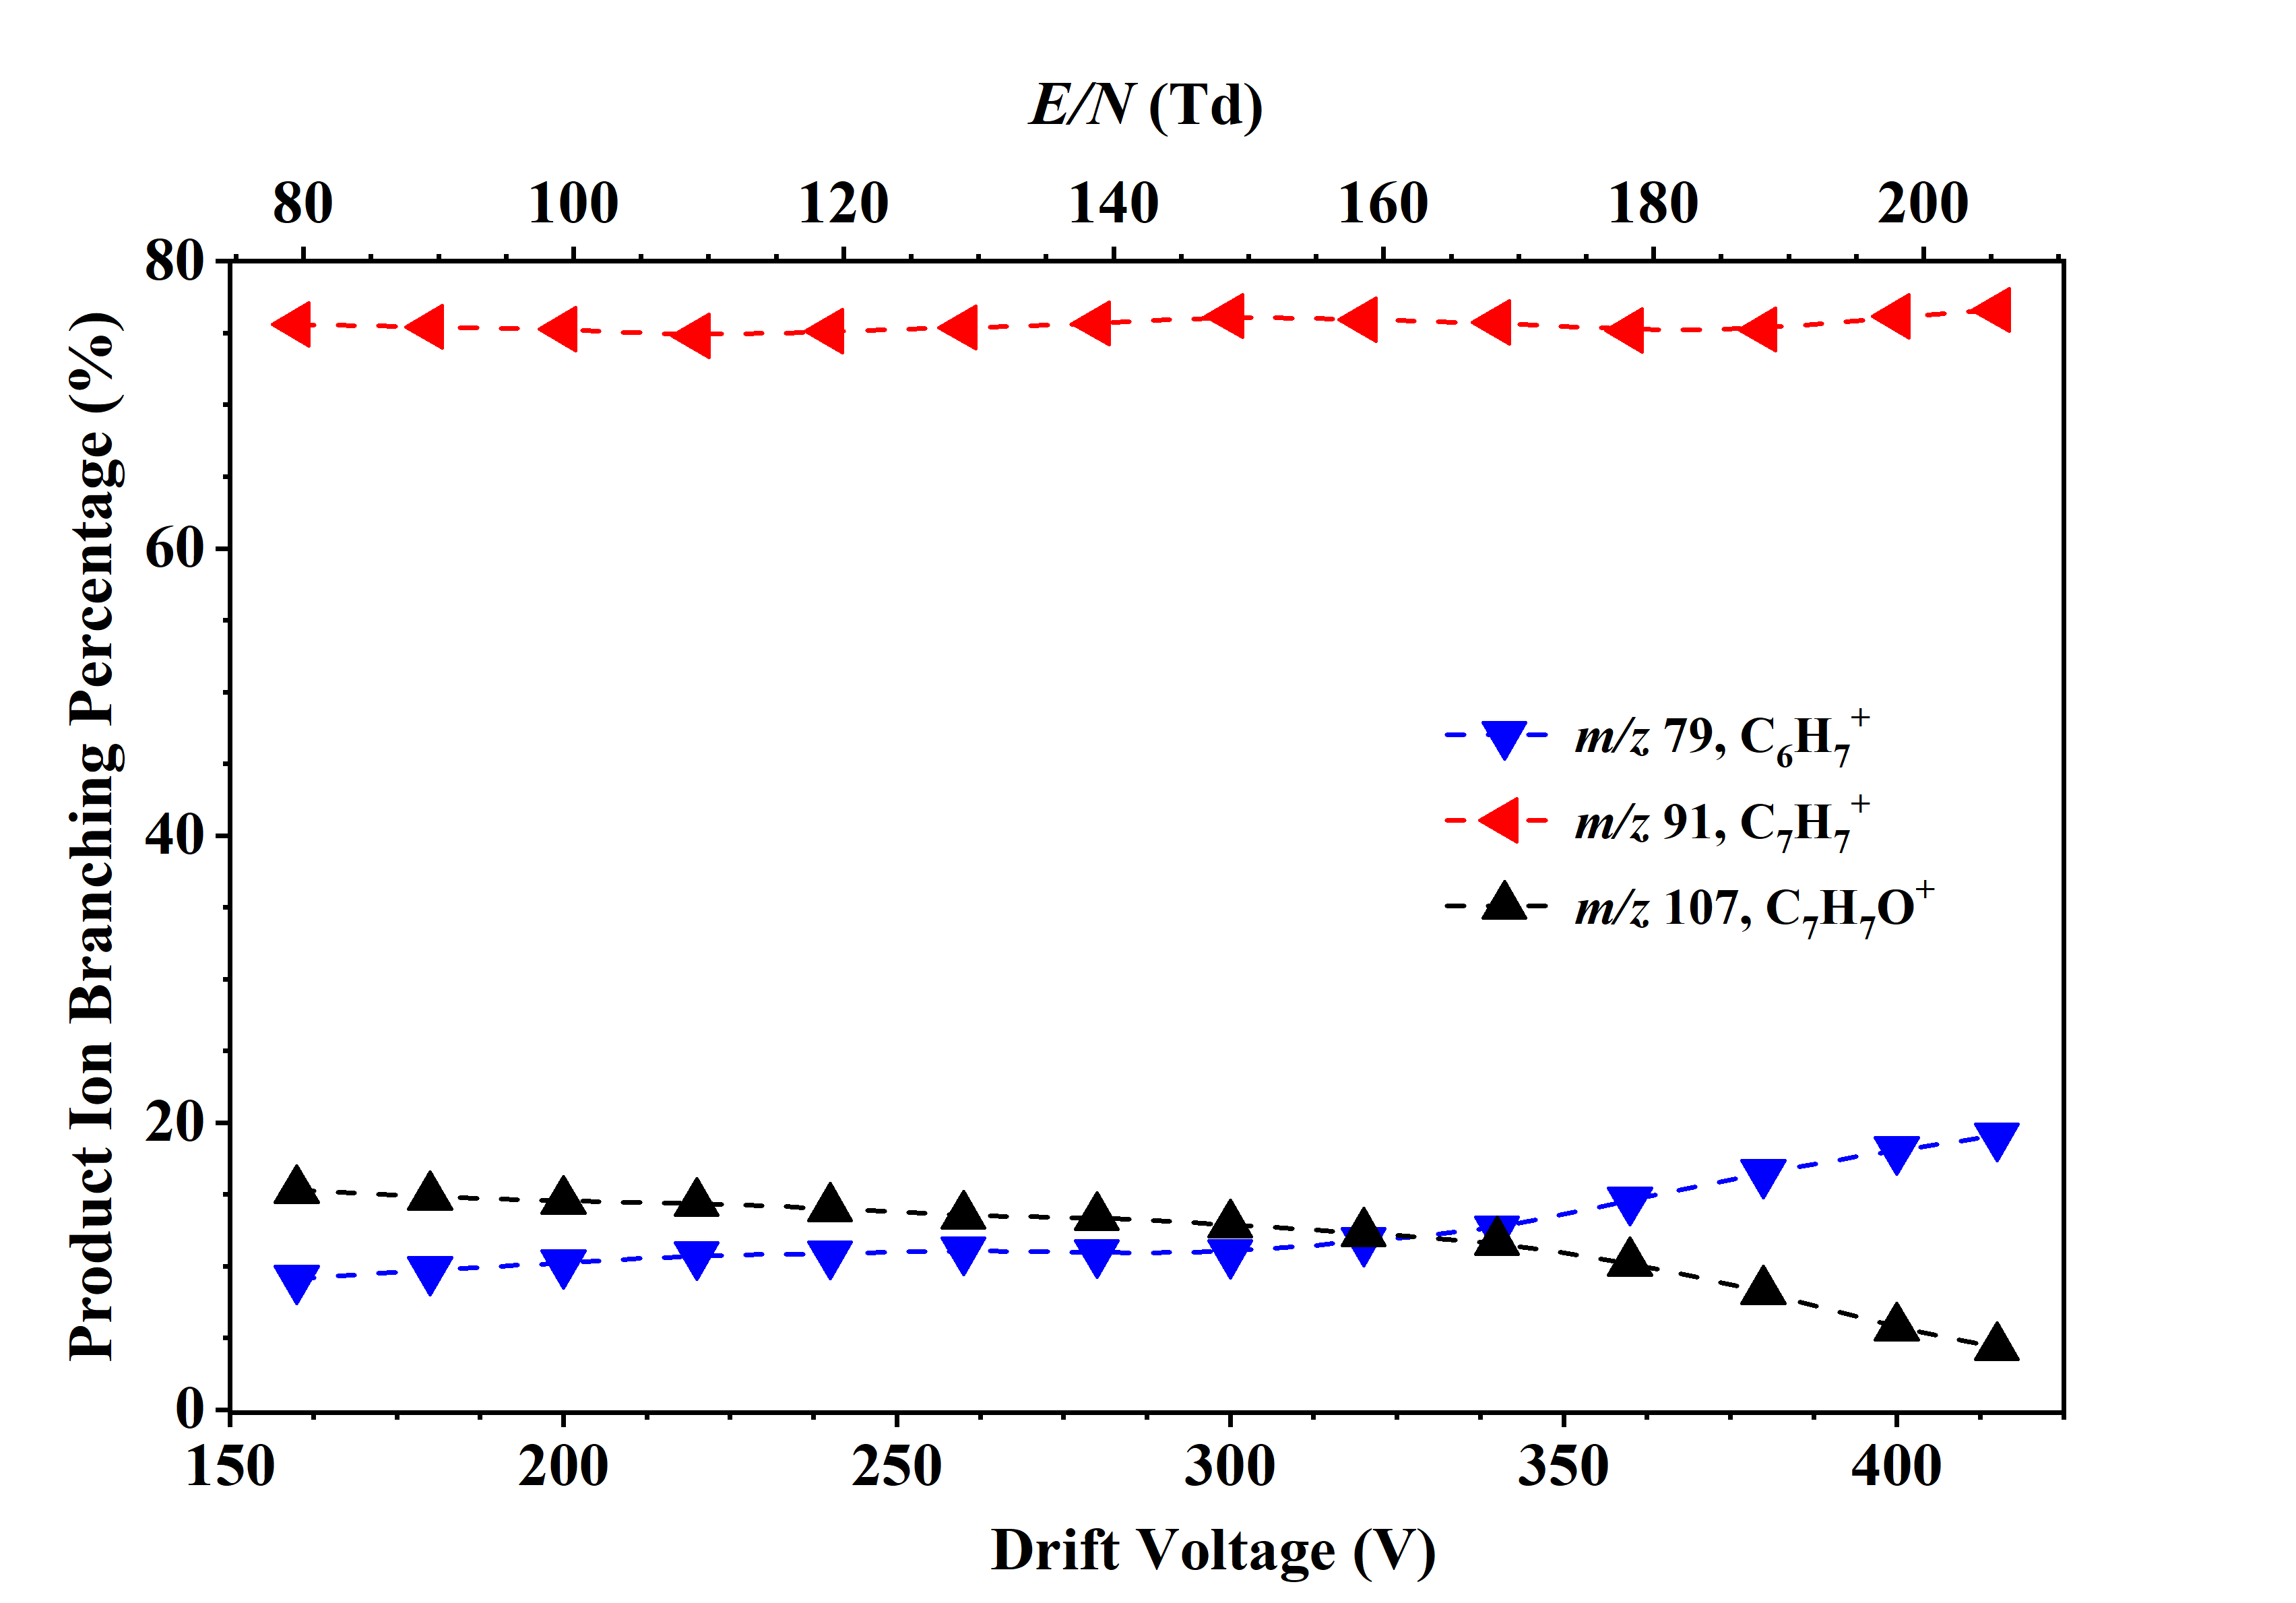
\includegraphics[height=0.4\textheight]{pics/DBeP-BR.png}}
\caption{Percentage product ion distribution resulting from the reaction of (a) BBP and (b) DBeP with H$_3$O$^+$ as a function of the drift voltage and the reduced electric field in the range from 80 to 205 Td.}
\label{fig:PH_BBP_DBeP_fs}
\end{figure}

%\begin{figure}[htb]%[htbp]
%\centering
%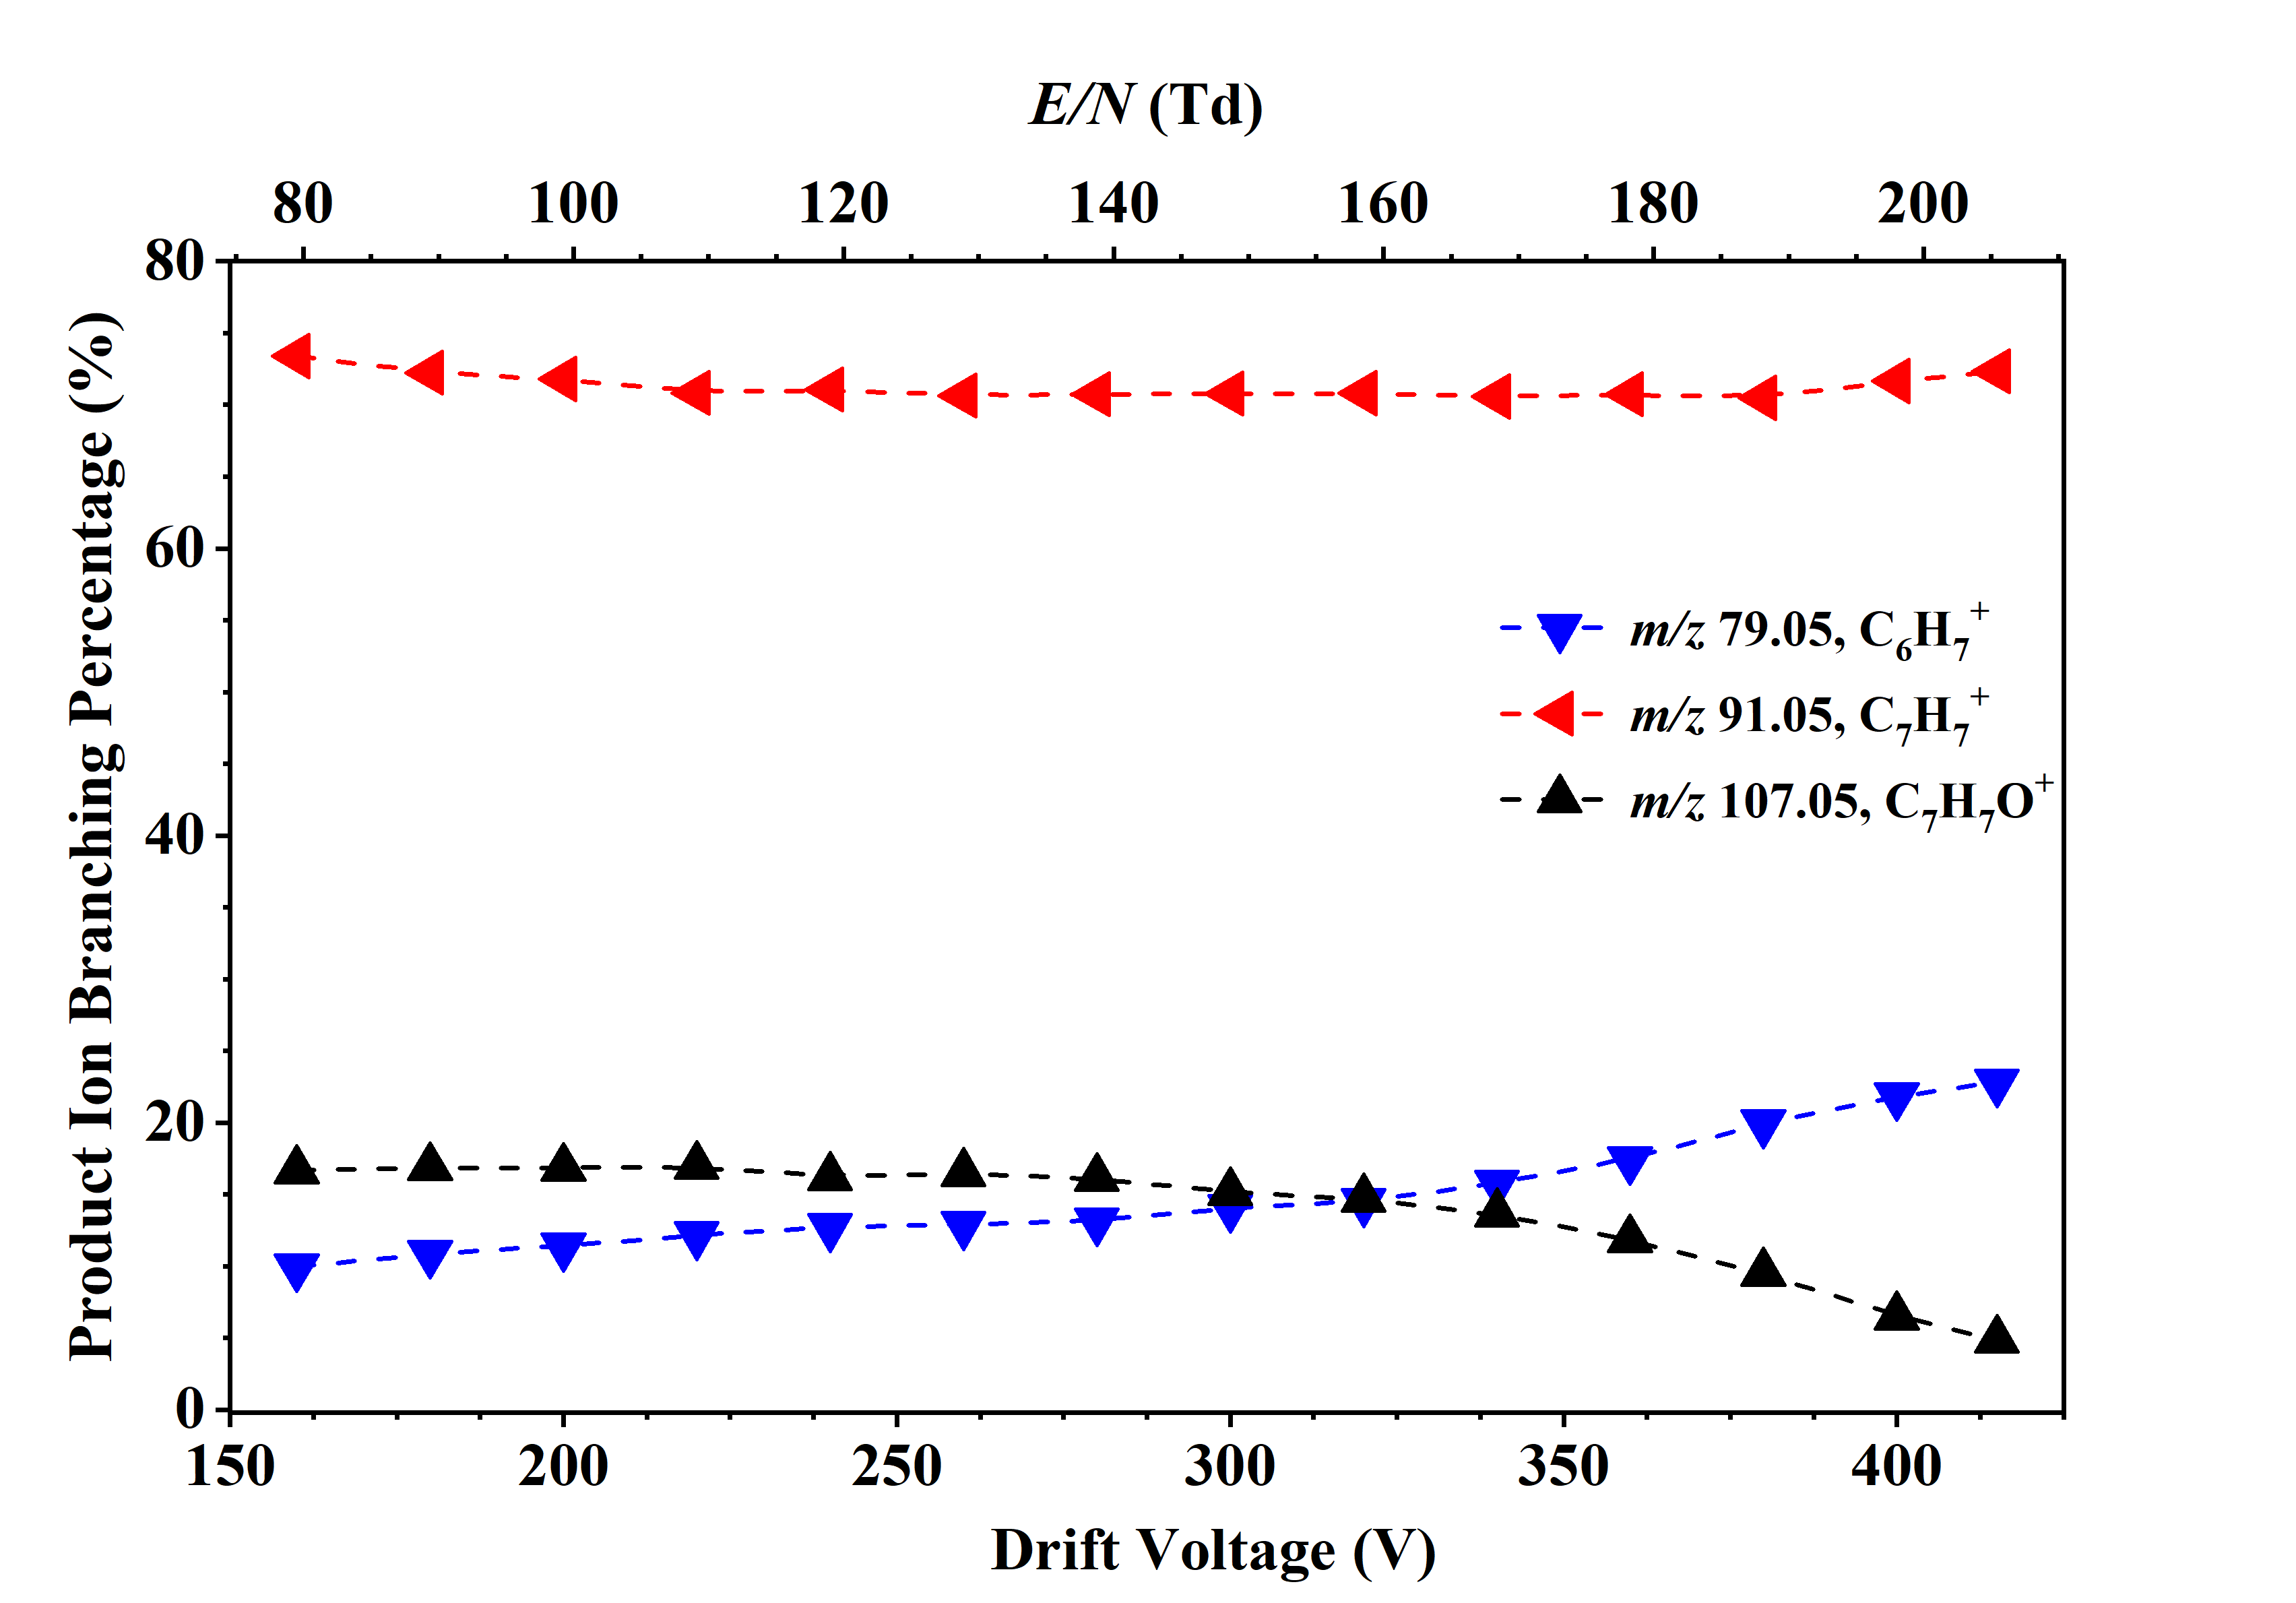
\includegraphics[height=0.4\textheight]{pics/BBP-BR.png}
%\caption{Percentage product ion distribution resulting from the reaction of BBP with H$_3$O$^+$ as a function of the drift voltage and the reduced electric field in the range from 80 to 205 Td.}
%\label{fig:PH_BBP_fs}
%\end{figure}

%\begin{figure}[htb]%[htbp]
%\centering
%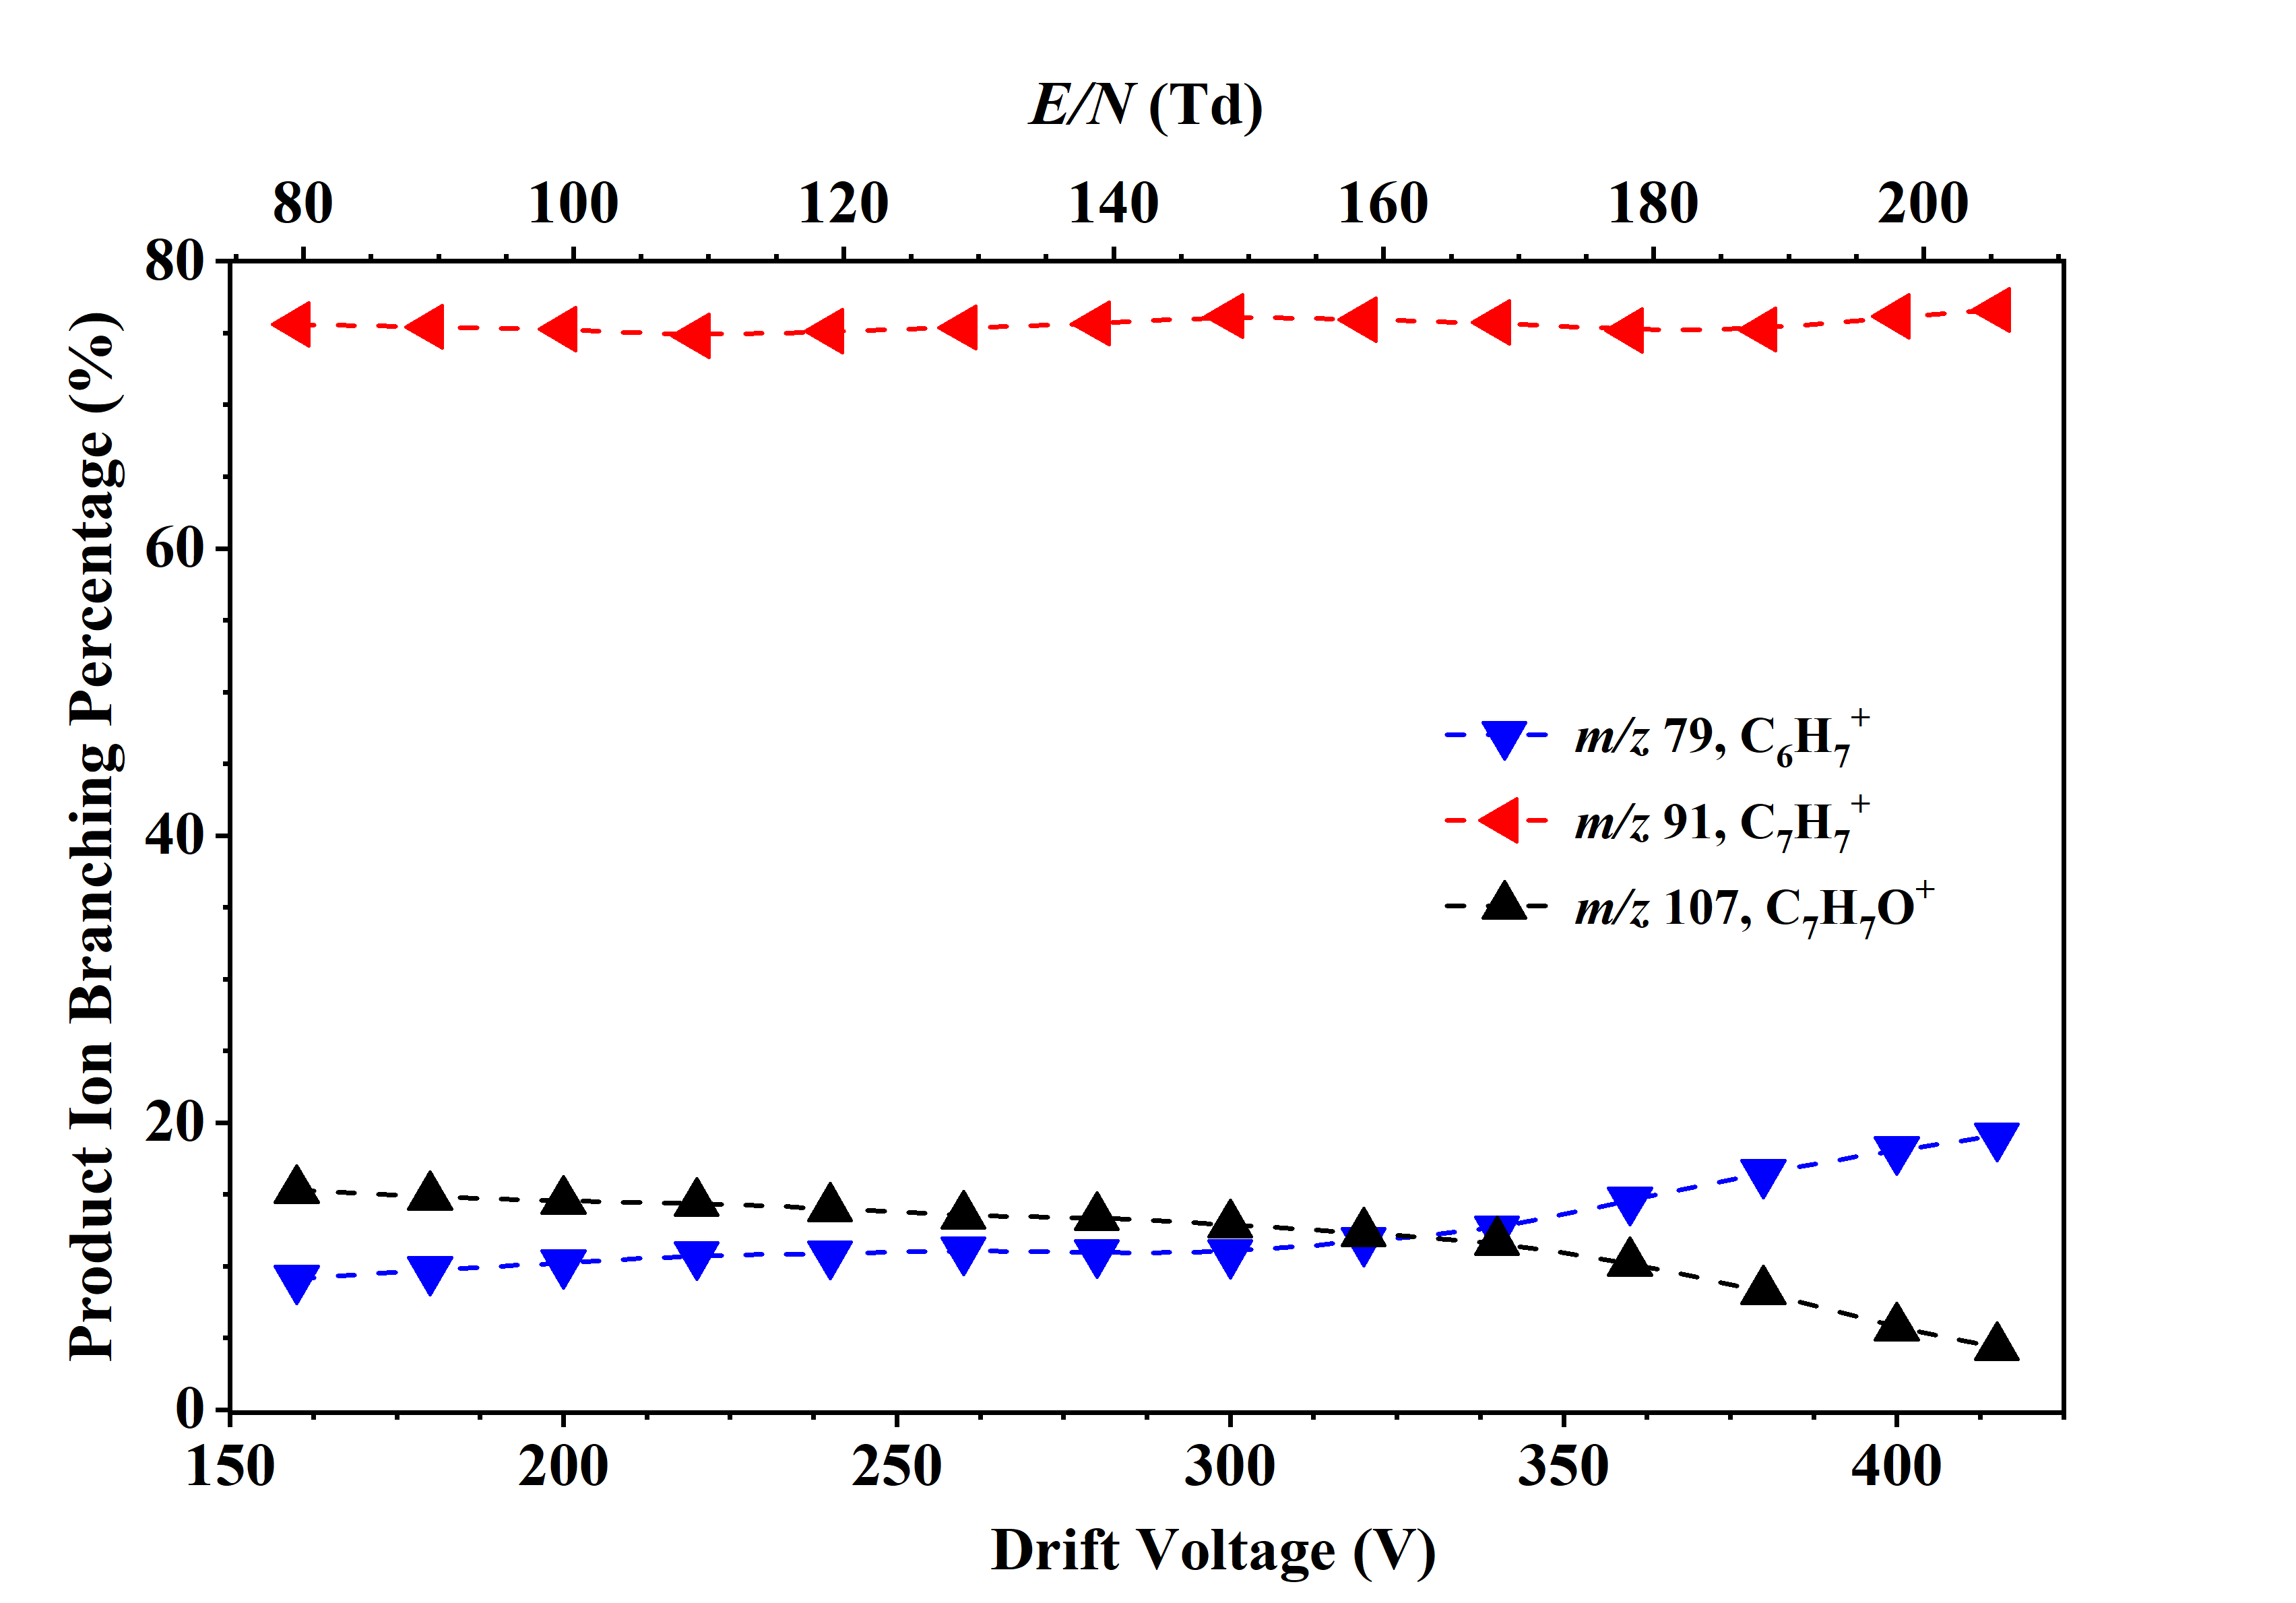
\includegraphics[height=0.4\textheight]{pics/DBeP-BR.png}
%\caption{Percentage product ion distribution resulting from the reaction of DBeP with H$_3$O$^+$ as a function of the drift voltage and the reduced electric field in the range from 80 to 205 Td.}
%\label{fig:PH_DBeP_fs}
%\end{figure}


\subsection{Diethylhexyl phthalate}

DEHP is the most widely used plasticiser. The total world consumption in 2012 was estimated to be of 3 billion tonnes \cite{doi:10.1002/14356007.a20_181.pub2}.
It is anticipated to be a human carcinogen by the \citeauthor{us201614th} \cite{us201614th}.



\autoref{fig:PH_DEHP_fs} shows that the reaction of DEHP with H$_3$O$^+$ yield similar PID results to those of MEHP (\autoref{fig:PH_MEHP_fs}), but the main difference is that here protonated phthalic anhydride is not the dominant ion for DEHP for any \textit{E/N} value. 
%
Instead, there are many ions that become dominant throughout the studied \textit{E/N} range.
%
Furthermore, the only two product ions observed with DEHP that were not found with MEHP are  C$_{15}$H$_{23}$O$_2^+$ at \textit{m/z} 235 and C$_7$H$_{7}$O$_2^+$ at \textit{m/z} 123, tentatively assigned to loss of 2-ethylhexyl formate from the protonated parent ion  and protonated benzoic acid, respectively.

Similarly to MEHP, the ion at \textit{m/z} 279, which would correspond to the loss of C$_8$H$_{16}$ from protonated DEHP, and the protonated parent molecule (C$_{24}$H$_{38}$O$_{4}$)H$^+$ at \textit{m/z} 391
were not observed, although these are reported at low collisional energies in the mzCloud database for ESI-HCD-MS$^2$ analysis of DEHP \cite{mzcloudDEHP}.
%
In said mzCloud results, protonated phthalic anhydride is reported and it is the dominant ion at low collisional energies.
%
Likewise, the hydrocarbon ions at \textit{m/z} 57, \textit{m/z} 71 and \textit{m/z} 113 are also reported in this database but not the ones at \textit{m/z} 39, \textit{m/z} 41 and \textit{m/z} 43 because the cut-off occurs at \textit{m/z} 50.
%
Furthermore, C$_8$H$_7$O$_4^+$ at \textit{m/z} 167, which has the same structure as protonated phthalic acid,  was not observed in PTR-MS but was reported in mzCloud.






\begin{figure}[htb]%[htbp]
\centering
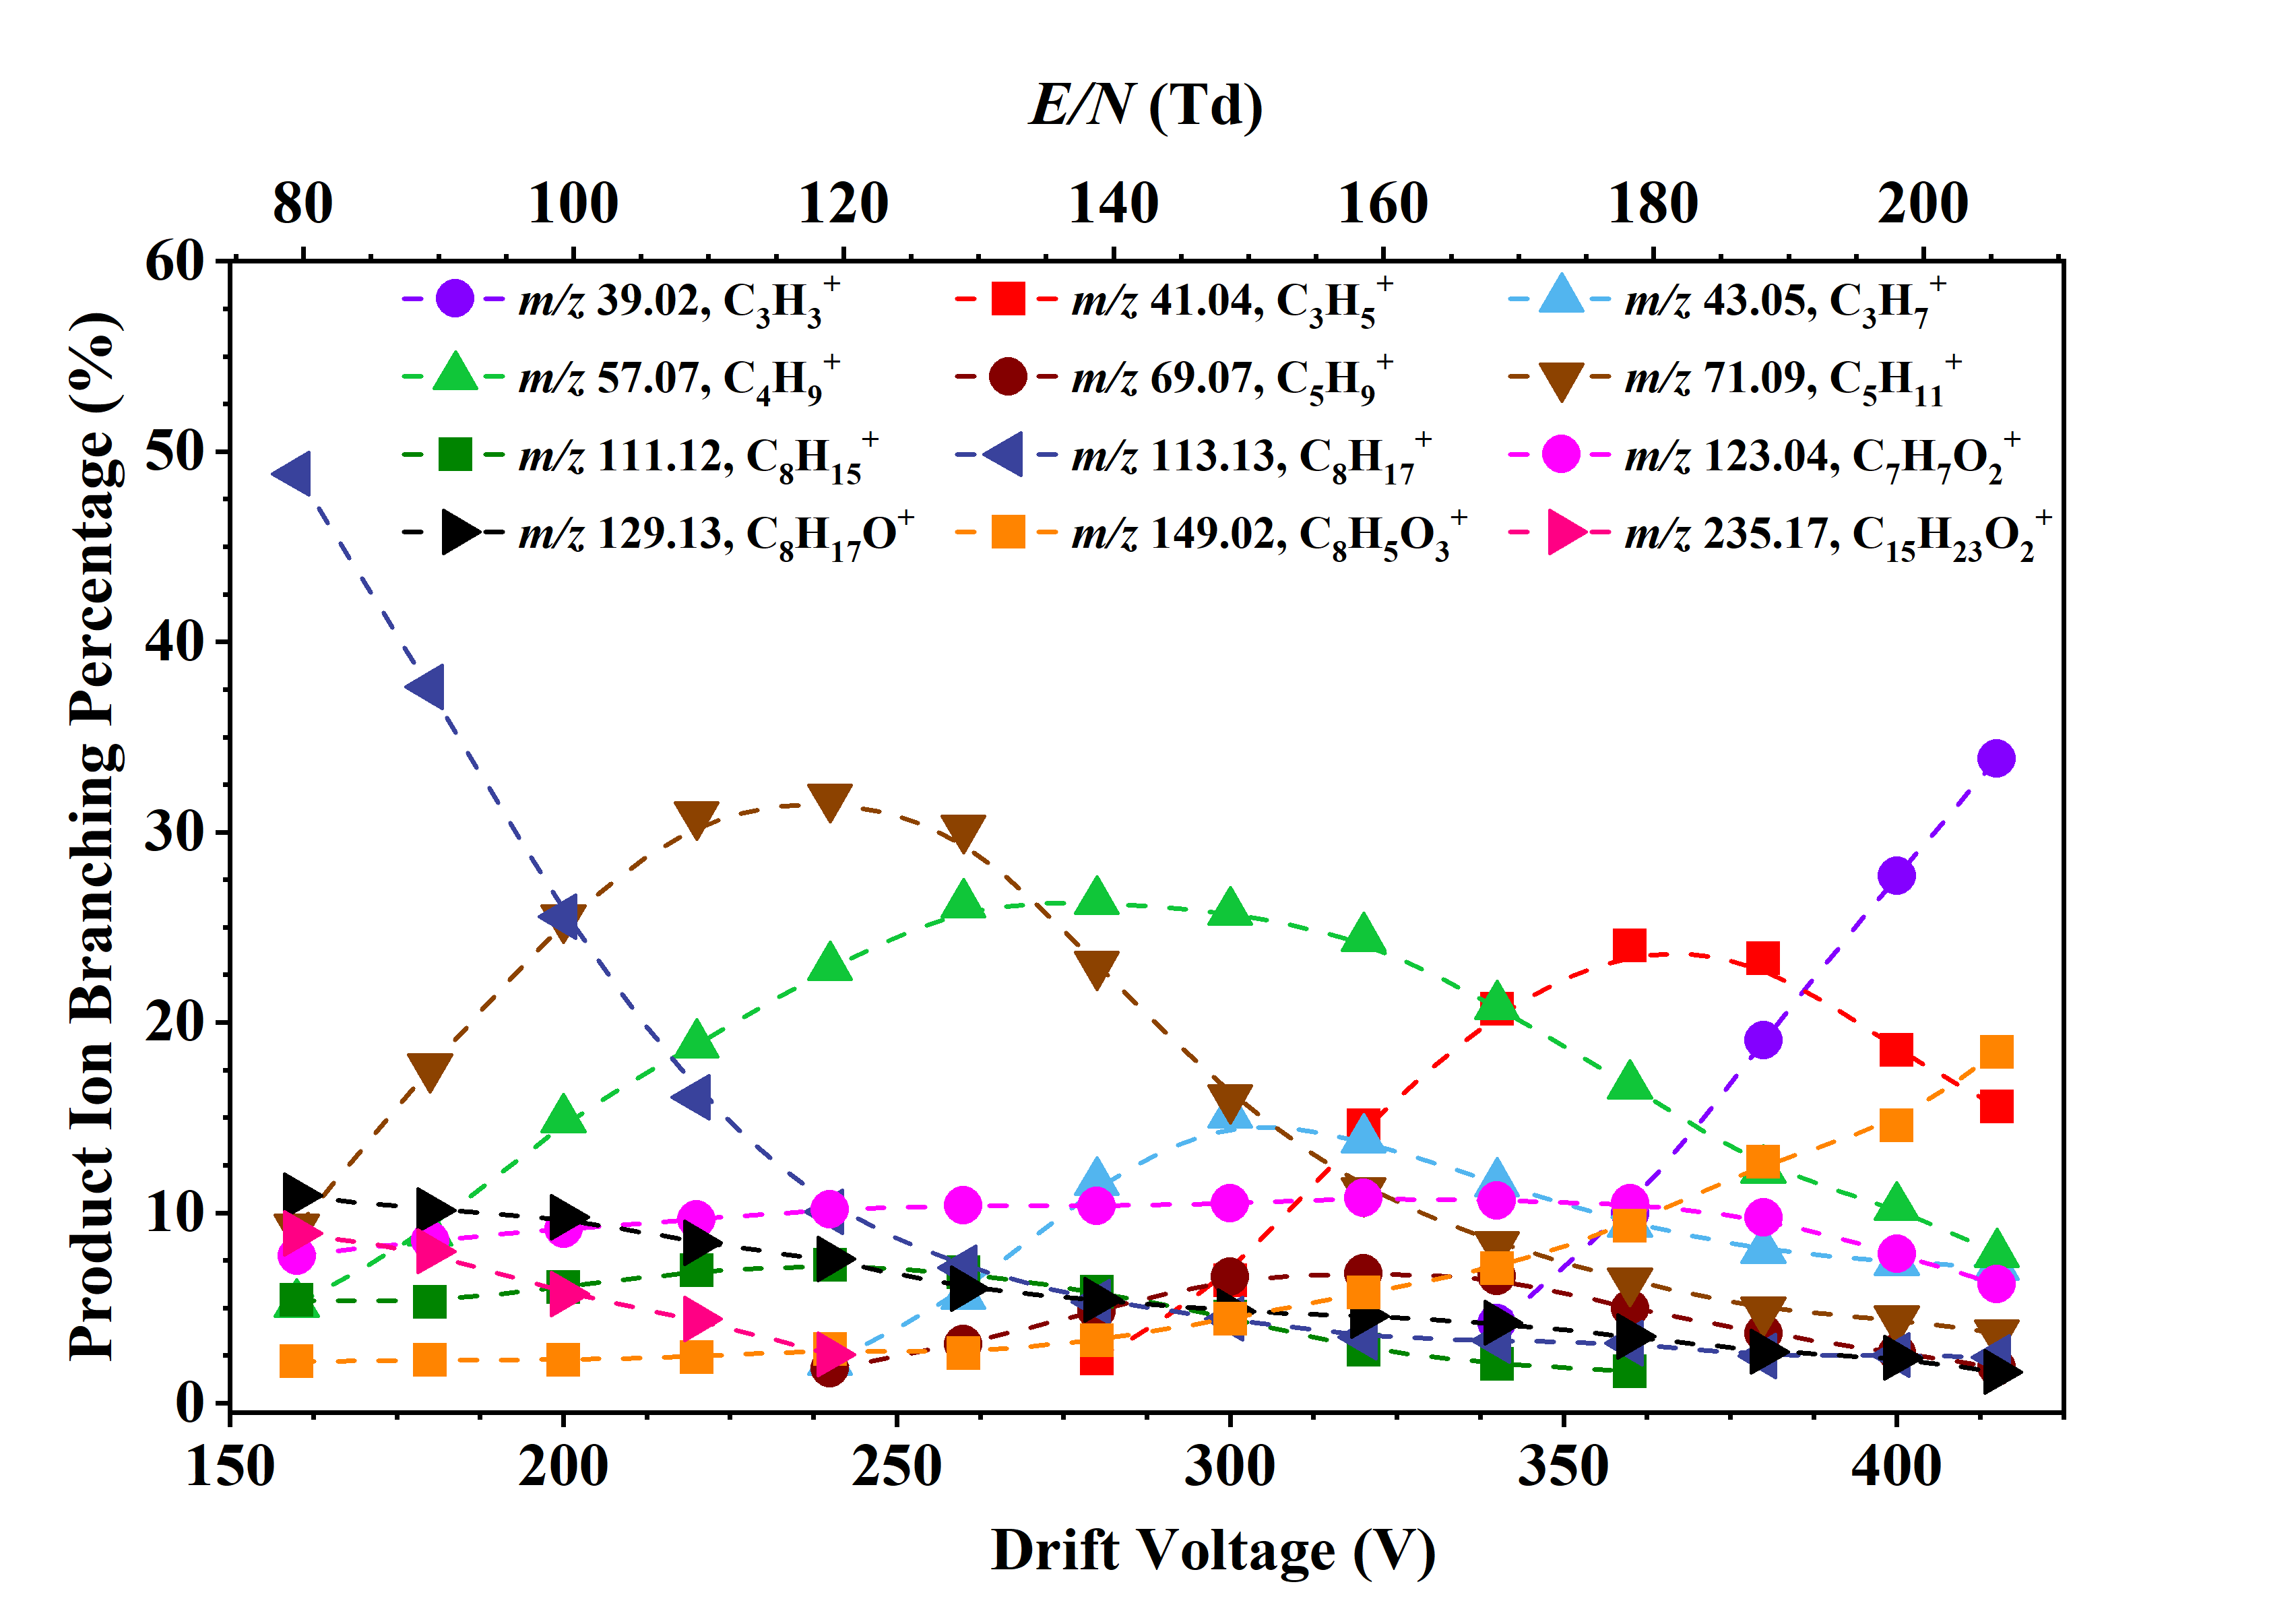
\includegraphics[height=0.4\textheight]{pics/DEHP-BR.png}
\caption{Percentage product ion distribution  resulting from the reaction of DEHP with H$_3$O$^+$ as a function of the drift voltage and the reduced electric field in the range from 80 to 205 Td.}
\label{fig:PH_DEHP_fs}
\end{figure}







\subsection{Separation of isomers: DBP vs DiBP vs MEHP }
DBP, DiBP and MEHP are isomers and thus their protonated parent ion is found at the same \textit{m/z} ((C$_{16}$H$_{22}$O$_4$)H$^+$, \textit{m/z} 279).
%
However, it was found that the reaction of these phthalates with H$_3$O$^+$ yield different product ion distributions at different reduced electric fields that allows to differentiate between them without needing any initial pre-separation.
%
The difference between MEHP and the butyl-containing isomers (i.e. DBP and DiBP)  is the presence of the protonated parent ion at low \textit{E/N} for DBP and DiBP, which is not found for MEHP.
    %
Moreover, to distinguish between DBP and DiBP it is necessary to compare other minor ions.
%
The main differences between these two isomers is the higher signal of C$_{12}$H$_{13}$O$_3^+$ (\textit{m/z} 205) from DBP at low \textit{E/N} (i.e. around 20\%) and C$_{7}$H$_{7}$O$_2^+$ (\textit{m/z} 123) at high E/N, while in the case of DiBP the presence of the former is very little (only ca. 5\%) and the latter is less than 3\% (for this reason it is not included in plots and tables). 















\section{Conclusions}
The study described in the present chapter shows the feasibility of the detection of phthalates in proton transfer reaction mass spectrometry using headspace analysis. 
%
The product ion distributions as a function of the drift voltage and reduced electric field were provided for ten phthalate esters and phthalic acid, including the most relevant phthalates, which are those banned and/or controlled in the EU, USA and China: DBP, BBP and DEHP.
%
Also different product ion distributions were found for  DBP, DiBP and MEHP, which allows to distinguish between these three phthalate ester isomers.
%
The range of collisional energy provided by a PTR-MS instrument has proved to be suitable to see interesting fragmentation pathways from phthalates.
%
Many of the fragmentation channels were only observed at \textit{E/N} higher than a certain value, which indicates that they are a consequence of field-activated collision-induced dissociation.
%
This can be either a pathway that is not thermodynamically allowed or a pathway that, whilst thermodynamically feasible, it is kinetically rather thermodynamically driven.


A characteristic ion found in PTR-MS for many phthalates is protonated phthalic anhydride (\textit{m/z} 149, C$_8$H$_5$O$_2^+$), which is not a surprise as this ion has been widely reported as a phthalate indicator with different mass spectrometric techniques. 
For instance, \citeauthor{mclafferty1989registry} analysed  ca. 140000  EI mass spectra and found that 150 of the 700 spectra where the peak at \textit{m/z} 149  was present corresponded to a phthalate,  so it is a fairly good indicator of the presence of a compound from this family \cite{mclafferty1993interpretation,mclafferty1989registry}. 
%
However, phthalates not always fragment to this ion in PTR-MS and, when \textit{m/z} 149 is observed, its abundance depends on  the reduced electric field. For the alkyl diester phthalates the abundance of protonated phthalic anhydride  increases with the alkyl chain length and with the reduced electric field.
%
Furthermore, looking at the three more strictly regulated phthalates, protonated phthalic anhydride is only the dominant ion for reduced electric field values higher than approx. 130 Td for DBP, while for DEHP it  only reaches  20\% of the total ion signal and for BBP it is not a product ion found in PTR-MS.
%
Therefore, %underestimation can occur and 
caution must be taken before discarding the presence of phthalate esters when \textit{m/z} 149 is not a product ion.





Moreover,  all the studied alkyl diester phthalates lose  the corresponding alcohol (i.e. methanol for DMP, ethanol for DEP, propanol for DPP and butanol for DBP), whose abundance   decreases with  the alkyl chain length. 
%
For instance, for DMP the loss of methanol (\textit{m/z} 163) is the dominant ion throughout all the \textit{E/N} range, while for DBP the loss of butanol (\textit{m/z} 205) is only ca. 20\% at 80 Td and it steadily decreases with the reduced electric field. 
%
Protonated benzoate esters are also product ions observed with phthalates after losing a formate group (e.g. propyl benzoate for DPP, butyl benzoate for DBP and 2-ethylhexyl benzoate for DEHP).








